% =============================================================================
%  Do epiciclo ao integrador simplético: a série de Fourier da órbita
%  kepleriana e os modelos de Copérnico e Ptolomeu
%  Artigo no formato da ABNT NBR 6022 (abnTeX2, opção article).
%  Compilar no Overleaf: Menu > Compiler = pdfLaTeX; o arquivo principal é este.
%  Sequência local: pdflatex main && bibtex main && pdflatex main && pdflatex main
% =============================================================================
\documentclass[
  article,
  12pt,
  a4paper,
  english,          % idioma adicional (abstract)
  brazilian         % idioma principal (último da lista)
]{abntex2}

% ---------------------------------------------------------------- pacotes
\usepackage{lmodern}
\usepackage[T1]{fontenc}
\usepackage[utf8]{inputenc}
\usepackage{indentfirst}
% \usepackage{microtype}   % desligado: deixa cada compilação ~15% mais lenta
\usepackage{amsmath,amssymb,amsthm,mathtools}
\usepackage{icomma}                 % vírgula decimal correta no modo matemático
\usepackage{bm}
\usepackage{graphicx}
\usepackage{xcolor}
\usepackage{booktabs,multirow,array,tabularx}
\usepackage{caption,subcaption}
\usepackage[portuguese,portuguesekw,ruled,vlined,linesnumbered]{algorithm2e}
\usepackage{listings}
\usepackage{tikz}
\usetikzlibrary{arrows.meta,positioning,calc,shapes.geometric,fit,backgrounds}
\usepackage[alf,abnt-emphasize=bf]{abntex2cite}  % citações autor-data (ABNT NBR 10520)

\graphicspath{{figuras/}}

% ---------------------------------------------------------------- comandos do texto
% =============================================================================
%  Comandos, ambientes e estilos usados no texto
% =============================================================================
\usepackage[most]{tcolorbox}

% ---- notação
\newcommand{\vetor}[1]{\bm{#1}}
\newcommand{\vr}{\vetor{r}}
\newcommand{\vv}{\vetor{v}}
\newcommand{\va}{\vetor{a}}
\newcommand{\vh}{\vetor{h}}
\newcommand{\ve}{\vetor{e}}
\newcommand{\dd}{\mathrm{d}}
\newcommand{\ii}{\mathrm{i}}
\newcommand{\UA}{\,\mathrm{UA}}
\newcommand{\dia}{\,\mathrm{dia}}
\newcommand{\km}{\,\mathrm{km}}
\newcommand{\sgn}{\operatorname{sgn}}
\newcommand{\codigo}[1]{\texttt{\small #1}}
\newcommand{\arquivo}[1]{\texttt{\small #1}}

% ---- teoremas (numeração por capítulo)
\theoremstyle{plain}
\newtheorem{proposicao}{Proposição}[section]
\theoremstyle{definition}
\newtheorem{definicao}{Definição}[section]
\newtheorem{exemplo}{Exemplo}[section]
\theoremstyle{remark}
\newtheorem*{observacao}{Observação}

% ---- caixas didáticas
% "Para começar": leitura de entrada, sem cálculo (ensino médio)
\newtcolorbox{paracomecar}[1][]{enhanced,breakable,colback=blue!3,colframe=blue!45!black,
  boxrule=0.5pt,arc=1mm,left=2mm,right=2mm,top=1mm,bottom=1mm,
  fonttitle=\bfseries\small,title={Para começar#1}}
% "Para aprofundar": detalhe técnico que pode ser pulado na primeira leitura
\newtcolorbox{paraaprofundar}[1][]{enhanced,breakable,colback=orange!4,colframe=orange!60!black,
  boxrule=0.5pt,arc=1mm,left=2mm,right=2mm,top=1mm,bottom=1mm,
  fonttitle=\bfseries\small,title={Para aprofundar#1}}
% "Lição de projeto": um erro real que o projeto cometeu e corrigiu
\newtcolorbox{licao}[1][]{enhanced,breakable,colback=red!3,colframe=red!50!black,
  boxrule=0.5pt,arc=1mm,left=2mm,right=2mm,top=1mm,bottom=1mm,
  fonttitle=\bfseries\small,title={Lição de projeto#1}}
% "No programa": onde a ideia aparece na tela
\newtcolorbox{noprograma}[1][]{enhanced,breakable,colback=green!3,colframe=green!40!black,
  boxrule=0.5pt,arc=1mm,left=2mm,right=2mm,top=1mm,bottom=1mm,
  fonttitle=\bfseries\small,title={No programa#1}}

% ---- código-fonte
\definecolor{fundocodigo}{RGB}{248,248,250}
\definecolor{comentario}{RGB}{90,110,90}
\definecolor{palavra}{RGB}{20,60,150}
\definecolor{textocod}{RGB}{150,40,40}
\lstdefinelanguage{TypeScript}{
  keywords={const,let,var,function,return,if,else,for,while,break,continue,new,
    export,import,from,type,interface,readonly,as,of,in,throw,true,false,null,undefined},
  morekeywords=[2]{number,string,boolean,void,Float64Array,Math},
  sensitive=true,
  morecomment=[l]{//},
  morecomment=[s]{/*}{*/},
  morestring=[b]',
  morestring=[b]",
  morestring=[b]`
}
\lstset{
  basicstyle=\ttfamily\scriptsize,
  backgroundcolor=\color{fundocodigo},
  keywordstyle=\color{palavra}\bfseries,
  keywordstyle=[2]\color{palavra},
  commentstyle=\color{comentario}\itshape,
  stringstyle=\color{textocod},
  numbers=left, numberstyle=\tiny\color{gray}, numbersep=6pt,
  frame=single, rulecolor=\color{gray!40}, framexleftmargin=4pt,
  breaklines=true, breakatwhitespace=false, columns=fullflexible, keepspaces=true,
  showstringspaces=false, tabsize=2, captionpos=t,
  literate={á}{{\'a}}1 {é}{{\'e}}1 {í}{{\'i}}1 {ó}{{\'o}}1 {ú}{{\'u}}1
           {Á}{{\'A}}1 {É}{{\'E}}1 {Í}{{\'I}}1 {Ó}{{\'O}}1 {Ú}{{\'U}}1
           {ã}{{\~a}}1 {õ}{{\~o}}1 {Ã}{{\~A}}1 {Õ}{{\~O}}1
           {â}{{\^a}}1 {ê}{{\^e}}1 {ô}{{\^o}}1 {Â}{{\^A}}1 {Ê}{{\^E}}1 {Ô}{{\^O}}1
           {ç}{{\c c}}1 {Ç}{{\c C}}1 {à}{{\`a}}1 {ü}{{\"u}}1
           {—}{{---}}1 {−}{{-}}1 {·}{{$\cdot$}}1 {×}{{$\times$}}1 {≤}{{$\le$}}1 {≥}{{$\ge$}}1
           {π}{{$\pi$}}1 {μ}{{$\mu$}}1 {√}{{$\surd$}}1 {°}{{$^\circ$}}1 {≈}{{$\approx$}}1
}
\renewcommand{\lstlistingname}{Código}
\renewcommand{\lstlistlistingname}{Lista de códigos}

% ---- algoritmos
\SetAlgoCaptionSeparator{ --}
\SetKwComment{Com}{$\triangleright$\ }{}
\SetAlFnt{\small}
% palavras-chave em português (independe da versão do algorithm2e)
\SetKwInput{KwIn}{Entrada}
\SetKwInput{KwOut}{Saída}
\SetKwFor{For}{para}{faça}{fim}
\SetKwFor{ForEach}{para cada}{faça}{fim}
\SetKwFor{While}{enquanto}{faça}{fim}
\SetKwIF{If}{ElseIf}{Else}{se}{então}{senão se}{senão}{fim}
\SetKw{KwTo}{até}
\SetKw{Return}{retorne}


% ---------------------------------------------------------------- dados do trabalho
\title{Do epiciclo ao integrador simplético: a série de Fourier da órbita kepleriana e os modelos de Copérnico e Ptolomeu}
\author{Filipi Ramos \and Thiago Vinícius\thanks{Curso de Ciência da Computação, Instituto Brasiliense de Direito Público (IDP), sob a supervisão do Prof.\ Alexandre.}}
\date{}

% ---------------------------------------------------------------- PDF
\makeatletter
\hypersetup{
  pdftitle={Do epiciclo ao integrador simplético: a série de Fourier da órbita kepleriana e os modelos de Copérnico e Ptolomeu},
  pdfauthor={Filipi Ramos; Thiago Vinícius},
  pdfkeywords={epiciclos, séries de Fourier, problema de N corpos, integrador simplético, ensino de física},
  colorlinks=true,
  linkcolor=blue!50!black,
  citecolor=blue!50!black,
  urlcolor=blue!50!black,
  bookmarksdepth=4
}
\makeatother

\setlength{\parindent}{1.3cm}
\setlength{\parskip}{0.2cm}
\OnehalfSpacing

\begin{document}
\selectlanguage{brazilian}
\frenchspacing

% ------------------------------------------------ título, resumo e abstract
\begin{center}
  {\large\bfseries Do epiciclo ao integrador simplético: a série de Fourier da órbita kepleriana e os modelos de Copérnico e Ptolomeu\par}
  \vspace{1em}
  Filipi Ramos e Thiago Vinícius\footnote{Curso de Ciência da Computação, Instituto Brasiliense de Direito Público (IDP), sob a supervisão do Prof.\ Alexandre.}
\end{center}
\setlength{\absparsep}{12pt}
\begin{resumo}
Por que os epiciclos de Ptolomeu e Copérnico descreviam tão bem o céu? Desenvolvemos um simulador do Sistema Solar que integra a gravitação mútua do Sol e dos oito planetas a partir de condições iniciais do JPL Horizons, com o integrador simplético de Yoshida de quarta ordem e passo fixo de meio dia. Contra a efeméride DE440s, numa varredura de $-100$ a $+100$ anos, o desvio fica abaixo de 0,5\,\% da distância ao Sol; no pior caso, Mercúrio, chega a 0,46\,\% e a 13 minutos de arco na direção vista da Terra. A energia oscila sem crescer. Sobre essas órbitas, calculamos a série de Fourier complexa parametrizada no tempo, com forma fechada em funções de Bessel. Até primeira ordem na excentricidade, ela tem a estrutura da construção do \emph{Commentariolus}: um deslocamento fixo de $\tfrac{3}{2}ae$, um deferente de raio $a$ e um epiciclo de raio $\tfrac{1}{2}ae$ com o dobro da frequência. Os raios de Copérnico para Marte, Júpiter e Saturno concordam com esses valores em até 8\,\%, e a razão de três para um entre os seus epiciclos, herdada da substituição do equante, coincide com a da série. O equante de Ptolomeu, usado como controle, tem o mesmo conteúdo de primeira ordem: com parâmetros modernos e o deferente de Copérnico igual a $|c_1|$, ele, o modelo de Copérnico e a série erram a posição de Marte em cerca de 0,007\,UA, os três em ordem $e^2$. A série explica por que os dois modelos funcionam.

\textbf{Palavras-chave}: epiciclos. séries de Fourier. problema de $N$ corpos. integrador simplético. Copérnico.
\end{resumo}

\begin{resumo}[Abstract]
\begin{otherlanguage*}{english}
This report describes a Solar System simulator for teaching physics, mathematics and computing, in which the instructor chooses how deep the explanation goes, from high school to graduate level. The project started from an undergraduate thesis that compared Copernicus' epicycles with the Fourier series of planetary orbits \cite{farias2016} and had three versions: a Python prototype that rebuilds the Kepler ellipse from a Fourier series; a two-dimensional version, in Python and Pygame, that integrates the mutual gravitation of the Sun and the eight planets from JPL Horizons initial conditions; and a three-dimensional version, in TypeScript and three.js, with thirteen moons, real imaging textures, a Fourier laboratory and a body-creation sandbox. The dynamics use Yoshida's fourth-order symplectic integrator with a fixed half-day step. Against JPL's reference ephemeris, the error stays below 0.5\,\% of the heliocentric distance on the five dates tested, from $-100$ to $+100$ years, and the energy oscillates around its initial value instead of drifting. The text covers the physical background (gravitation, the two-body problem, orbital elements, Kepler's equation), the mathematical background (complex Fourier series, epicycles, sampling, symplectic integrators), the implementation choices and the test-driven development process. On the thesis' question, we show, in agreement with analyses in the literature, that the complex Fourier series of a Keplerian orbit, to first order in the eccentricity, has the structure of Copernicus' construction: a fixed offset of $\tfrac{3}{2}ae$, a deferent of radius $a$ and an epicycle of radius $\tfrac{1}{2}ae$ turning at twice the frequency. The radii in the \emph{Commentariolus} for Mars, Jupiter and Saturn agree with these values to within 10\,\%. We did not compare this result with other models of the same order, such as Ptolemy's with equant, and the classroom uses suggested here have not been tested with students.

\vspace{\onelineskip}
\noindent
\textbf{Keywords}: epicycles. Fourier series. $N$-body problem. symplectic integrator. physics education.
\end{otherlanguage*}
\end{resumo}


% ------------------------------------------------ elementos textuais
\section{Introdução}\label{cap:introducao}
% orçamento: 700 palavras

Ptolomeu descreveu o movimento dos planetas com círculos montados sobre círculos. Copérnico mudou o centro e manteve os círculos. Kepler trocou os círculos por elipses, e Newton mostrou de onde as elipses vêm.

Este artigo apresenta um programa que simula o Sistema Solar pela lei da gravitação de Newton, a partir de posições e velocidades do JPL/NASA, e que mostra cada órbita também como uma cadeia de epiciclos. Usamos o programa para responder a uma pergunta antiga com ferramentas modernas: por que os epiciclos funcionavam tão bem, e o que os números de Copérnico têm a ver com a série de Fourier de uma órbita kepleriana.

\subsection{Origem do projeto}

A pergunta vem do trabalho de conclusão de curso de \citeonline{farias2016}, \emph{Copérnico estava certo? Uma análise de epiciclos e séries de Fourier}, defendido na Faculdade UnB Planaltina. O TCC perguntou se as órbitas de Mercúrio, Vênus, Marte, Júpiter e Saturno podem ser escritas como somas de senos e cossenos, e comparou os raios dos epiciclos que Copérnico publicou no \emph{Commentariolus} com os raios obtidos da série de Fourier. Concluiu que dois ou três termos da série já reproduzem bem as órbitas e que os raios de Copérnico têm a ordem de grandeza certa.

Partimos da mesma pergunta com duas diferenças. A órbita vem de uma integração numérica de nove corpos validada contra o JPL, e não de uma elipse ideal. E a série é calculada no tempo, e não no ângulo, o que muda os coeficientes e permite uma comparação direta com o mecanismo de Copérnico (\autoref{sec:param-tempo}).

\subsection{Objetivos}

O objetivo geral é desenvolver um simulador do Sistema Solar fisicamente fundamentado, validado contra dados de referência, e usá-lo para examinar a relação entre a série de Fourier de uma órbita e os modelos de epiciclos. Os objetivos específicos são:

\begin{enumerate}
  \item integrar o problema gravitacional de $N$ corpos com um método que conserve a energia a longo prazo, partindo de condições iniciais do JPL Horizons;
  \item medir o erro das posições calculadas contra a efeméride de referência do JPL;
  \item reconstruir a órbita de cada corpo por série de Fourier complexa e exibir a cadeia de epiciclos correspondente;
  \item comparar, planeta a planeta, os raios do modelo de Copérnico com os coeficientes da série.
\end{enumerate}

\subsection{Contribuições}

\begin{itemize}
  \item um simulador que roda em navegador comum, sem acesso à internet durante o uso, e que publica o próprio erro medido contra o JPL;
  \item uma exposição autocontida da cadeia que vai da lei de Newton à série de Fourier de uma órbita, com a forma fechada dos coeficientes em funções de Bessel conferida numericamente;
  \item a constatação de que a série complexa da órbita kepleriana, até primeira ordem na excentricidade, tem a estrutura do modelo do \emph{Commentariolus} (deslocamento de $\tfrac{3}{2}ae$, deferente e epiciclo de $\tfrac{1}{2}ae$ com frequência dupla), em acordo com análises da literatura \cite{gallavotti2001,sugon2008}, acompanhada de uma comparação numérica com os raios de Copérnico.
\end{itemize}

\subsection{Organização do texto}

A \autoref{cap:historia} resume o contexto histórico, de Ptolomeu a Newton. A \autoref{cap:matematica} desenvolve a série de Fourier de uma órbita kepleriana até a forma fechada dos coeficientes e a aproximação de primeira ordem. A \autoref{sec:metodo} descreve a física do simulador, o integrador e a validação. A \autoref{cap:resultados} reúne os resultados quantitativos, incluindo a comparação com Copérnico. A \autoref{sec:discussao} discute limitações e usos possíveis em sala de aula, e a \autoref{cap:conclusao} conclui. Os apêndices trazem derivações e instruções para reproduzir os resultados.

\section{Contexto histórico: dos epiciclos à gravitação}\label{cap:historia}
% orçamento: 1.100 palavras

O resumo histórico a seguir é breve e segue as fontes usadas por \citeonline{farias2016}. Um tratamento mais extenso está em \cite{kuhn2002,martins2003,damasio2011,linton2004}.

\subsection{O problema dos planetas}

Para quem observa o céu a olho nu, as estrelas giram juntas, como se estivessem presas a uma esfera. Cinco pontos luminosos não seguem esse movimento. Mercúrio, Vênus, Marte, Júpiter e Saturno caminham devagar contra o fundo de estrelas, sempre perto da faixa do zodíaco, e de tempos em tempos param, recuam e voltam a avançar. Esse recuo é o \emph{movimento retrógrado}, e foi o grande desafio da astronomia antiga.

O próprio simulador reproduz o fenômeno. A \autoref{fig:marte-retrogrado} mostra a longitude eclíptica de Marte visto da Terra, calculada pelo programa a partir das condições iniciais de 1º de janeiro de 2026. Entre 10 de janeiro e 1º de abril de 2027 a longitude diminui: Marte anda para trás no céu. No plano de longitude e latitude, o caminho desenha o laço característico.

\begin{figure}[htb]
  \centering
  \caption{Movimento retrógrado de Marte em 2027, calculado pelo simulador}
  \label{fig:marte-retrogrado}
  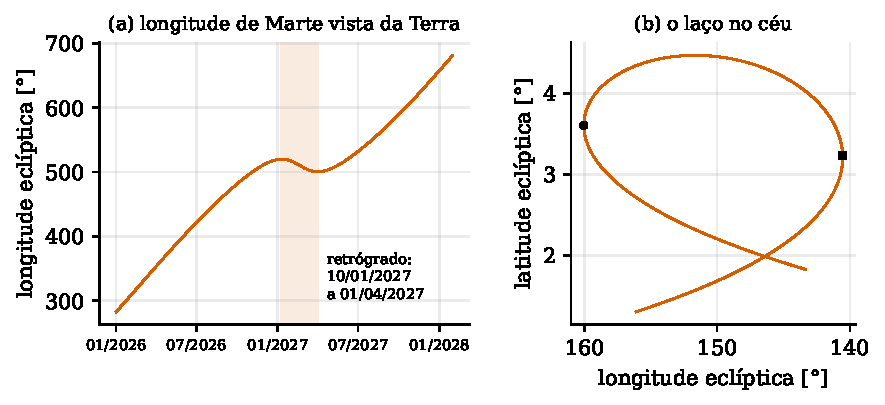
\includegraphics[width=\textwidth]{marte_retrogrado.pdf}
  \legend{(a) Longitude eclíptica geocêntrica de Marte ao longo de dois anos; a faixa sombreada marca o intervalo em que ela decresce. (b) O mesmo intervalo no plano longitude--latitude, com o eixo de longitude invertido como no céu: o círculo e o quadrado marcam o início e o fim da retrogradação. Fonte: elaborada pelos autores com o integrador descrito na \autoref{sec:integradores}.}
\end{figure}

Hoje sabemos que o recuo é efeito de perspectiva: a Terra anda mais depressa que Marte e, quando o ultrapassa, por algumas semanas Marte parece andar para trás.

\subsection{Ptolomeu: deferente, epiciclo, excêntrico e equante}

No \emph{Almagesto}, por volta de 150 d.C., Cláudio Ptolomeu reuniu a astronomia grega em um sistema matemático capaz de prever as posições dos planetas \cite{linton2004}. A Terra fica imóvel e cada planeta se move sobre um círculo pequeno, o \emph{epiciclo}, cujo centro percorre um círculo grande, o \emph{deferente}. A composição dos dois movimentos produz os laços retrógrados.

Dois refinamentos completam o modelo (\autoref{fig:ptolomeu}). O centro do deferente não coincide com a Terra: ele fica deslocado, num \emph{excêntrico}. E o centro do epiciclo não gira com velocidade angular constante em torno do centro do deferente nem em torno da Terra, mas em torno de um terceiro ponto, o \emph{equante}, simétrico à Terra em relação ao centro. O equante fazia o modelo concordar com as observações, mas violava o ideal de movimento circular uniforme, e foi isso que mais incomodou Copérnico \cite{farias2016,damasio2011}.

\begin{figure}[htb]
  \centering
  \caption{Elementos do modelo de Ptolomeu}
  \label{fig:ptolomeu}
  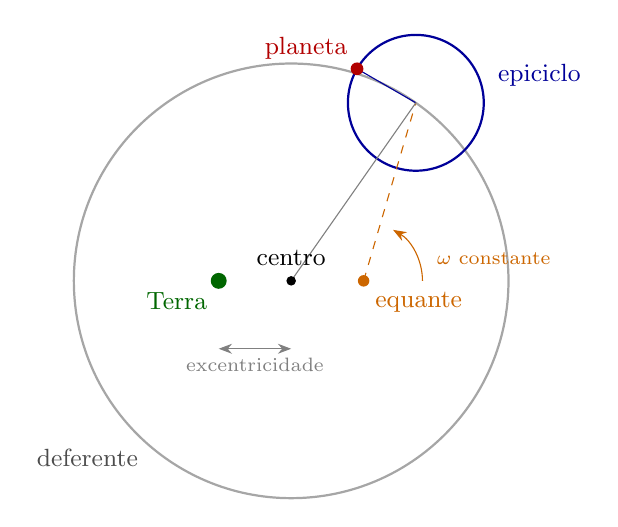
\begin{tikzpicture}[scale=1.15,>=Stealth]
    \def\R{2.4}
    \coordinate (C) at (0,0);
    \coordinate (T) at (-0.8,0);
    \coordinate (Q) at (0.8,0);
    \draw[thick,gray!70] (C) circle (\R);
    \node[gray!60!black,font=\small] at (-2.25,-1.95) {deferente};
    \coordinate (P) at (55:\R);
    \draw[thick,blue!60!black] (P) circle (0.75);
    \node[blue!60!black,font=\small,anchor=west] at ($(P)+(0.8,0.3)$) {epiciclo};
    \coordinate (Pl) at ($(P)+(150:0.75)$);
    \draw[blue!60!black] (P) -- (Pl);
    \fill[red!70!black] (Pl) circle (2pt) node[above left,font=\small] {planeta};
    \draw[dashed,orange!80!black] (Q) -- (P);
    \draw[gray] (C) -- (P);
    \fill (C) circle (1.5pt) node[above=2pt,font=\small] {centro};
    \fill[green!40!black] (T) circle (2.5pt) node[below left=1pt,font=\small] {Terra};
    \fill[orange!80!black] (Q) circle (1.8pt) node[below right=1pt,font=\small] {equante};
    \draw[<->,gray] ($(T)+(0,-0.75)$) -- node[below,font=\scriptsize]{excentricidade} ($(C)+(0,-0.75)$);
    \draw[->,orange!80!black] ($(Q)+(0.65,0)$) arc (0:60:0.65);
    \node[orange!80!black,font=\scriptsize,anchor=west] at ($(Q)+(0.7,0.25)$) {$\omega$ constante};
  \end{tikzpicture}
  \legend{O centro do epiciclo percorre o deferente com velocidade angular constante vista do equante, e não do centro nem da Terra. Fonte: elaborada pelos autores, a partir de \citeonline{linton2004} e \citeonline{farias2016}.}
\end{figure}

\subsection{Copérnico: o mesmo círculo, outro centro}

Nicolau Copérnico (1473--1543) apresentou o heliocentrismo primeiro num manuscrito curto, o \emph{Commentariolus}, que circulou por volta de 1514, e depois no \emph{De revolutionibus orbium coelestium}, publicado em 1543 \cite{martins2003,kuhn2002}. Com o Sol no centro, o movimento retrógrado deixa de exigir um epiciclo próprio para cada planeta: ele aparece naturalmente quando a Terra ultrapassa um planeta externo, ou é ultrapassada por um interno.

Copérnico, porém, não abandonou os círculos. Para reproduzir as variações de velocidade que Ptolomeu explicava com o equante, ele usou epiciclos menores. A substituição do equante por dois epiciclos não é exclusiva de Copérnico: Ibn al-Shatir, em Damasco, no século XIV, já usava o mesmo dispositivo \cite{kennedy1959,swerdlow1973}. No \emph{Commentariolus}, cada planeta tem um deferente e dois epiciclos, e o centro do deferente não é o Sol: é o centro da órbita da Terra, o chamado Sol médio, que fica um pouco deslocado do Sol verdadeiro. Os raios são dados em \emph{partes}, com o raio da órbita da Terra dividido em 25 partes \cite{martins2003,farias2016}. A \autoref{tab:copernico-raios} reproduz esses valores.

\begin{table}[htb]
  \centering
  \caption{Raios do deferente e dos epiciclos no \emph{Commentariolus}}
  \label{tab:copernico-raios}
  \begin{tabular}{lccc}
    \toprule
    Planeta & Deferente $R$ & 1º epiciclo $r_1$ & 2º epiciclo $r_2$ \\
    \midrule
    Mercúrio & $9 + 2/5$ & $1 + 41'$ & $34'$ \\
    Vênus    & $18$ & $3/4$ & $1/4$ \\
    Marte    & $38$ & $5 + 34'$ & $1 + 51'$ \\
    Júpiter  & $130 + 5/12$ & $10 + 6'$ & $3 + 22'$ \\
    Saturno  & $230 + 1/6$ & $19 + 41'$ & $6 + 34'$ \\
    \bottomrule
  \end{tabular}
  \legend{Valores em partes, com o raio da órbita terrestre igual a 25 partes; o símbolo $'$ indica sessenta avos de parte. O deferente de Marte segue a correção de Rosen adotada por \citeonline{farias2016}: os manuscritos trazem 30. Fonte: \citeonline{farias2016}, a partir de \citeonline{martins2003}; valores conferidos na tradução de \citeonline[p.~74, 77, 82 e 86]{rosen1939}.}
\end{table}

A tabela mostra dois fatos, explicados na \autoref{sec:copernico-revisitado}. Primeiro, dividindo os deferentes por 25, obtêm-se as distâncias médias ao Sol em unidades astronômicas com erro de poucos por cento: Marte, $38/25 = 1{,}52$; Júpiter, $5{,}22$; Saturno, $9{,}21$. Segundo, em todos os planetas o primeiro epiciclo é três vezes o segundo, a menos do arredondamento em minutos (razões entre 2,97 e 3,01).

\subsection{Kepler e Newton}

Johannes Kepler (1571--1630), trabalhando com as observações de Tycho Brahe, abandonou os círculos e formulou as três leis que levam seu nome \cite{kuhn2002}:

\begin{enumerate}
  \item cada planeta descreve uma elipse com o Sol num dos focos;
  \item a reta que liga o Sol ao planeta varre áreas iguais em tempos iguais;
  \item o quadrado do período é proporcional ao cubo do semieixo maior.
\end{enumerate}

As duas primeiras foram publicadas na \emph{Astronomia nova}, em 1609, e a terceira na \emph{Harmonices mundi}, em 1619. Isaac Newton mostrou nos \emph{Principia}, em 1687, que as três decorrem de uma única lei de força, a gravitação universal, somada às leis do movimento (\autoref{cap:fisica}).

\subsection{Fourier e a pergunta do TCC}

Em 1807 Joseph Fourier apresentou o estudo da propagação do calor em que funções periódicas aparecem escritas como somas de senos e cossenos, publicado em 1822 na \emph{Théorie analytique de la chaleur} \cite{pifer2015}. Essa ideia dá uma resposta moderna para a eficácia dos epiciclos. Uma órbita fechada é uma curva periódica no plano. Se cada termo de uma série de Fourier for um círculo girando com velocidade constante, a série inteira é uma cadeia de epiciclos.

Essa é a pergunta de \citeonline{farias2016}: os epiciclos de Copérnico são uma aproximação da série de Fourier das órbitas reais? Para responder, a série de cada coordenada é reescrita como soma de círculos, o que a forma complexa faz de modo direto (\autoref{cap:matematica}). Escrita assim, até primeira ordem na excentricidade, ela tem a mesma estrutura da construção de Copérnico (\autoref{sec:copernico-revisitado}).

\section{Fundamentação matemática}\label{cap:matematica}
% orçamento: 1.500 palavras

O capítulo anterior terminou com dois problemas que a física sozinha não resolve: escrever uma órbita como soma de movimentos circulares e integrar numericamente a \autoref{eq:nbody}. Este capítulo trata dos dois. A primeira metade vai das séries de Fourier aos epiciclos e chega à forma fechada dos coeficientes de uma órbita kepleriana. A segunda metade trata dos integradores numéricos e da aritmética de computador.

\subsection{Séries de Fourier}\label{sec:fourier-real}

\begin{paracomecar}
Uma série de Fourier escreve uma curva que se repete como soma de ondas simples, cada uma com uma frequência inteira: uma volta por período, duas voltas, três voltas, e assim por diante. Quanto mais ondas se somam, mais fiel fica a cópia.
\end{paracomecar}

Seja $f$ uma função real periódica de período $T$, com frequência angular $\omega = 2\pi/T$. Sob condições bem gerais, que incluem todas as órbitas fechadas deste trabalho, vale \cite{thomas2009}
\begin{equation}
  f(t) = \frac{a_0}{2} + \sum_{n=1}^{\infty}\bigl[a_n\cos(n\omega t) + b_n\sin(n\omega t)\bigr],
  \label{eq:fourier-real}
\end{equation}
com coeficientes
\begin{equation}
  a_n = \frac{2}{T}\int_0^T f(t)\cos(n\omega t)\,\dd t,\qquad
  b_n = \frac{2}{T}\int_0^T f(t)\sin(n\omega t)\,\dd t.
  \label{eq:fourier-coef-real}
\end{equation}
Essas são as equações 2 a 5 de \citeonline{farias2016}. Para uma curva no plano, $(x(t),y(t))$, aplica-se a \autoref{eq:fourier-real} a cada coordenada, obtendo quatro famílias de coeficientes, $a_n,b_n$ para $x$ e $c_n,d_n$ para $y$.

\subsection{A forma complexa e os epiciclos}\label{sec:fourier-complexa}

Escreva a posição no plano como um número complexo, $z(t) = x(t) + \ii\,y(t)$. Pela fórmula de Euler, $e^{\ii\theta} = \cos\theta + \ii\sin\theta$ é um ponto do círculo unitário no ângulo $\theta$, e $e^{\ii n\omega t}$ é um ponto que gira sobre esse círculo com velocidade angular constante $n\omega$. Usando o período como unidade de tempo ($T=1$, $t\in[0,1)$), a série de Fourier complexa de $z$ é
\begin{equation}
  z(t) = \sum_{n=-\infty}^{\infty} c_n\,e^{2\pi\ii n t},
  \qquad
  c_n = \int_0^1 z(t)\,e^{-2\pi\ii n t}\,\dd t.
  \label{eq:fourier-complexa}
\end{equation}
A fórmula dos coeficientes vem da \emph{ortogonalidade} das exponenciais: $\int_0^1 e^{2\pi\ii (m-n)t}\dd t$ vale 1 se $m=n$ e 0 caso contrário. Multiplicando a série por $e^{-2\pi\ii n t}$ e integrando, todos os termos se anulam menos o de índice $n$.

\begin{proposicao}[cada termo é um epiciclo]\label{prop:epiciclo}
O termo $c_n e^{2\pi\ii nt}$, com $c_n = |c_n|e^{\ii\varphi_n}$, é um ponto que percorre um círculo de raio $|c_n|$ com velocidade angular constante $2\pi n$ e fase inicial $\varphi_n$. Para $n>0$ o giro é anti-horário, isto é, no mesmo sentido da órbita; para $n<0$ é horário; para $n=0$ o termo não gira e é um deslocamento fixo.
\end{proposicao}

\begin{proof}
$c_n e^{2\pi\ii nt} = |c_n|\,e^{\ii(2\pi n t + \varphi_n)}$, cujo módulo é constante e igual a $|c_n|$ e cujo argumento cresce linearmente com taxa $2\pi n$.
\end{proof}

A soma da \autoref{eq:fourier-complexa} é, portanto, uma \emph{cadeia de epiciclos}. Partindo do ponto fixo $c_0$, monta-se o círculo de raio $|c_{n_1}|$; na ponta do seu raio, o círculo de raio $|c_{n_2}|$; e assim por diante. A ponta do último elo é exatamente a soma da série truncada, e não uma ilustração ao lado dela (\autoref{fig:epiciclos}). O termo de raio maior, $n=1$, é o \emph{deferente}, e o termo fixo $c_0$ faz o papel do \emph{excêntrico}, o deslocamento entre o centro do deferente e o Sol.

\begin{figure}[htb]
  \centering
  \caption{Cadeia de epiciclos de uma órbita kepleriana com $e = 0{,}5$}
  \label{fig:epiciclos}
  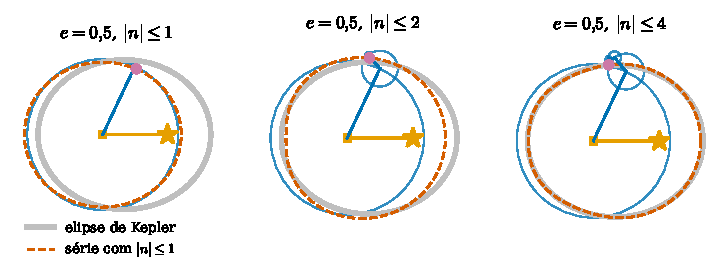
\includegraphics[width=\textwidth]{epiciclos.pdf}
  \legend{Em cinza, a elipse; tracejado, a série truncada em $|n|\leq N$. O segmento amarelo vai do Sol (estrela) ao termo fixo $c_0$; os círculos azuis são os epiciclos, montados em ordem decrescente de raio, e o ponto rosa é a ponta da cadeia no instante $t = 0{,}18\,T$. A excentricidade foi exagerada para tornar visíveis os epiciclos menores. Fonte: elaborada pelos autores.}
\end{figure}

\subsubsection{Da forma real para a complexa}

As duas formas carregam a mesma informação. Substituindo $\cos\theta = (e^{\ii\theta}+e^{-\ii\theta})/2$ e $\sin\theta = (e^{\ii\theta}-e^{-\ii\theta})/(2\ii)$ em $z = x + \ii y$, com $x$ e $y$ na forma \eqref{eq:fourier-real}, obtém-se para $n\geq1$
\begin{equation}
  c_{n} = \frac{(a_n + d_n) + \ii\,(c_n^{(y)} - b_n)}{2},
  \qquad
  c_{-n} = \frac{(a_n - d_n) + \ii\,(c_n^{(y)} + b_n)}{2},
  \label{eq:real-complexa}
\end{equation}
em que escrevemos $c_n^{(y)}$ para o coeficiente de cosseno de $y$, para não confundir com o coeficiente complexo. Os módulos
\[
  |c_n| = \tfrac12\sqrt{(a_n+d_n)^2 + (c_n^{(y)}-b_n)^2},\qquad
  |c_{-n}| = \tfrac12\sqrt{(a_n-d_n)^2 + (c_n^{(y)}+b_n)^2}
\]
são exatamente os raios $R_n$ e $r_n$ das equações 22 e 23 de \citeonline{farias2016}, que o TCC chamou de epiciclo de frequência $n\omega$ e epiciclo que gira em sentido contrário.

\begin{licao}[: senos e cossenos separados não são epiciclos]
As versões 1 e 2 do programa decompunham $x$ e $y$ separadamente, como na \autoref{eq:fourier-real}. Isso reconstrói a curva corretamente, mas um par $a_n\cos + b_n\sin$ em $x$ junto com $c_n\cos + d_n\sin$ em $y$ é uma \emph{elipse} alinhada aos eixos, e não um círculo. Para desenhar a cadeia histórica de epiciclos, a versão 3D passou a usar a série complexa, com $n$ percorrendo também os inteiros negativos. O TCC já fazia essa combinação ao calcular $R_n$ e $r_n$; o código levou duas versões para chegar lá.
\end{licao}

\subsection{A órbita de Kepler como função do tempo}\label{sec:param-tempo}

Para aplicar a \autoref{eq:fourier-complexa} a uma órbita é preciso escolher o parâmetro $t$. Há duas escolhas naturais, e elas \emph{não} são equivalentes:

\begin{itemize}
  \item \textbf{no tempo}: $z(t)$ é a posição do planeta no instante $t$. Pela segunda lei de Kepler, pontos igualmente espaçados no tempo ficam juntos perto do afélio, onde o planeta anda devagar, e espalhados perto do periélio (\autoref{fig:amostragem}a);
  \item \textbf{no ângulo}: $z(\theta) = r(\theta)e^{\ii\theta}$ é o ponto da elipse na direção $\theta$ vista do Sol, sem relação com o tempo (\autoref{fig:amostragem}b).
\end{itemize}

\begin{figure}[htb]
  \centering
  \caption{Trinta e seis pontos de uma mesma elipse ($e=0{,}5$) escolhidos de dois modos}
  \label{fig:amostragem}
  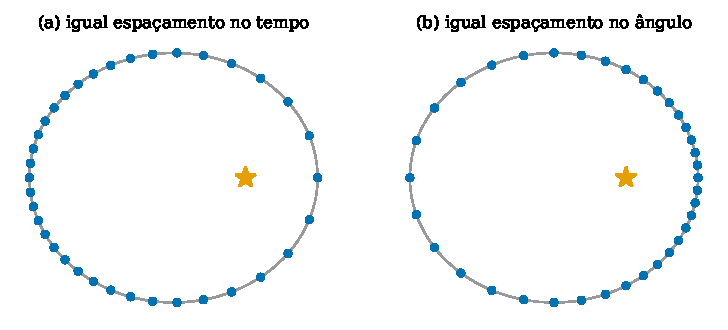
\includegraphics[width=0.85\textwidth]{amostragem.pdf}
  \legend{Em (a), cada ponto está a $T/36$ do seguinte, e o espaçamento desigual é a segunda lei de Kepler. Em (b), cada ponto está a $10^\circ$ do seguinte, visto do Sol (estrela). Fonte: elaborada pelos autores.}
\end{figure}

As duas são funções periódicas diferentes da mesma curva, com coeficientes diferentes. Só a parametrização no tempo tem significado físico: nela, ``girar com velocidade angular constante'' descreve o que um epiciclo faz \emph{no céu}, e é nela que o modelo de Copérnico pode ser comparado. A primeira versão do projeto amostrava em ângulo, e a \autoref{fig:angulo-tempo} mostra o efeito: para $e = 0{,}5$, o termo fixo vale $c_0 = -0{,}232\,a$ na amostragem em ângulo e $c_0 = -0{,}750\,a$ no tempo.

\begin{figure}[htb]
  \centering
  \caption{O mesmo cálculo de Fourier em duas parametrizações}
  \label{fig:angulo-tempo}
  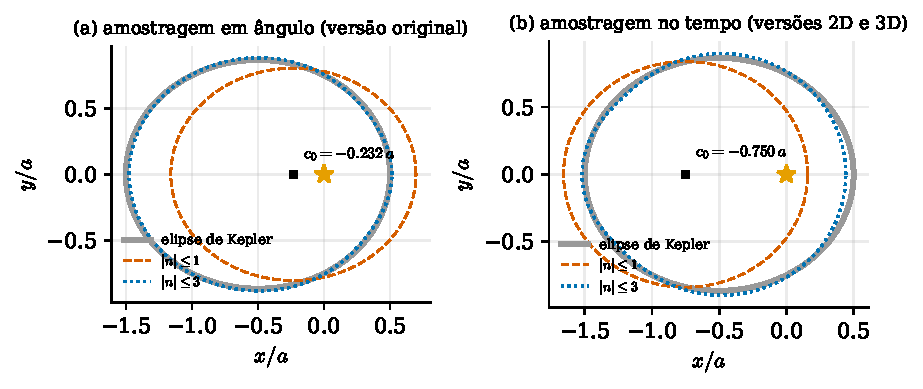
\includegraphics[width=0.95\textwidth]{angulo_tempo.pdf}
  \legend{Órbita hipotética com $e=0{,}5$. O quadrado preto marca $c_0$. As reconstruções com $|n|\leq1$ diferem: são aproximações de funções diferentes. Fonte: elaborada pelos autores.}
\end{figure}

\subsection{Os coeficientes em forma fechada}\label{sec:bessel}

Para a órbita kepleriana parametrizada no tempo, os coeficientes de Fourier têm forma fechada, escrita em termos das funções que Bessel estudou sistematicamente no início do século XIX, justamente no contexto do problema de Kepler \cite{watson1944,colwell1993}. Use a anomalia média $M = 2\pi t$ como variável e o periélio sobre o eixo real. Pela \autoref{eq:perifocal}, $z = a(\cos E - e) + \ii b\sin E$.

\subsubsection{O termo fixo}

Pela equação de Kepler, $\dd M = (1 - e\cos E)\,\dd E$. Então
\begin{align}
  c_0 = \frac{1}{2\pi}\int_0^{2\pi} z\,\dd M
  &= \frac{1}{2\pi}\int_0^{2\pi}\bigl[a(\cos E - e) + \ii b\sin E\bigr](1-e\cos E)\,\dd E \nonumber\\
  &= \frac{a}{2\pi}\int_0^{2\pi}\bigl(\cos E - e - e\cos^2E + e^2\cos E\bigr)\dd E \;+\; 0
   = a\Bigl(-e - \frac{e}{2}\Bigr),
\end{align}
porque $\cos E$ e $\sin E\cos E$ têm média nula e $\cos^2E$ tem média $\tfrac12$. Logo
\begin{equation}
  \boxed{\;c_0 = -\tfrac{3}{2}\,a e\;}
  \label{eq:c0}
\end{equation}
A posição média do planeta \emph{no tempo} fica a $\tfrac32 ae$ do Sol, do lado do afélio, e não a $ae$, que é onde está o centro geométrico da elipse. A diferença é a segunda lei: o planeta passa mais tempo longe do Sol, e a média temporal se desloca para lá.

\subsubsection{Os demais termos}

Para $n\neq0$, integra-se por partes e troca-se a variável para $E$; os detalhes estão no \autoref{ap:derivacoes}. Usando a representação integral de Bessel, $J_k(x) = \frac{1}{2\pi}\int_0^{2\pi}\cos(k\tau - x\sin\tau)\,\dd\tau$, chega-se a
\begin{equation}
  \boxed{\;c_n = \frac{a}{n}\,J_n'(ne) + \frac{b}{ne}\,J_n(ne),\qquad n\neq 0,\;}
  \label{eq:cn-bessel}
\end{equation}
válida para $n$ positivo e negativo, com $b = a\sqrt{1-e^2}$. Os coeficientes são todos reais: com o periélio no eixo real, a órbita é simétrica em relação a esse eixo. O \autoref{cap:resultados} confere a \autoref{eq:cn-bessel} contra os coeficientes calculados numericamente pelo programa; a diferença fica na casa de $10^{-16}$\,UA, o arredondamento da máquina.

\subsubsection{Desenvolvimento em pequena excentricidade}\label{sec:pequeno-e}

Para argumentos pequenos, $J_n(x)\approx (x/2)^n/n!$. Expandindo a \autoref{eq:cn-bessel} nas primeiras potências de $e$:
\begin{equation}
  c_0 = -\tfrac32 ae,\quad
  c_1 = a\Bigl(1-\tfrac{e^2}{2}\Bigr) + O(e^4),\quad
  c_2 = \tfrac12 ae + O(e^3),\quad
  c_{-1} = \tfrac18 ae^2 + O(e^4),
  \label{eq:pequeno-e}
\end{equation}
e todos os demais são de ordem $e^2$ ou superior. Portanto, até primeira ordem em $e$,
\begin{equation}
  \boxed{\;z(M) \;\approx\; -\tfrac32 ae \;+\; a\,e^{\ii M} \;+\; \tfrac12 ae\,e^{2\ii M}\;}
  \label{eq:copernico-fourier}
\end{equation}
A órbita de Kepler, vista como série de Fourier no tempo, é \emph{um deslocamento fixo, um deferente e um epiciclo que gira com o dobro da frequência}, com raios na razão $\tfrac32 : 1 : \tfrac12$ vezes $a$, $a$ e $ae$. O \autoref{sec:copernico-revisitado} mostra que essa é, termo a termo, a construção de Copérnico.

\subsection{Discretização: a série de Fourier no computador}\label{sec:dft}

No programa, a órbita entra como $A$ amostras igualmente espaçadas no tempo, $z_k = z(k/A)$, $k=0,\dots,A-1$, e a integral da \autoref{eq:fourier-complexa} vira a soma
\begin{equation}
  \hat c_n = \frac{1}{A}\sum_{k=0}^{A-1} z_k\,e^{-2\pi\ii nk/A},
  \label{eq:dft}
\end{equation}
a transformada discreta de Fourier (DFT) \cite{press2007}. A soma reproduz a integral exatamente para funções com espectro limitado, mas em geral cada coeficiente calculado é a soma de todos os coeficientes verdadeiros que coincidem com ele nas amostras: $\hat c_n = \sum_{m} c_{n+mA}$. Esse é o fenômeno de \emph{aliasing}. Ele impõe duas regras ao programa:

\begin{enumerate}
  \item com $A$ amostras, só os harmônicos com $|n| < A/2$ são recuperáveis (critério de Nyquist). O programa usa $A = 720$ e $|n|\leq 24$ e \emph{recusa}, com erro explícito, qualquer combinação que viole $2N < A$, em vez de devolver um número errado;
  \item mesmo dentro do limite, o erro depende de quão depressa $|c_n|$ decai. Para órbitas muito alongadas o espectro decai devagar, e a dobra dos termos altos contamina os baixos. Medido no programa, com 720 amostras: erro de coeficiente de $3\times10^{-16}$\,UA em $e = 0{,}6$, $10^{-14}$ em $e = 0{,}9$ e $10^{-8}$ em $e = 0{,}95$.
\end{enumerate}

O desvio da série truncada é medido ponto a ponto contra as próprias amostras. Pela identidade de Parseval, o desvio quadrático médio da série truncada em $|n|\leq N$ é $\bigl(\sum_{|n|>N}|c_n|^2\bigr)^{1/2}$: cada termo omitido contribui com o quadrado do próprio raio. É por isso que a convergência é tão rápida para órbitas quase circulares, em que os raios dos epiciclos caem como potências de $e$.

\subsection{Integração numérica}\label{sec:integradores}

\begin{paracomecar}
O computador não resolve a equação do movimento de uma vez. Ele dá passos: sabendo onde cada planeta está e com que velocidade, calcula onde estará meio dia depois, e repete. O problema é que os pequenos erros de cada passo se somam e, com o tempo, deformam a órbita.
\end{paracomecar}

\subsubsection{O problema de um método ingênuo}

O método mais simples, o de Euler, atualiza posição e velocidade usando os valores do início do passo: $\vr_{k+1} = \vr_k + \Delta t\,\vv_k$, $\vv_{k+1} = \vv_k + \Delta t\,\va(\vr_k)$. Para uma órbita circular, cada passo leva o corpo pela tangente, ligeiramente para fora do círculo, e a energia cresce a cada volta. Depois de algumas centenas de órbitas, o planeta escapa. Métodos de ordem mais alta, como o Runge--Kutta clássico de quarta ordem (RK4), erram muito menos em cada passo, mas o erro de energia continua tendo sinal sistemático e cresce sem limite, só que mais devagar.

\subsubsection{Integradores simpléticos}

As equações de Newton para a gravitação têm estrutura hamiltoniana: o estado é um ponto no espaço de fase $(\vr,\vv)$ e a evolução exata preserva volumes nesse espaço (teorema de Liouville). Um integrador \emph{simplético} é um método cujo passo também preserva essa estrutura \cite{hairer2006}. A consequência prática, demonstrada pela análise de erro regressiva, é que a solução numérica de um integrador simplético é a solução \emph{exata} de um hamiltoniano ligeiramente modificado, $\tilde H = H + O(\Delta t^p)$. Como $\tilde H$ se conserva exatamente, a energia verdadeira $H$ apenas oscila em torno do valor inicial, com amplitude $O(\Delta t^p)$, sem crescimento secular, por tempos exponencialmente longos.

\subsubsection{Leapfrog (Verlet)}

O integrador simplético mais simples é o \emph{leapfrog}, ou Verlet de velocidade \cite{verlet1967}. Ele alterna meio impulso, um deslocamento inteiro e outro meio impulso:
\begin{align}
  \vv_{k+1/2} &= \vv_k + \tfrac12\Delta t\,\va(\vr_k), \nonumber\\
  \vr_{k+1}   &= \vr_k + \Delta t\,\vv_{k+1/2}, \label{eq:leapfrog}\\
  \vv_{k+1}   &= \vv_{k+1/2} + \tfrac12\Delta t\,\va(\vr_{k+1}). \nonumber
\end{align}
É de segunda ordem, simétrico no tempo (dar um passo com $-\Delta t$ desfaz exatamente o passo com $+\Delta t$, a menos do arredondamento) e custa uma avaliação de força por passo, porque $\va(\vr_{k+1})$ é reaproveitada no passo seguinte. Denote por $S_2(\Delta t)$ esse passo.

\subsubsection{A composição de Yoshida}

\citeonline{yoshida1990} mostrou como construir métodos simpléticos de ordem mais alta compondo passos de um método simétrico de ordem 2. A versão de quarta ordem é
\begin{equation}
  S_4(\Delta t) = S_2(w_1\Delta t)\;S_2(w_0\Delta t)\;S_2(w_1\Delta t).
  \label{eq:yoshida}
\end{equation}
Os pesos saem de duas condições. A soma dos subpassos precisa dar o passo inteiro, $2w_1 + w_0 = 1$. E o termo de erro de terceira ordem, que em cada $S_2(h)$ é proporcional a $h^3$, precisa se cancelar: $2w_1^3 + w_0^3 = 0$. Resolvendo,
\begin{equation}
  w_1 = \frac{1}{2 - 2^{1/3}} \approx 1{,}35120719,\qquad
  w_0 = -\frac{2^{1/3}}{2 - 2^{1/3}} \approx -1{,}70241438.
  \label{eq:pesos-yoshida}
\end{equation}
O peso central é \emph{negativo}: o subpasso do meio anda para trás no tempo. O método resultante é simplético, simétrico, de quarta ordem e custa três avaliações de força por passo.

\begin{paraaprofundar}[: por que os pesos são escritos como números e não calculados]
O programa grava $w_1$ e $w_0$ como literais de 17 algarismos em vez de calcular $1/(2-\sqrt[3]{2})$ em tempo de execução. A razão é a reprodutibilidade: assim o valor não depende de a função de raiz cúbica de cada motor de JavaScript concordar com as demais no último bit. Um teste automatizado confere os literais contra a fórmula com tolerância de uma unidade na última casa.
\end{paraaprofundar}

\subsubsection{Passo fixo}

O simulador usa $S_4$ com passo \emph{fixo} de $\Delta t = 0{,}5$ dia, por duas razões independentes. Passo variável destrói a propriedade simplética, a menos de técnicas especiais. E com passo fixo a data exibida na tela é sempre exatamente $t_0 + k\cdot 0{,}5$ dia, sem arredondamento acumulado. O valor de meio dia foi escolhido por medição (\autoref{sec:res-integradores}).

\subsubsection{Interpolação para o desenho}

A física anda de meio em meio dia, mas a tela é redesenhada 60 ou 120 vezes por segundo. A 1 dia por segundo, isso daria dois saltos visíveis por segundo. O programa desenha uma posição intermediária entre dois estados integrados consecutivos usando a \emph{interpolação cúbica de Hermite}, que usa posição e velocidade nas duas pontas:
\begin{equation}
  \vr(\alpha) = h_{00}(\alpha)\,\vr_k + h_{10}(\alpha)\,\Delta t\,\vv_k + h_{01}(\alpha)\,\vr_{k+1} + h_{11}(\alpha)\,\Delta t\,\vv_{k+1},
  \qquad 0\le\alpha\le1,
  \label{eq:hermite}
\end{equation}
com $h_{00} = 2\alpha^3 - 3\alpha^2 + 1$, $h_{10} = \alpha^3 - 2\alpha^2 + \alpha$, $h_{01} = -2\alpha^3 + 3\alpha^2$ e $h_{11} = \alpha^3 - \alpha^2$. A curva resultante é contínua em posição e em velocidade nas fronteiras dos passos. Uma alternativa mais barata, extrapolar por Taylor a partir do estado atual, foi descartada por medição: em meio passo o termo de terceira ordem vale 213\,km em Mercúrio, 4\,\% do diâmetro do planeta, e isso aparecia como um tranco na fronteira de cada passo. A data escrita na tela é a do instante interpolado, $t_k + \alpha\Delta t$, de modo que o número na tela sempre corresponde ao desenho.

\subsection{Aritmética de ponto flutuante}\label{sec:float}

Computadores representam números reais com um número finito de algarismos binários, no padrão IEEE 754 \cite{ieee754,goldberg1991}. Em precisão dupla (\emph{float64}) há cerca de 16 algarismos decimais significativos; em precisão simples (\emph{float32}), cerca de 7. Toda a física do simulador roda em float64, e nessa precisão a posição de Netuno, a 30\,UA, fica quantizada em cerca de $10^{-15}\times 30\UA \approx 1\,\mathrm{mm}$.

As placas gráficas, porém, trabalham em float32, que em 30\,UA quantiza a centenas de quilômetros. O problema não é o valor em si, que seria invisível na tela, mas a \emph{subtração de dois números grandes e próximos}. A câmera a 30\,UA da origem olhando um planeta também a 30\,UA precisa calcular a diferença entre as duas posições, e em float32 essa diferença perde quase todos os algarismos significativos. A cena treme. A solução, descrita na \autoref{sec:origem-flutuante}, é fazer essa subtração em float64, na CPU, antes de enviar qualquer coisa para a placa.

\subsection{Escala de desenho}\label{sec:compressao}

Netuno está 77 vezes mais longe do Sol que Mercúrio. Numa tela que mostra o sistema inteiro em escala real, os quatro planetas internos ocupam uma área do tamanho de um dedo. O programa oferece, como opção desligada por padrão, o \emph{modo maquete}, que comprime as distâncias desenhadas por
\begin{equation}
  r_\text{desenho} = R\,\sqrt{r/R},\qquad R = 1\UA,
  \label{eq:compressao}
\end{equation}
preservando direções e mantendo a órbita da Terra inalterada (\autoref{fig:compressao}). A raiz foi preferida ao logaritmo porque é monótona, suave e vale zero em zero, enquanto o logaritmo leva o centro a $-\infty$ e exige um piso arbitrário. A razão entre o planeta mais distante e o mais próximo cai de 77:1 para 8,8:1.

\begin{figure}[htb]
  \centering
  \caption{A compressão de distâncias do modo maquete}
  \label{fig:compressao}
  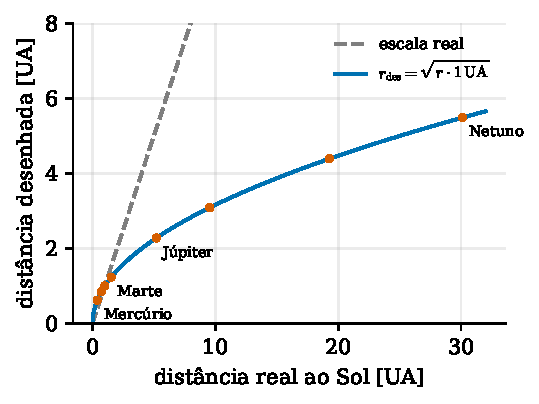
\includegraphics[width=0.62\textwidth]{compressao.pdf}
  \legend{Os pontos marcam os semieixos dos oito planetas. Fonte: elaborada pelos autores.}
\end{figure}

A compressão altera só a coordenada de desenho, nunca o estado físico. A iluminação continua usando a distância real, para que Netuno, desenhado a 5,5\,UA do Sol, não receba trinta vezes mais luz do que recebe. Com a compressão ligada, a tela avisa por escrito.

\section{Método: o simulador e sua validação}\label{sec:metodo}
% orçamento: 1.300 palavras

\subsection{Fundamentação física}\label{cap:fisica}

Este capítulo desenvolve a física que o simulador calcula. Partimos da lei da gravitação, escrevemos as equações de movimento de $N$ corpos e resolvemos o caso de dois corpos, que é o que dá as leis de Kepler e a linguagem dos elementos orbitais. As derivações seguem a linha de textos clássicos de mecânica e mecânica celeste \cite{symon1982,goldstein2002,murray1999,danby1988}. Algumas passagens mais longas estão no \autoref{ap:derivacoes}.

\subsubsection{Gravitação universal}

Dois corpos de massas $m_1$ e $m_2$, nas posições $\vr_1$ e $\vr_2$, atraem-se com força
\begin{equation}
  \vetor{F}_{12} = G\,\frac{m_1 m_2}{|\vr_2-\vr_1|^3}\,(\vr_2-\vr_1),
  \label{eq:newton}
\end{equation}
dirigida de um para o outro e proporcional ao inverso do quadrado da distância. Pela segunda lei de Newton, a aceleração do corpo 1 é $\va_1 = \vetor{F}_{12}/m_1$, e a massa $m_1$ se cancela: a aceleração que um corpo sofre não depende da própria massa, só da massa de quem o puxa.

\begin{paracomecar}
Uma pena e um martelo caem juntos na Lua, onde não há ar. Pela mesma razão, a Terra e um satélite artificial percorreriam a mesma órbita em torno do Sol se estivessem no mesmo lugar com a mesma velocidade.
\end{paracomecar}

\paragraph{Unidades e o parâmetro gravitacional}

Em mecânica celeste é mais conveniente trabalhar com o produto $GM$, o \emph{parâmetro gravitacional}, do que com $G$ e $M$ separados. O motivo é prático: $GM$ do Sol é conhecido com mais de dez algarismos significativos, porque é medido diretamente pelo movimento dos planetas e das sondas, enquanto $G$ é conhecido com apenas cerca de cinco \cite{park2021}. O simulador usa exclusivamente $GM$, em $\mathrm{UA^3/dia^2}$, com posições em unidades astronômicas ($1\UA = 149\,597\,870{,}7\km$) e tempo em dias. Nessas unidades, $GM_\odot \approx 2{,}959\times10^{-4}\,\mathrm{UA^3/dia^2}$, e os números das contas ficam todos numa faixa confortável para a aritmética de ponto flutuante.

\subsubsection{O problema de \texorpdfstring{$N$}{N} corpos}\label{sec:nbody}

Com $N$ corpos, cada um sente a soma das atrações de todos os outros:
\begin{equation}
  \ddot{\vr}_i \;=\; \sum_{\substack{j=1\\ j\neq i}}^{N} GM_j\,\frac{\vr_j-\vr_i}{|\vr_j-\vr_i|^3},
  \qquad i = 1,\dots,N.
  \label{eq:nbody}
\end{equation}
São $3N$ equações diferenciais de segunda ordem, acopladas. Para $N=2$ elas têm solução fechada (\autoref{sec:doiscorpos}). Para $N\geq 3$, em geral, não têm, e é preciso integrá-las numericamente (\autoref{sec:integradores}). O simulador integra $N=9$: o Sol e os oito planetas.

\paragraph{Grandezas conservadas}

Embora a \autoref{eq:nbody} não tenha solução geral, três grandezas permanecem constantes ao longo de qualquer solução exata, e por isso servem para medir a qualidade de uma solução numérica. Escrevendo $\mu_i = GM_i$:
\begin{align}
  \vetor{P} &= \sum_i \mu_i\,\dot{\vr}_i \quad\text{(momento linear, a menos do fator $1/G$)},\\
  \vetor{L} &= \sum_i \mu_i\,\vr_i\times\dot{\vr}_i \quad\text{(momento angular)},\\
  E &= \sum_i \tfrac12\mu_i\,|\dot{\vr}_i|^2 \;-\; \sum_{i<j}\frac{\mu_i\mu_j}{|\vr_i-\vr_j|} \quad\text{(energia)}.
  \label{eq:energia}
\end{align}
A conservação de $\vetor{P}$ implica que o centro de massa se move em linha reta com velocidade constante. Em particular, \emph{o Sol não fica parado}. Ele é puxado sobretudo por Júpiter e descreve em torno do centro de massa do sistema uma trajetória que chega a quase dois raios solares (\autoref{fig:sol-baricentro}, no \autoref{cap:resultados}).

\begin{paraaprofundar}[: por que a terceira lei economiza metade do trabalho]
Pela terceira lei de Newton, a força que $j$ exerce em $i$ é igual e oposta à que $i$ exerce em $j$. Na \autoref{eq:nbody} isso significa que o vetor $(\vr_j-\vr_i)/|\vr_j-\vr_i|^3$ é o mesmo, a menos do sinal, para os dois corpos do par. O código percorre cada par uma única vez, calcula esse vetor uma vez e o aplica aos dois, com pesos $GM_j$ e $-GM_i$. São $N(N-1)/2$ raízes quadradas em vez de $N(N-1)$ (\autoref{alg:forca}).
\end{paraaprofundar}

\subsubsection{O problema de dois corpos}\label{sec:doiscorpos}

Com apenas o Sol (massa $M$) e um planeta (massa $m$), subtraindo as duas equações de \eqref{eq:nbody} e chamando $\vr = \vr_\text{planeta}-\vr_\odot$ a posição \emph{relativa}, obtém-se
\begin{equation}
  \ddot{\vr} = -\mu\,\frac{\vr}{r^3},\qquad \mu = G(M+m).
  \label{eq:doiscorpos}
\end{equation}
O problema de dois corpos se reduz ao de um corpo só, atraído por um centro fixo com parâmetro $\mu$. Note que $\mu$ contém a soma das massas. Esse detalhe importa na \autoref{sec:elementos}.

\paragraph{Momento angular e a segunda lei de Kepler}

Defina o momento angular específico $\vh = \vr\times\dot{\vr}$. Derivando,
\[
  \dot{\vh} = \dot{\vr}\times\dot{\vr} + \vr\times\ddot{\vr} = \vetor{0} + \vr\times\Bigl(-\mu\frac{\vr}{r^3}\Bigr) = \vetor{0},
\]
porque o produto vetorial de um vetor consigo mesmo é nulo. Logo $\vh$ é constante. Duas consequências seguem imediatamente:

\begin{enumerate}
  \item $\vr$ é sempre perpendicular ao vetor fixo $\vh$, então o movimento acontece num plano;
  \item a área varrida pelo raio vetor num intervalo $\dd t$ é a de um triângulo de lados $\vr$ e $\dot{\vr}\,\dd t$, isto é, $\dd A = \tfrac12|\vr\times\dot{\vr}|\,\dd t$, de modo que
  \begin{equation}
    \frac{\dd A}{\dd t} = \frac{h}{2} = \text{constante}.
    \label{eq:segundalei}
  \end{equation}
\end{enumerate}
Essa é a segunda lei de Kepler, e ela vale para qualquer força central, não só para a gravitação.

\paragraph{O vetor de Laplace--Runge--Lenz e a primeira lei}\label{sec:lrl}

A força gravitacional tem uma simetria a mais que outras forças centrais, e ela se manifesta numa segunda grandeza conservada, o vetor excentricidade
\begin{equation}
  \ve = \frac{\dot{\vr}\times\vh}{\mu} - \frac{\vr}{r}.
  \label{eq:lrl}
\end{equation}
A verificação de que $\dot{\ve} = \vetor{0}$ é feita no \autoref{ap:derivacoes}. Supondo-a, faça o produto escalar de $\ve$ com $\vr$ e chame de $\nu$ o ângulo entre os dois:
\[
  \ve\cdot\vr = e\,r\cos\nu = \frac{\vr\cdot(\dot{\vr}\times\vh)}{\mu} - r = \frac{h^2}{\mu} - r,
\]
onde se usou $\vr\cdot(\dot{\vr}\times\vh) = (\vr\times\dot{\vr})\cdot\vh = h^2$. Isolando $r$:
\begin{equation}
  r(\nu) = \frac{h^2/\mu}{1 + e\cos\nu}.
  \label{eq:conica}
\end{equation}
É a equação de uma cônica em coordenadas polares com origem num foco. Para $e<1$ é uma elipse, a primeira lei de Kepler. O vetor $\ve$ aponta do foco para o periélio, e seu módulo é a excentricidade. O ângulo $\nu$, medido a partir do periélio, é a \emph{anomalia verdadeira}. Escrevendo o semilatus rectum como $p = h^2/\mu = a(1-e^2)$, recupera-se a forma $r = a(1-e^2)/(1+e\cos\nu)$ usada no TCC de \citeonline[Equação 16]{farias2016}.

\paragraph{Energia e a terceira lei}

A energia por unidade de massa, $\varepsilon = \tfrac12 v^2 - \mu/r$, também se conserva. Avaliando-a no periélio, onde $r = a(1-e)$ e $v = h/r$, chega-se a
\begin{equation}
  \varepsilon = -\frac{\mu}{2a}
  \qquad\Longleftrightarrow\qquad
  v^2 = \mu\Bigl(\frac{2}{r} - \frac{1}{a}\Bigr),
  \label{eq:visviva}
\end{equation}
a relação conhecida como \emph{vis-viva}. Ela diz que o semieixo maior depende apenas da energia: corpos com a mesma energia têm órbitas de mesmo tamanho, qualquer que seja a forma.

A terceira lei sai da segunda. Em um período $T$ o raio vetor varre a elipse inteira, de área $\pi ab$, com $b = a\sqrt{1-e^2}$. Pela \autoref{eq:segundalei}, $\pi ab = \tfrac12 h T$. Com $h = \sqrt{\mu p} = \sqrt{\mu a(1-e^2)}$,
\begin{equation}
  T = 2\pi\sqrt{\frac{a^3}{\mu}},
  \qquad\text{ou seja}\qquad
  n \equiv \frac{2\pi}{T} = \sqrt{\frac{\mu}{a^3}},
  \label{eq:terceiralei}
\end{equation}
onde $n$ é o \emph{movimento médio}, a velocidade angular média.

\subsubsection{Elementos orbitais}\label{sec:elementos}

Uma elipse no espaço, com o corpo situado sobre ela, fica determinada por seis números, os \emph{elementos keplerianos} (\autoref{fig:elementos}): dois dão a forma ($a$ e $e$), três dão a orientação no espaço ($i$, $\Omega$ e $\omega$) e um dá a posição do corpo sobre a órbita (a anomalia média $M$ numa época).

\begin{figure}[htb]
  \centering
  \caption{Os elementos orbitais}
  \label{fig:elementos}
  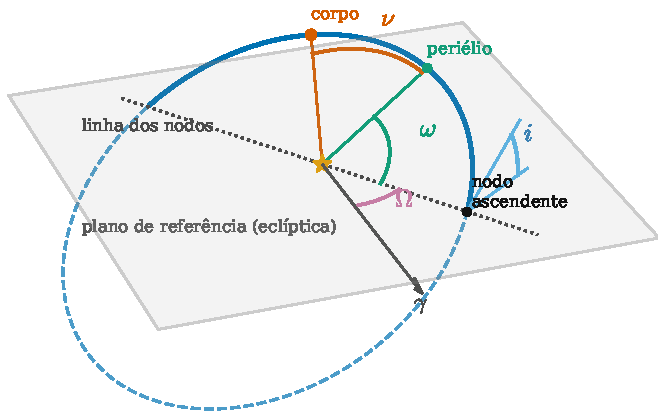
\includegraphics[width=0.85\textwidth]{elementos.pdf}
  \legend{$\Omega$: longitude do nodo ascendente, medida no plano de referência a partir da direção do equinócio $\gamma$; $i$: inclinação entre o plano da órbita e o de referência; $\omega$: argumento do periélio, medido no plano da órbita a partir do nodo; $\nu$: anomalia verdadeira. A parte tracejada da órbita está abaixo do plano de referência. O desenho é esquemático. Fonte: elaborada pelos autores.}
\end{figure}

Para levar um ponto da órbita ao espaço, escreve-se a posição na \emph{base perifocal}, com o eixo $x$ apontando para o periélio e o $y$ a $90^\circ$ no sentido do movimento, e aplica-se a rotação
\begin{equation}
  \vr = R_z(\Omega)\,R_x(i)\,R_z(\omega)\,
  \begin{pmatrix} x_P \\ y_P \\ 0 \end{pmatrix}.
  \label{eq:rotacao}
\end{equation}
A ordem importa. $R_z(\omega)$ gira o periélio a partir do nodo, $R_x(i)$ inclina o plano e $R_z(\Omega)$ leva o nodo à longitude certa. Trocar duas dessas rotações produz uma órbita plausível e errada, o tipo de erro que só aparece quando se compara com uma referência.

\paragraph{Elementos osculadores}

Num sistema real, a órbita de um planeta não é uma elipse fixa: os outros planetas a deformam devagar. Os \emph{elementos osculadores} num instante são os da elipse que o corpo seguiria se, a partir daquele instante, só o Sol existisse. Eles são calculados diretamente da posição e da velocidade relativas ao Sol:
\begin{align}
  a &= -\frac{\mu}{2\varepsilon} = \left(\frac{2}{r} - \frac{v^2}{\mu}\right)^{-1}, \label{eq:osc-a}\\
  \ve &= \frac{\vv\times\vh}{\mu} - \frac{\vr}{r}, \qquad e = |\ve|, \label{eq:osc-e}\\
  \cos i &= \frac{h_z}{|\vh|}, \label{eq:osc-i}
\end{align}
com $T$ dado pela \autoref{eq:terceiralei}. É o que o programa faz para desenhar o \emph{caminho previsto} de cada planeta e para alimentar o laboratório de Fourier.

\begin{licao}[: de onde se mede faz diferença]
A primeira versão do projeto (\autoref{sec:v-original}) calculava os elementos com a posição e a velocidade de cada planeta medidas a partir do \emph{baricentro} do Sistema Solar, que é o que a biblioteca Astropy devolve, mas usava nas fórmulas a gravidade do \emph{Sol}. As equações \eqref{eq:osc-a} a \eqref{eq:osc-i} valem para o estado \emph{relativo ao corpo central}. Como o Sol oscila em torno do baricentro cerca de 0,005 a 0,008\,UA, o erro era grande para os planetas internos: o semieixo de Mercúrio saía 1,7\,\% maior e a excentricidade de Vênus saía 0,0173 em vez de 0,0068, duas vezes e meia o valor correto. A correção é subtrair o estado do Sol antes de aplicar as fórmulas.
\end{licao}

\subsubsection{A equação de Kepler}\label{sec:kepler}

A segunda lei diz como a área varrida cresce com o tempo, mas não dá diretamente a posição em função do tempo. Para isso introduz-se a \emph{anomalia excêntrica} $E$, o ângulo medido do centro da elipse até a projeção do corpo sobre o círculo circunscrito de raio $a$ (\autoref{fig:anomalias}). Em termos de $E$, as coordenadas perifocais são
\begin{equation}
  x_P = a(\cos E - e),\qquad y_P = b\sin E = a\sqrt{1-e^2}\,\sin E,\qquad r = a(1 - e\cos E).
  \label{eq:perifocal}
\end{equation}

\begin{figure}[htb]
  \centering
  \caption{Anomalia excêntrica e anomalia verdadeira}
  \label{fig:anomalias}
  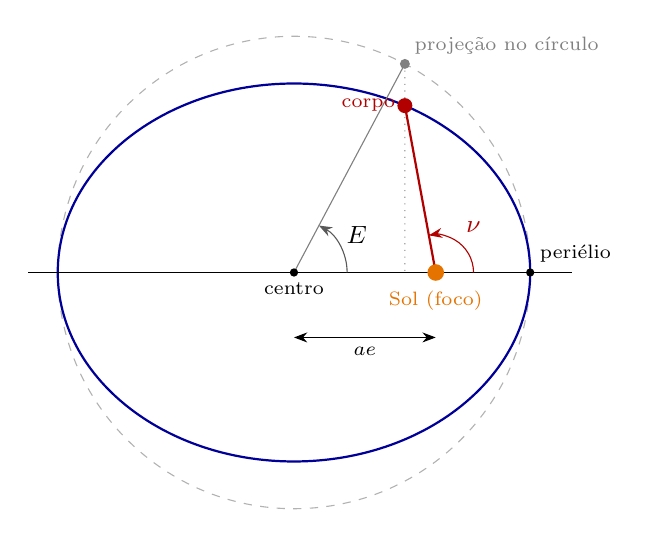
\begin{tikzpicture}[scale=1.5,>=Stealth]
    \def\semA{2.0}\def\exc{0.6}\def\angE{62}
    \pgfmathsetmacro{\semB}{\semA*sqrt(1-\exc*\exc)}
    \pgfmathsetmacro{\focC}{\semA*\exc}
    \pgfmathsetmacro{\angNu}{atan2(\semB*sin(\angE),\semA*cos(\angE)-\focC)}
    \coordinate (O) at (0,0);
    \coordinate (F) at (\focC,0);
    \coordinate (Q) at ({\semA*cos(\angE)},{\semA*sin(\angE)});
    \coordinate (P) at ({\semA*cos(\angE)},{\semB*sin(\angE)});
    \draw[gray!60,dashed] (O) circle (\semA);
    \draw[thick,blue!60!black] (O) ellipse ({\semA} and {\semB});
    \draw (-2.25,0) -- (2.35,0);
    \draw[gray] (O) -- (Q);
    \draw[gray,dotted] (Q) -- ({\semA*cos(\angE)},0);
    \draw[red!70!black,thick] (F) -- (P);
    \draw[->,gray!70!black] (0.45,0) arc (0:\angE:0.45);
    \node[font=\small] at ({0.62*cos(\angE/2)},{0.62*sin(\angE/2)}) {$E$};
    \draw[->,red!70!black] ($(F)+(0.32,0)$) arc (0:\angNu:0.32);
    \node[red!70!black,font=\small] at ($(F)+({0.5*cos(\angNu/2)},{0.5*sin(\angNu/2)})$) {$\nu$};
    \fill (O) circle (1pt) node[below,font=\scriptsize] {centro};
    \fill[orange!90!black] (F) circle (2pt) node[below=3pt,font=\scriptsize] {Sol (foco)};
    \fill[red!70!black] (P) circle (1.8pt) node[left,font=\scriptsize] {corpo};
    \fill[gray] (Q) circle (1.2pt) node[above right,font=\scriptsize] {projeção no círculo};
    \fill (\semA,0) circle (1pt) node[above right,font=\scriptsize] {periélio};
    \draw[<->] (0,-0.55) -- node[below,font=\scriptsize] {$ae$} (\focC,-0.55);
  \end{tikzpicture}
  \legend{O círculo tracejado tem raio $a$; a elipse é o círculo comprimido na vertical pelo fator $b/a$. Fonte: elaborada pelos autores.}
\end{figure}

A área do setor elíptico varrido desde o periélio, vista do foco, é a área do setor circular correspondente comprimida pelo fator $b/a$, menos o triângulo entre o centro e o foco:
\[
  A(E) = \frac{b}{a}\left(\frac{a^2E}{2} - \frac{a\cdot ae\,\sin E}{2}\right) = \frac{ab}{2}\,(E - e\sin E).
\]
Pela segunda lei, essa área cresce uniformemente no tempo e vale $\pi ab$ após um período. Logo $A = \pi ab\,(t-\tau)/T$, em que $\tau$ é o instante de passagem pelo periélio. Igualando as duas expressões e definindo a \emph{anomalia média} $M = n(t-\tau)$:
\begin{equation}
  \boxed{\;M = E - e\sin E\;}
  \label{eq:kepler}
\end{equation}
Esta é a equação de Kepler. Ela dá $M$ a partir de $E$ de forma explícita, mas o problema prático é o inverso: dado o tempo (e portanto $M$), achar $E$. Não há fórmula fechada com funções elementares, e a solução é numérica.

\paragraph{Solução pelo método de Newton}

Defina $f(E) = E - e\sin E - M$. O método de Newton itera
\begin{equation}
  E_{k+1} = E_k - \frac{f(E_k)}{f'(E_k)} = E_k - \frac{E_k - e\sin E_k - M}{1 - e\cos E_k}.
  \label{eq:newton-kepler}
\end{equation}
Para órbitas planetárias, com $e<0{,}21$, quatro ou cinco iterações a partir de $E_0 = M$ bastam para a precisão da máquina. O modo de criação de corpos do programa, porém, permite criar cometas com excentricidade próxima de 1, e nesse regime a escolha do ponto de partida importa. O programa usa o chute de \citeonline{danby1988},
\begin{equation}
  E_0 = M + 0{,}85\,e\,\sgn(\sin M),
\end{equation}
que coloca a primeira estimativa do lado certo do periélio. Como rede de segurança, se Newton não convergir o programa recorre à bisseção no intervalo $[M-e,\,M+e]$, que sempre contém a raiz porque $|E-M| = |e\sin E| \leq e$ e porque $f$ é monótona. A bisseção é lenta, mas nunca falha. O \autoref{cap:resultados} mede o número de iterações dos dois chutes (\autoref{fig:kepler-iteracoes}).

Com $E$ conhecido, a velocidade perifocal é
\begin{equation}
  \dot{x}_P = -\frac{\sqrt{\mu a}}{r}\sin E,\qquad \dot{y}_P = \frac{\sqrt{\mu a}}{r}\sqrt{1-e^2}\cos E,
\end{equation}
e a anomalia verdadeira, se necessária, sai da forma de meio ângulo
\[
  \tan\frac{\nu}{2} = \sqrt{\frac{1+e}{1-e}}\,\tan\frac{E}{2},
\]
calculada com a função \codigo{atan2} para não perder o quadrante.

\subsubsection{Referenciais e escala de tempo}

Todas as posições do simulador estão no referencial da eclíptica e equinócio de J2000, alinhado ao ICRF, com origem no baricentro do Sistema Solar \cite{park2021}. O tempo é o Tempo Dinâmico Baricêntrico (TDB), a variável independente das efemérides do JPL. A eclíptica de J2000 faz com o equador celeste o ângulo $\varepsilon_0 = 23{,}4392911^\circ$ (a obliquidade), usado para converter dados equatoriais, como os polos de rotação dos planetas publicados pela IAU \cite{archinal2018} e o catálogo de estrelas \cite{hoffleit1991}.

Os planetas são representados pelos \emph{baricentros dos seus sistemas}: o ponto chamado ``Terra'' é o centro de massa Terra--Lua, e o ponto ``Júpiter'' é o centro de massa de Júpiter com suas luas, cada um com a $GM$ do sistema inteiro. É assim que o próprio JPL integra os planetas, porque um sistema com luas se move, visto de longe, como um ponto de massa igual à soma das massas. O centro da Terra gira em torno do baricentro Terra--Lua a cerca de 4\,700\,km, o que na visão geral do sistema vale menos de um milésimo de pixel.

\subsubsection{O que o modelo físico não inclui}\label{sec:nao-inclui}

Ficam fora da integração:

\begin{itemize}
  \item a relatividade geral. O efeito mais conhecido é a precessão adicional do periélio de Mercúrio, de 43 segundos de arco por século \cite{will2018}. Em dez anos isso desloca o periélio de cerca de $2\times10^{-5}$\,rad, o que, multiplicado pela distância de Mercúrio ao Sol, dá da ordem de mil quilômetros. Esse valor é da ordem do patamar abaixo do qual o erro não cai ao reduzir o passo (\autoref{fig:trabalho-precisao}). Com o passo de 0,5 dia usado no programa, o erro de Mercúrio é maior que isso e vem sobretudo do truncamento do integrador;
  \item Plutão, os asteroides (inclusive Ceres e Vesta) e as luas como corpos dinâmicos separados;
  \item achatamento, marés e pressão de radiação.
\end{itemize}

Por isso os resultados se afastam devagar da efeméride do JPL, e o programa avisa o usuário. A versão 3D acrescenta treze luas, mas por outro método, sem integração (\autoref{sec:luas}).

% movido da seção 3 na Tarefa 6; a Tarefa 8 corta
\subsection{Integração numérica}\label{sec:integradores}

\begin{paracomecar}
O computador não resolve a equação do movimento de uma vez. Ele dá passos: sabendo onde cada planeta está e com que velocidade, calcula onde estará meio dia depois, e repete. O problema é que os pequenos erros de cada passo se somam e, com o tempo, deformam a órbita.
\end{paracomecar}

\subsubsection{O problema de um método ingênuo}

O método mais simples, o de Euler, atualiza posição e velocidade usando os valores do início do passo: $\vr_{k+1} = \vr_k + \Delta t\,\vv_k$, $\vv_{k+1} = \vv_k + \Delta t\,\va(\vr_k)$. Para uma órbita circular, cada passo leva o corpo pela tangente, ligeiramente para fora do círculo, e a energia cresce a cada volta. Depois de algumas centenas de órbitas, o planeta escapa. Métodos de ordem mais alta, como o Runge--Kutta clássico de quarta ordem (RK4), erram muito menos em cada passo, mas o erro de energia continua tendo sinal sistemático e cresce sem limite, só que mais devagar.

\subsubsection{Integradores simpléticos}

As equações de Newton para a gravitação têm estrutura hamiltoniana: o estado é um ponto no espaço de fase $(\vr,\vv)$ e a evolução exata preserva volumes nesse espaço (teorema de Liouville). Um integrador \emph{simplético} é um método cujo passo também preserva essa estrutura \cite{hairer2006}. A consequência prática, demonstrada pela análise de erro regressiva, é que a solução numérica de um integrador simplético é a solução \emph{exata} de um hamiltoniano ligeiramente modificado, $\tilde H = H + O(\Delta t^p)$. Como $\tilde H$ se conserva exatamente, a energia verdadeira $H$ apenas oscila em torno do valor inicial, com amplitude $O(\Delta t^p)$, sem crescimento secular, por tempos exponencialmente longos.

\subsubsection{Leapfrog (Verlet)}

O integrador simplético mais simples é o \emph{leapfrog}, ou Verlet de velocidade \cite{verlet1967}. Ele alterna meio impulso, um deslocamento inteiro e outro meio impulso:
\begin{align}
  \vv_{k+1/2} &= \vv_k + \tfrac12\Delta t\,\va(\vr_k), \nonumber\\
  \vr_{k+1}   &= \vr_k + \Delta t\,\vv_{k+1/2}, \label{eq:leapfrog}\\
  \vv_{k+1}   &= \vv_{k+1/2} + \tfrac12\Delta t\,\va(\vr_{k+1}). \nonumber
\end{align}
É de segunda ordem, simétrico no tempo (dar um passo com $-\Delta t$ desfaz exatamente o passo com $+\Delta t$, a menos do arredondamento) e custa uma avaliação de força por passo, porque $\va(\vr_{k+1})$ pode ser reaproveitada no passo seguinte. O simulador não faz esse reaproveitamento e gasta duas avaliações; nas comparações de custo da \autoref{sec:res-integradores} contamos uma, que é o custo do método. Denote por $S_2(\Delta t)$ esse passo.

\subsubsection{A composição de Yoshida}

\citeonline{yoshida1990} mostrou como construir métodos simpléticos de ordem mais alta compondo passos de um método simétrico de ordem 2. A versão de quarta ordem é
\begin{equation}
  S_4(\Delta t) = S_2(w_1\Delta t)\;S_2(w_0\Delta t)\;S_2(w_1\Delta t).
  \label{eq:yoshida}
\end{equation}
Os pesos saem de duas condições. A soma dos subpassos precisa dar o passo inteiro, $2w_1 + w_0 = 1$. E o termo de erro de terceira ordem, que em cada $S_2(h)$ é proporcional a $h^3$, precisa se cancelar: $2w_1^3 + w_0^3 = 0$. Resolvendo,
\begin{equation}
  w_1 = \frac{1}{2 - 2^{1/3}} \approx 1{,}35120719,\qquad
  w_0 = -\frac{2^{1/3}}{2 - 2^{1/3}} \approx -1{,}70241438.
  \label{eq:pesos-yoshida}
\end{equation}
O peso central é \emph{negativo}: o subpasso do meio anda para trás no tempo. O método resultante é simplético, simétrico, de quarta ordem e custa três avaliações de força por passo.

\begin{paraaprofundar}[: por que os pesos são escritos como números e não calculados]
O programa grava $w_1$ e $w_0$ como literais de 17 algarismos em vez de calcular $1/(2-\sqrt[3]{2})$ em tempo de execução. A razão é a reprodutibilidade: assim o valor não depende de a função de raiz cúbica de cada motor de JavaScript concordar com as demais no último bit. Um teste automatizado confere os literais contra a fórmula com tolerância de uma unidade na última casa.
\end{paraaprofundar}

\subsubsection{Passo fixo}

O simulador usa $S_4$ com passo \emph{fixo} de $\Delta t = 0{,}5$ dia, por duas razões independentes. Passo variável destrói a propriedade simplética, a menos de técnicas especiais. E com passo fixo a data exibida na tela é sempre exatamente $t_0 + k\cdot 0{,}5$ dia, sem arredondamento acumulado. O valor de meio dia foi escolhido por medição (\autoref{sec:res-integradores}).

\subsubsection{Interpolação para o desenho}

A física anda de meio em meio dia, mas a tela é redesenhada 60 ou 120 vezes por segundo. A 1 dia por segundo, isso daria dois saltos visíveis por segundo. O programa desenha uma posição intermediária entre dois estados integrados consecutivos usando a \emph{interpolação cúbica de Hermite}, que usa posição e velocidade nas duas pontas:
\begin{equation}
  \vr(\alpha) = h_{00}(\alpha)\,\vr_k + h_{10}(\alpha)\,\Delta t\,\vv_k + h_{01}(\alpha)\,\vr_{k+1} + h_{11}(\alpha)\,\Delta t\,\vv_{k+1},
  \qquad 0\le\alpha\le1,
  \label{eq:hermite}
\end{equation}
com $h_{00} = 2\alpha^3 - 3\alpha^2 + 1$, $h_{10} = \alpha^3 - 2\alpha^2 + \alpha$, $h_{01} = -2\alpha^3 + 3\alpha^2$ e $h_{11} = \alpha^3 - \alpha^2$. A curva resultante é contínua em posição e em velocidade nas fronteiras dos passos. Uma alternativa mais barata, extrapolar por Taylor a partir do estado atual, foi descartada por medição: em meio passo o termo de terceira ordem vale 213\,km em Mercúrio, 4\,\% do diâmetro do planeta, e isso aparecia como um tranco na fronteira de cada passo. A data escrita na tela é a do instante interpolado, $t_k + \alpha\Delta t$, de modo que o número na tela sempre corresponde ao desenho.

\subsection{Aritmética de ponto flutuante}\label{sec:float}

Computadores representam números reais com um número finito de algarismos binários, no padrão IEEE 754 \cite{ieee754,goldberg1991}. Em precisão dupla (\emph{float64}) há cerca de 16 algarismos decimais significativos; em precisão simples (\emph{float32}), cerca de 7. Toda a física do simulador roda em float64, e nessa precisão a posição de Netuno, a 30\,UA, fica quantizada em cerca de $10^{-15}\times 30\UA \approx 1\,\mathrm{mm}$.

As placas gráficas, porém, trabalham em float32, que em 30\,UA quantiza a centenas de quilômetros. O problema não é o valor em si, que seria invisível na tela, mas a \emph{subtração de dois números grandes e próximos}. A câmera a 30\,UA da origem olhando um planeta também a 30\,UA precisa calcular a diferença entre as duas posições, e em float32 essa diferença perde quase todos os algarismos significativos. A cena treme. A solução, descrita na \autoref{sec:origem-flutuante}, é fazer essa subtração em float64, na CPU, antes de enviar qualquer coisa para a placa.

\subsection{Escala de desenho}\label{sec:compressao}

Netuno está 77 vezes mais longe do Sol que Mercúrio. Numa tela que mostra o sistema inteiro em escala real, os quatro planetas internos ocupam uma área do tamanho de um dedo. O programa oferece, como opção desligada por padrão, o \emph{modo maquete}, que comprime as distâncias desenhadas por
\begin{equation}
  r_\text{desenho} = R\,\sqrt{r/R},\qquad R = 1\UA,
  \label{eq:compressao}
\end{equation}
preservando direções e mantendo a órbita da Terra inalterada (\autoref{fig:compressao}). A raiz foi preferida ao logaritmo porque é monótona, suave e vale zero em zero, enquanto o logaritmo leva o centro a $-\infty$ e exige um piso arbitrário. A razão entre o planeta mais distante e o mais próximo cai de 77:1 para 8,8:1.

\begin{figure}[htb]
  \centering
  \caption{A compressão de distâncias do modo maquete}
  \label{fig:compressao}
  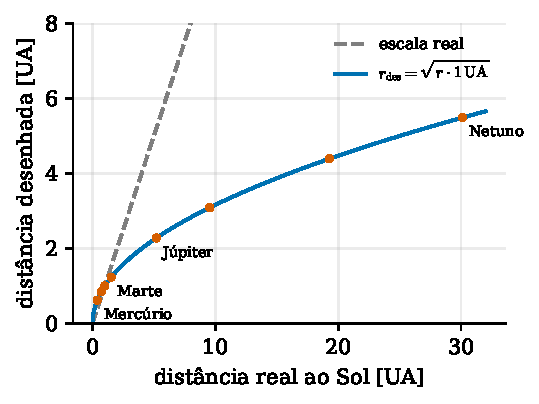
\includegraphics[width=0.62\textwidth]{compressao.pdf}
  \legend{Os pontos marcam os semieixos dos oito planetas. Fonte: elaborada pelos autores.}
\end{figure}

A compressão altera só a coordenada de desenho, nunca o estado físico. A iluminação continua usando a distância real, para que Netuno, desenhado a 5,5\,UA do Sol, não receba trinta vezes mais luz do que recebe. Com a compressão ligada, a tela avisa por escrito.

\subsection{Implementação: três gerações de um mesmo programa}\label{cap:implementacao}

O projeto passou por três versões, cada uma nascida das limitações da anterior (\autoref{fig:linha-do-tempo}). Este capítulo descreve o que cada uma fez, como a física e a matemática dos capítulos anteriores viraram código e por que algumas decisões foram tomadas. Os algoritmos aparecem em pseudocódigo; o código real está no repositório indicado no \autoref{ap:reproducao}.

\begin{figure}[htb]
  \centering
  \caption{As três gerações do projeto}
  \label{fig:linha-do-tempo}
  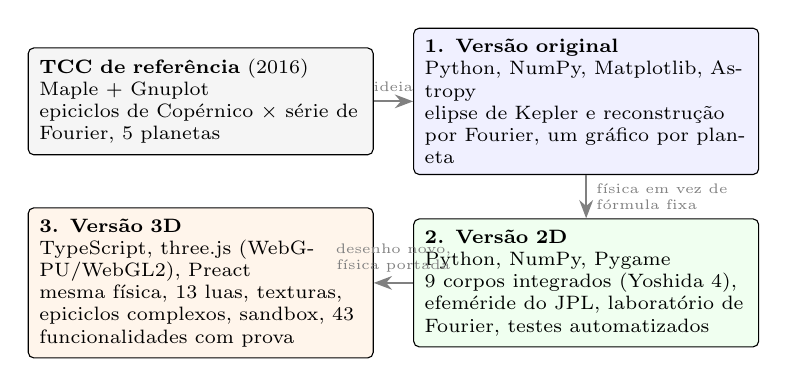
\begin{tikzpicture}[
      node distance=0.55cm and 0.5cm,
      caixa/.style={draw,rounded corners=2pt,align=left,font=\scriptsize,text width=4.1cm,inner sep=4pt},
      titulo/.style={font=\small\bfseries,align=center},
      >=Stealth]
    \node[caixa,fill=gray!8] (tcc) {\textbf{TCC de referência} (2016)\\ Maple + Gnuplot\\ epiciclos de Copérnico $\times$ série de Fourier, 5 planetas};
    \node[caixa,fill=blue!6,right=of tcc] (v1) {\textbf{1. Versão original}\\ Python, NumPy, Matplotlib, Astropy\\ elipse de Kepler e reconstrução por Fourier, um gráfico por planeta};
    \node[caixa,fill=green!6,below=of v1] (v2) {\textbf{2. Versão 2D}\\ Python, NumPy, Pygame\\ 9 corpos integrados (Yoshida 4), efeméride do JPL, laboratório de Fourier, testes automatizados};
    \node[caixa,fill=orange!8,left=of v2] (v3) {\textbf{3. Versão 3D}\\ TypeScript, three.js (WebGPU/WebGL2), Preact\\ mesma física, 13 luas, texturas, epiciclos complexos, sandbox, 43 funcionalidades com prova};
    \draw[->,thick,gray] (tcc) -- node[above,font=\tiny]{ideia} (v1);
    \draw[->,thick,gray] (v1) -- node[right,font=\tiny,align=left]{física em vez de\\fórmula fixa} (v2);
    \draw[->,thick,gray] (v2) -- node[above,font=\tiny,align=center]{desenho novo,\\física portada} (v3);
  \end{tikzpicture}
  \legend{Fonte: elaborada pelos autores.}
\end{figure}

\subsubsection{Versão original: a elipse e a série}\label{sec:v-original}

A primeira versão, em Python, tem cerca de 300 linhas e faz uma coisa só: dado um planeta e um número de termos, desenha a elipse de Kepler e a aproximação por série de Fourier no mesmo gráfico do Matplotlib. Ela reproduz, com ferramentas modernas, o experimento numérico de \citeonline{farias2016}.

O passo que essa versão acrescentou ao TCC foi obter os elementos orbitais de uma efeméride em vez de copiá-los de uma tabela. A biblioteca Astropy \cite{astropy2022} fornece posição e velocidade de cada planeta na época J2000, e as equações \eqref{eq:osc-a} a \eqref{eq:osc-i} dão $a$, $e$ e $T$. Foi aqui que apareceu o erro de referencial descrito na lição do \autoref{sec:elementos}: os vetores vinham do baricentro, e a excentricidade de Vênus saía duas vezes e meia maior que a real. A \autoref{tab:v1-baricentro} mostra o efeito, medido no próprio código depois da correção.

\begin{table}[htb]
  \centering
  \caption{Elementos calculados na versão original, antes e depois da correção de referencial}
  \label{tab:v1-baricentro}
  \begin{tabular}{lccc}
    \toprule
    Planeta & $a$ com vetores baricêntricos (UA) & $a$ corrigido (UA) & referência (UA) \\
    \midrule
    Mercúrio & 0,39378 \;(+1,73\,\%) & 0,38710 & 0,38710 \\
    Vênus    & 0,73868 \;(+2,12\,\%) & 0,72332 & 0,72333 \\
    Terra    & 0,99657 \;($-$0,34\,\%) & 1,00000 & 1,00000 \\
    Marte    & 1,50514 \;($-$1,22\,\%) & 1,52376 & 1,52371 \\
    \bottomrule
  \end{tabular}
  \legend{Época J2000, efeméride embutida do Astropy. A excentricidade de Vênus passou de 0,01734 para 0,00677. Fonte: documentação do módulo \arquivo{utils/lib.py} da versão original.}
\end{table}

Essa versão também amostrava a elipse \emph{em ângulo}, e não no tempo, o que, como vimos no \autoref{sec:param-tempo}, dá coeficientes de outra função. Ela permanece no repositório como referência científica e como registro do ponto de partida.

\subsubsection{Versão 2D: a física no lugar da fórmula}\label{sec:v2d}

A segunda versão deixou de desenhar uma elipse a partir de uma fórmula e passou a \emph{simular} o Sistema Solar: o Sol e os oito planetas se atraem mutuamente pela \autoref{eq:nbody}, todos no mesmo relógio, a partir das posições e velocidades medidas pelo JPL para 1º de janeiro de 2026. A elipse passou a ser uma consequência da simulação: ao abrir o laboratório de Fourier, o programa calcula os elementos osculadores do planeta naquele instante e a decompõe.

\begin{figure}[htb]
  \centering
  \caption{A versão 2D, em Python e Pygame}
  \label{fig:v2}
  \begin{subfigure}[b]{0.49\textwidth}
    \centering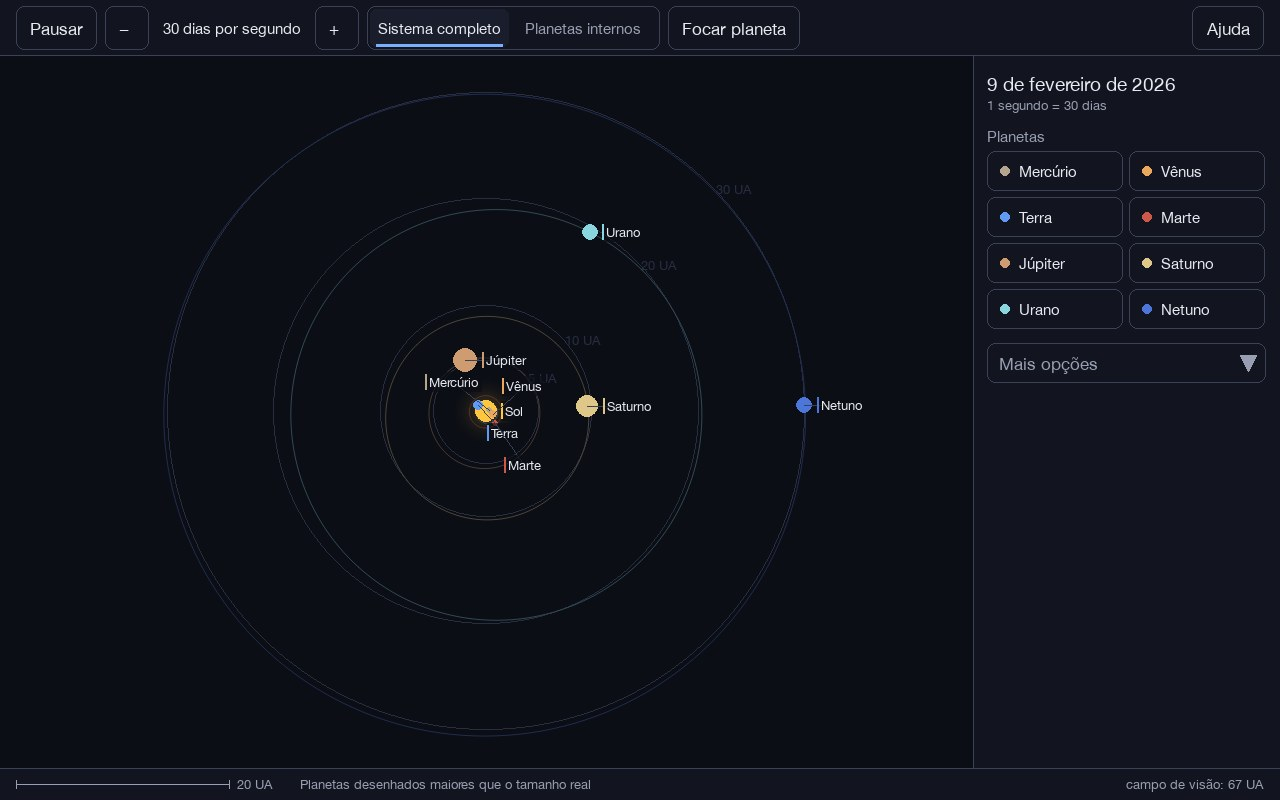
\includegraphics[width=\textwidth]{v2_visao_geral.jpg}
    \caption{Visão geral, em escala real}
  \end{subfigure}\hfill
  \begin{subfigure}[b]{0.49\textwidth}
    \centering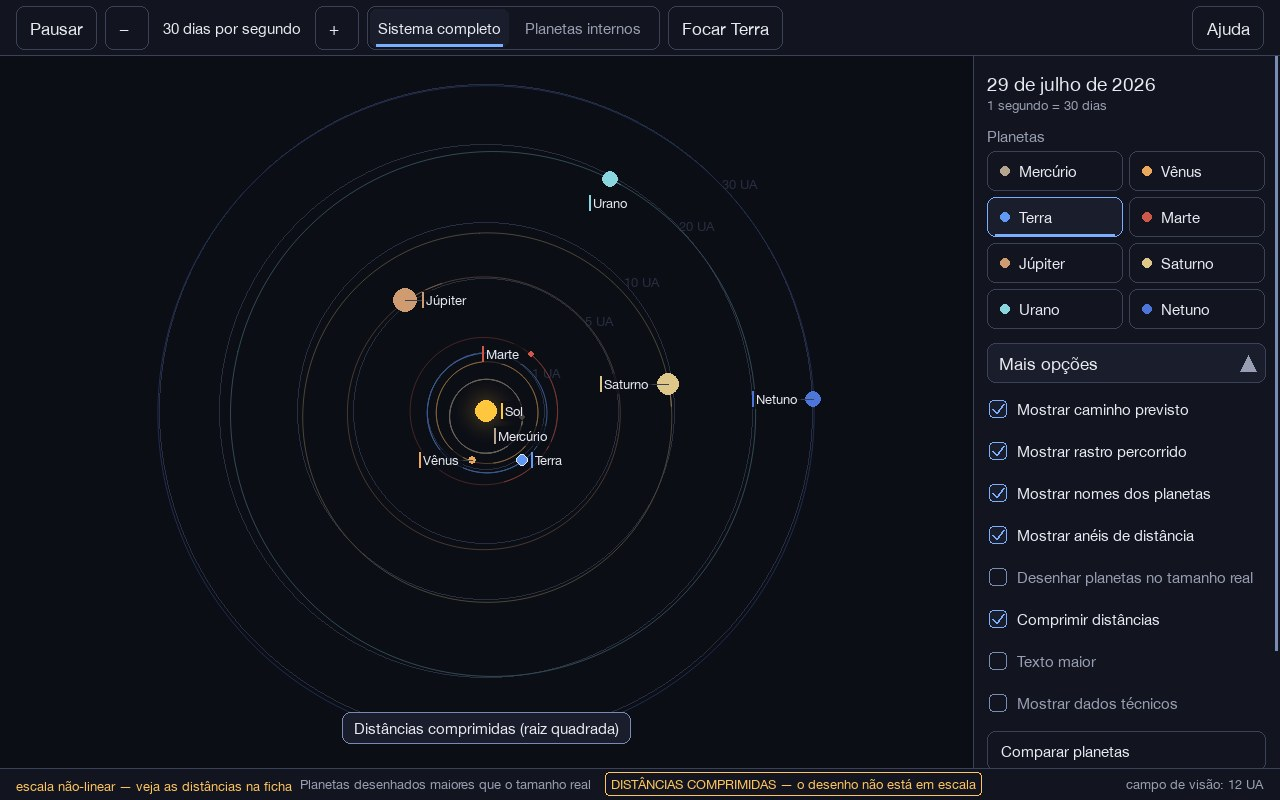
\includegraphics[width=\textwidth]{v2_comprimida.jpg}
    \caption{Com distâncias comprimidas}
  \end{subfigure}\\[4pt]
  \begin{subfigure}[b]{0.49\textwidth}
    \centering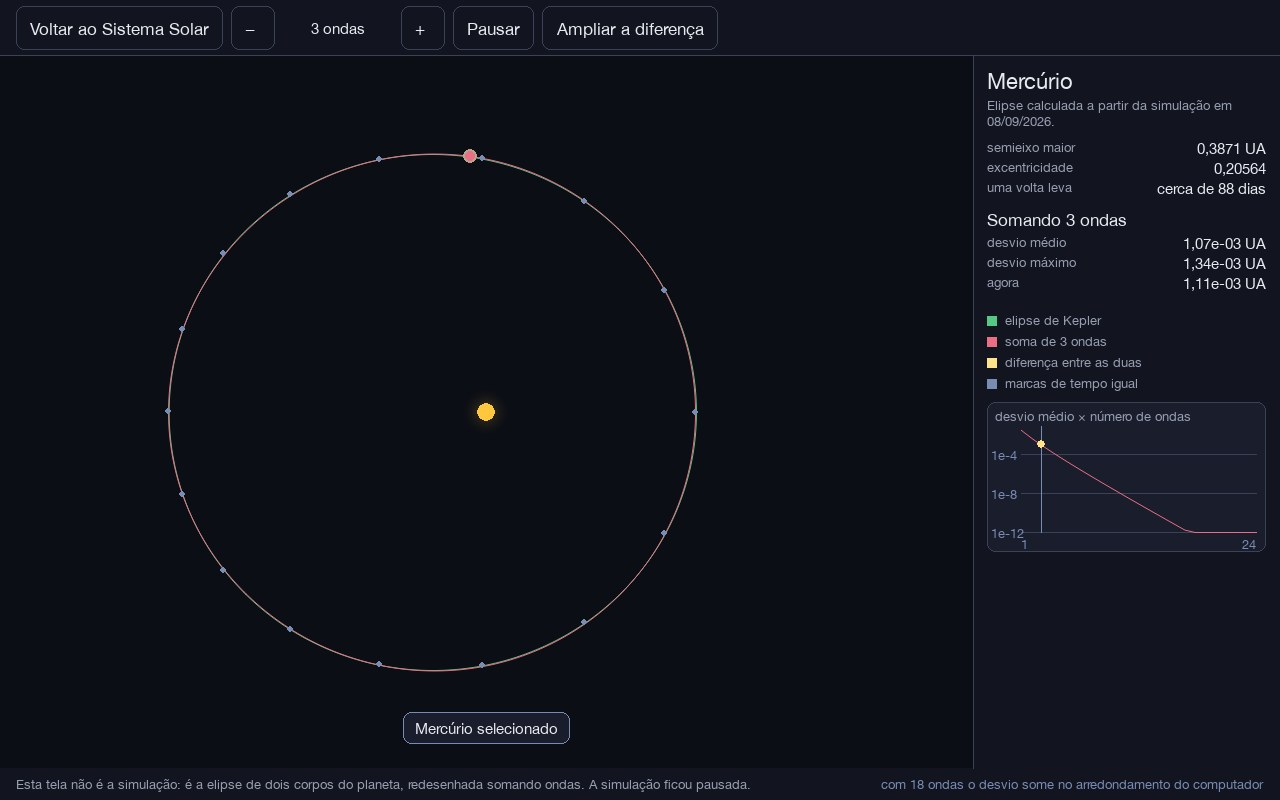
\includegraphics[width=\textwidth]{v2_laboratorio.jpg}
    \caption{Laboratório: Mercúrio com 3 ondas}
  \end{subfigure}\hfill
  \begin{subfigure}[b]{0.49\textwidth}
    \centering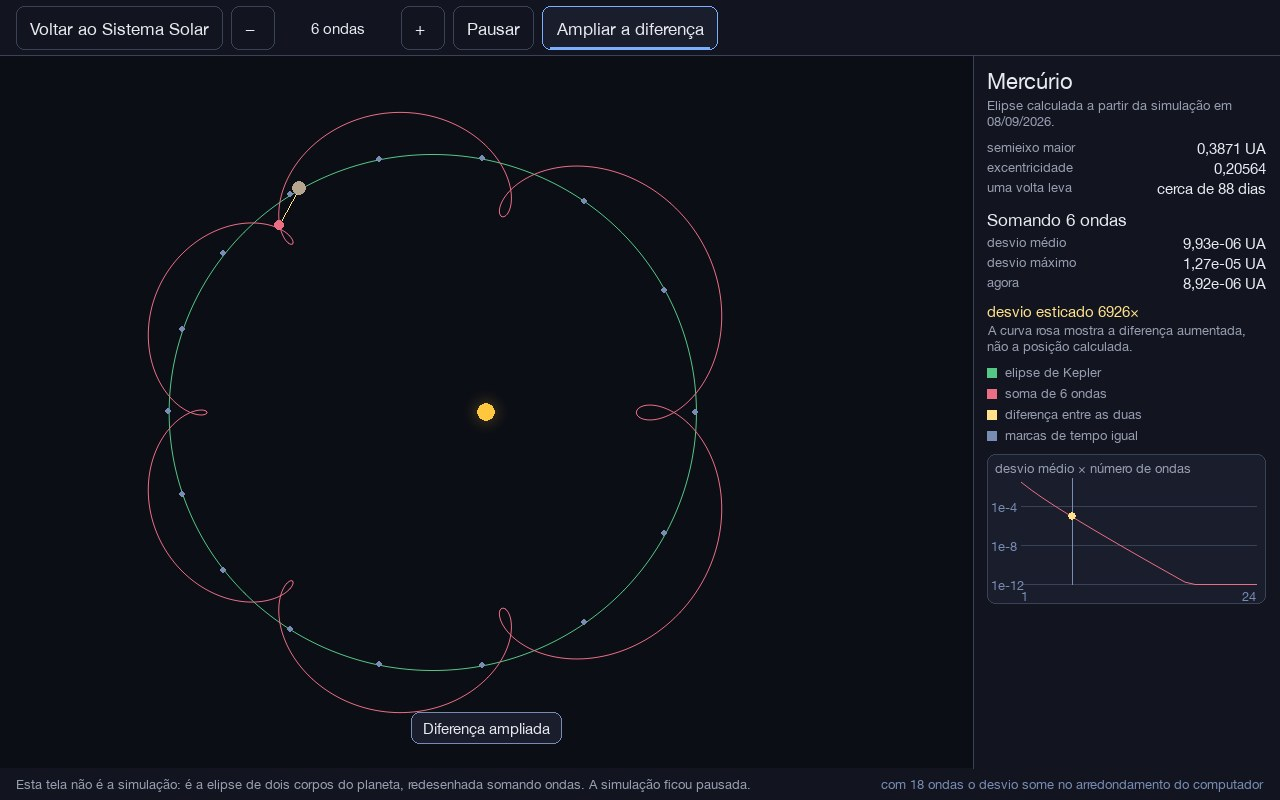
\includegraphics[width=\textwidth]{v2_laboratorio_ampliado.jpg}
    \caption{Diferença ampliada 6\,926 vezes}
  \end{subfigure}
  \legend{Em (b) a tela avisa por escrito que o desenho não está em escala. Em (d) a curva rosa mostra a diferença entre a série com 6 ondas e a elipse, multiplicada para ficar visível; o gráfico à direita mostra a convergência. Fonte: capturas do programa.}
\end{figure}

\paragraph{Dados de partida}

Um roteiro separado, \arquivo{ferramentas/gerar\_efemeride.py}, consulta uma única vez a API do JPL Horizons \cite{giorgini1996} e grava num arquivo JSON:

\begin{itemize}
  \item posição e velocidade de cada corpo em 1/1/2026, 0h TDB, relativas ao baricentro do Sistema Solar, no referencial da eclíptica J2000 (o Horizons informa a efeméride DE441 como origem);
  \item os parâmetros gravitacionais $GM$ do cabeçalho da efeméride DE440 \cite{park2021};
  \item os raios médios dos corpos;
  \item posições de validação em $-100$, $-10$, $+1$, $+10$ e $+100$ anos, que os testes usam para medir o erro;
  \item a procedência de cada número.
\end{itemize}

O programa em si \emph{nunca acessa a internet}: o arquivo é copiado junto. A versão 3D usa o mesmo arquivo, byte a byte, o que mantém válida a mesma tabela de erro.

\paragraph{Integração e relógio}

O integrador é o Yoshida de quarta ordem com passo fixo de 0,5 dia (\autoref{sec:integradores}), com o leapfrog mantido como referência independente nos testes. A força é calculada pelo \autoref{alg:forca} e o passo pelo \autoref{alg:yoshida}.

\begin{algorithm}[htb]
  \caption{Aceleração gravitacional mútua de $N$ corpos}\label{alg:forca}
  \KwIn{posições $\vr_1,\dots,\vr_N$ e parâmetros $\mu_1,\dots,\mu_N$}
  \KwOut{acelerações $\va_1,\dots,\va_N$}
  $\va_i \leftarrow \vetor{0}$ para todo $i$\;
  \For{$i\leftarrow 1$ \KwTo $N-1$}{
    \For{$j\leftarrow i+1$ \KwTo $N$}{
      $\vetor{d} \leftarrow \vr_j - \vr_i$;\quad $s \leftarrow 1/(|\vetor{d}|^2\,|\vetor{d}|)$\Com*[r]{uma raiz por par}
      $\va_i \leftarrow \va_i + \mu_j\, s\,\vetor{d}$\Com*[r]{$j$ puxa $i$}
      $\va_j \leftarrow \va_j - \mu_i\, s\,\vetor{d}$\Com*[r]{terceira lei}
    }
  }
\end{algorithm}

\begin{algorithm}[htb]
  \caption{Um passo de Yoshida de quarta ordem}\label{alg:yoshida}
  \KwIn{estado $(\vr,\vv)$, passo $\Delta t$}
  $w_1 \leftarrow 1{,}3512071919596578$;\quad $w_0 \leftarrow -1{,}7024143839193155$\;
  \ForEach{$w \in (w_1, w_0, w_1)$}{
    $\vr \leftarrow \vr + \tfrac12 w\,\Delta t\,\vv$\Com*[r]{meio deslocamento}
    $\va \leftarrow$ \textsc{Aceleração}$(\vr)$\Com*[r]{\autoref{alg:forca}}
    $\vv \leftarrow \vv + w\,\Delta t\,\va$\Com*[r]{impulso}
    $\vr \leftarrow \vr + \tfrac12 w\,\Delta t\,\vv$\Com*[r]{meio deslocamento}
  }
\end{algorithm}

Quando a pessoa pede, por exemplo, 3\,650 dias simulados por segundo, cada quadro de tela precisa de dezenas de passos. Se a máquina não der conta, há três saídas ruins: aumentar o passo (a física piora sem aviso), acumular a dívida (o programa trava tentando alcançar) ou pular passos (a data na tela deixa de corresponder ao desenho). O simulador mede a velocidade da máquina na abertura, oferece só as velocidades que ela sustenta, entrega em cada quadro os passos que cabem no orçamento, \emph{descarta} o excedente e avisa na tela que está atrasado (\autoref{alg:relogio}). A data mostrada é sempre $t_0 + k\cdot0{,}5$ dia exatos.

\begin{algorithm}[htb]
  \caption{Avanço do relógio dentro do orçamento do quadro (simplificado)}\label{alg:relogio}
  \KwIn{tempo real decorrido $\delta$, velocidade pedida $s$ (dias/segundo), orçamento $B$ (ms), cronômetro injetado}
  $\text{dívida} \leftarrow \text{dívida} + s\,\delta$\;
  $k \leftarrow 0$;\quad $t_\text{ini} \leftarrow$ cronômetro()\;
  \While{$\text{dívida} \geq \Delta t$ \textbf{e} cronômetro()$ - t_\text{ini} < B$}{
    \textsc{PassoYoshida}$(\Delta t)$;\quad $\text{dívida} \leftarrow \text{dívida} - \Delta t$;\quad $k \leftarrow k+1$\;
  }
  \If{$\text{dívida} \geq \Delta t$}{
    $\text{atrasado} \leftarrow$ verdadeiro;\quad $\text{dívida} \leftarrow \text{dívida} \bmod \Delta t$\Com*[r]{descarta, não acumula}
  }
  \Return $k$ passos dados, atrasado\;
\end{algorithm}

\paragraph{Laboratório de Fourier}

O laboratório pausa a simulação, calcula os elementos osculadores do corpo escolhido, gera a elipse de Kepler com 720 pontos igualmente espaçados no tempo (resolvendo a equação de Kepler para cada um) e calcula os coeficientes até 24 harmônicos. Mostrar mais ou menos harmônicos é só truncar a soma, sem recalcular, e por isso o controle responde na hora. A tela mostra o desvio médio e máximo e um gráfico de convergência (\autoref{fig:v2}c e d).

\paragraph{Limites declarados na Ajuda}

A partir da versão 2D, a Ajuda do programa traz três blocos: \emph{o que calcula}, \emph{o que a tela simplifica} e \emph{o que o modelo não inclui}. Os planetas são desenhados maiores que o real, e uma opção mostra o tamanho verdadeiro, em que eles somem. A escala comprimida é avisada por escrito, e a régua de distância é trocada pelo aviso, porque uma régua linear sobre uma escala não linear daria leituras erradas. O erro contra o JPL aparece em números.

\begin{licao}[: a câmera que nunca alcançava o planeta]
A câmera que acompanha um planeta usava amortecimento exponencial em direção à posição do corpo. Esse método nunca alcança um alvo em movimento: estabiliza a uma distância proporcional à velocidade do alvo. Medimos 11 pixels de atraso com Marte a 30 dias por segundo e 237 pixels a 3\,650. A solução foi dar prazo à transição, 0,45\,s de animação, e depois prender a câmera ao corpo. Um defeito assim só aparece quando alguém mede, porque a olho a câmera ``parece'' seguir o planeta.
\end{licao}

\subsubsection{Versão 3D: a mesma física, outro desenho}\label{sec:v3d}

A terceira versão reescreveu o programa em TypeScript para rodar no navegador, com three.js \cite{threejs} desenhando em WebGPU \cite{webgpu} e, como alternativa, em WebGL2. A física, os dados e os textos vieram da versão 2D, e o contrato do projeto foi explícito: a versão 3D tinha de entregar as 43 funcionalidades da 2D antes de qualquer novidade (\autoref{sec:contrato}). O código tem cerca de 15\,000 linhas em 86 arquivos, e os testes outras 10\,000.

\begin{figure}[htb]
  \centering
  \caption{A versão 3D}
  \label{fig:v3-galeria}
  \begin{subfigure}[b]{0.49\textwidth}
    \centering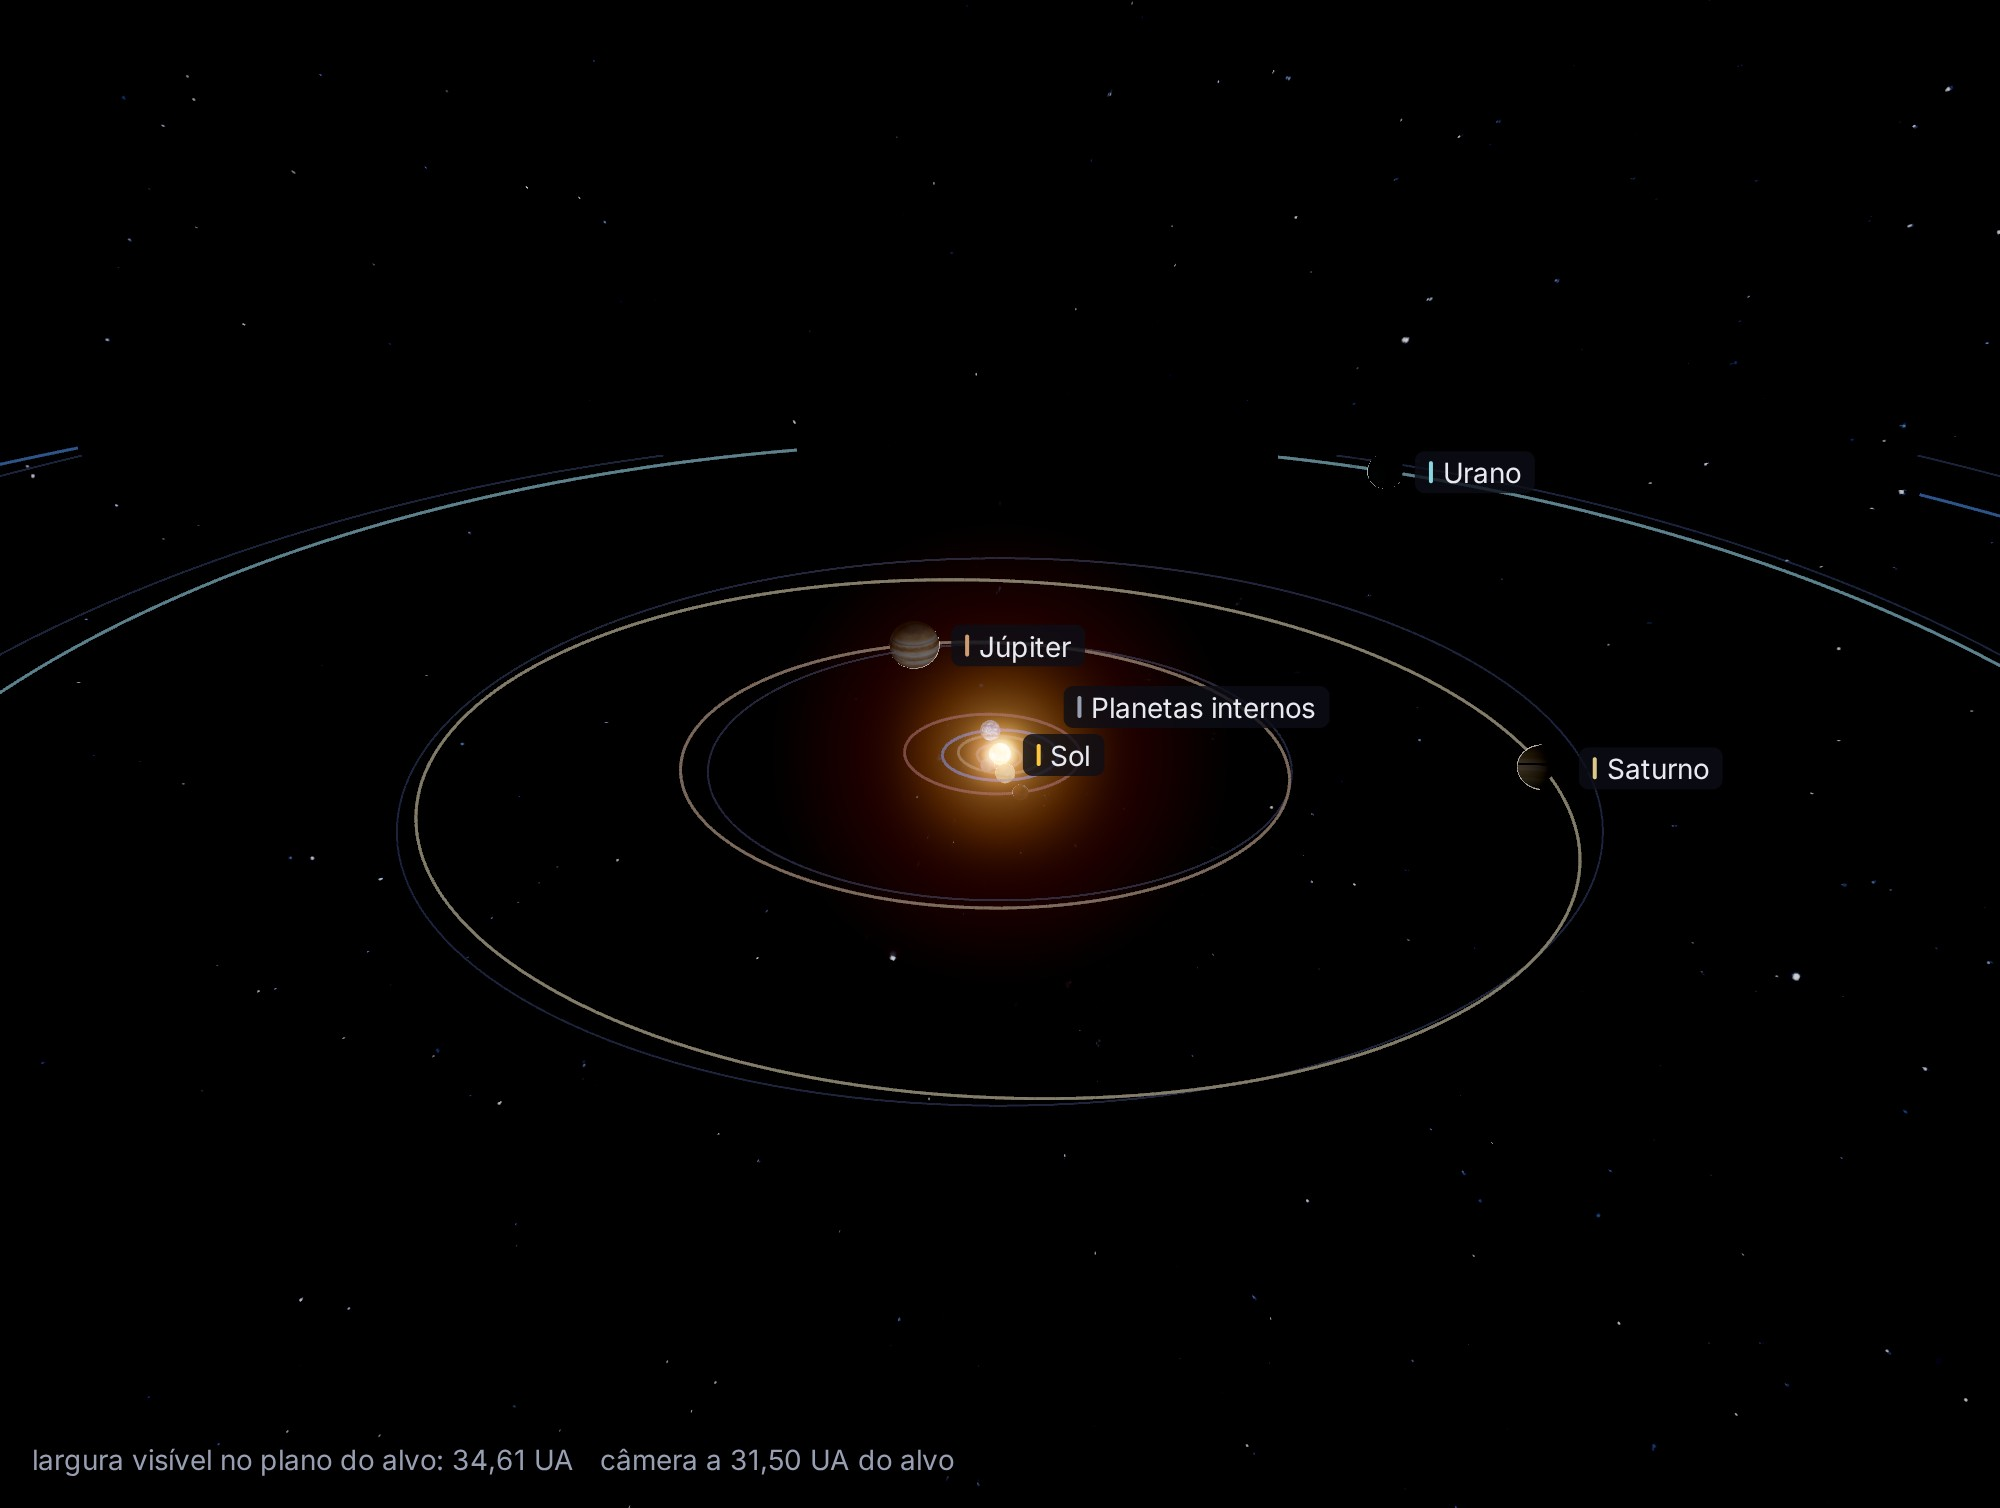
\includegraphics[width=\textwidth]{v3_visao_geral.jpg}
    \caption{Visão geral, a 31,5\,UA}
  \end{subfigure}\hfill
  \begin{subfigure}[b]{0.49\textwidth}
    \centering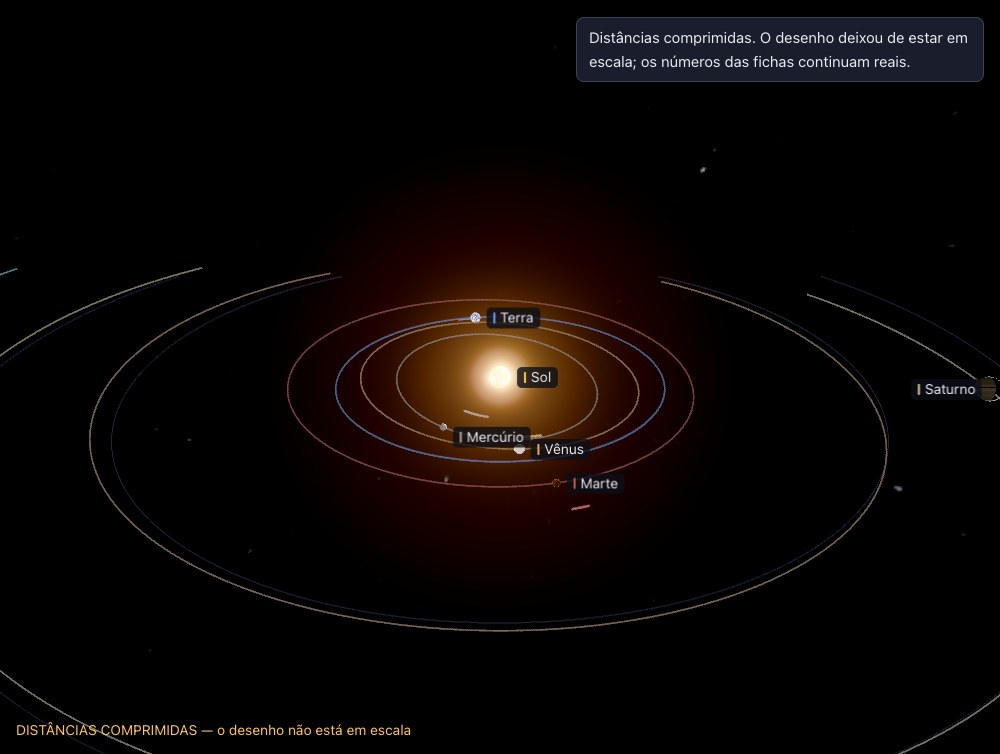
\includegraphics[width=\textwidth]{v3_maquete.jpg}
    \caption{Modo maquete, com o aviso}
  \end{subfigure}\\[4pt]
  \begin{subfigure}[b]{0.49\textwidth}
    \centering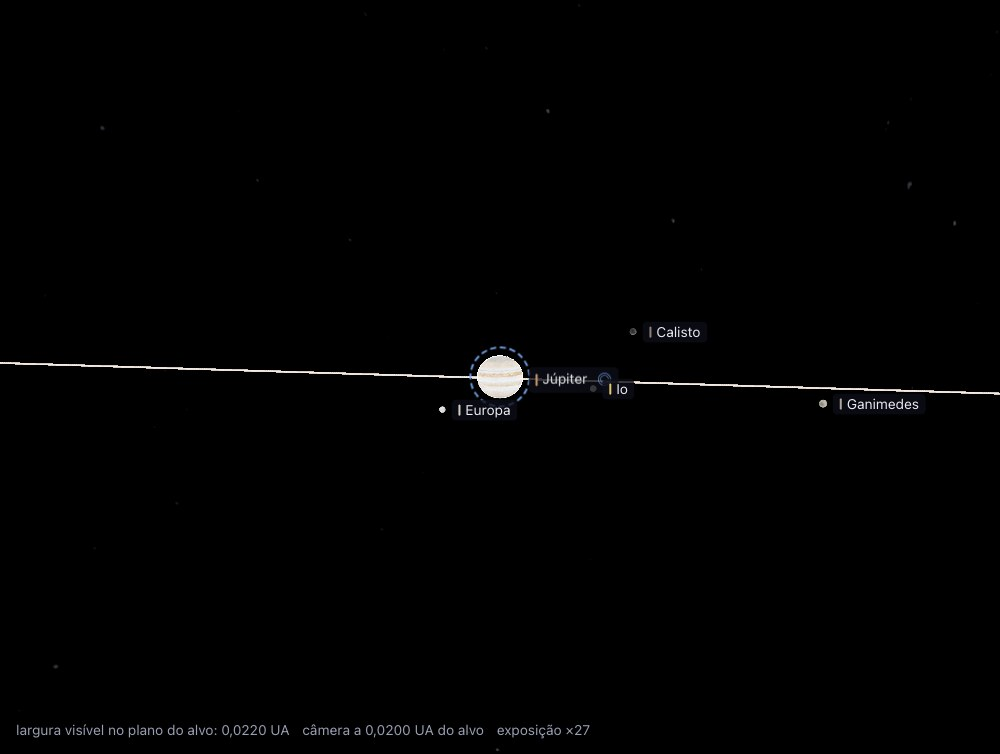
\includegraphics[width=\textwidth]{v3_jupiter_e_as_galileanas.jpg}
    \caption{Júpiter e as luas galileanas}
  \end{subfigure}\hfill
  \begin{subfigure}[b]{0.49\textwidth}
    \centering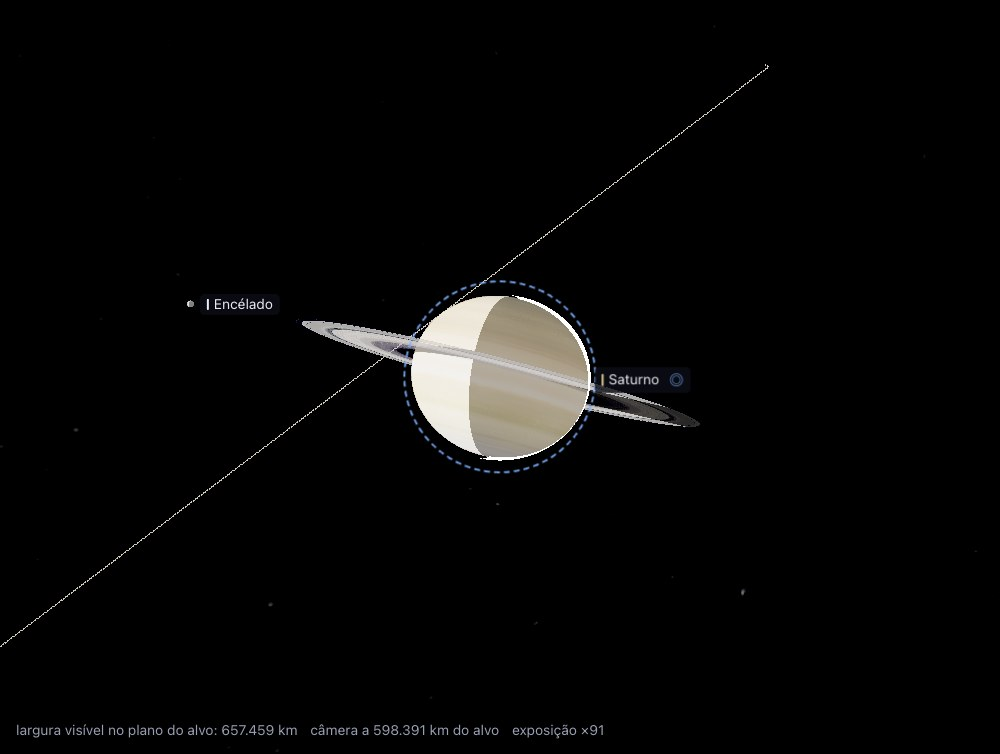
\includegraphics[width=\textwidth]{v3_saturno_e_os_aneis.jpg}
    \caption{Saturno, anéis e as duas sombras}
  \end{subfigure}\\[4pt]
  \begin{subfigure}[b]{0.49\textwidth}
    \centering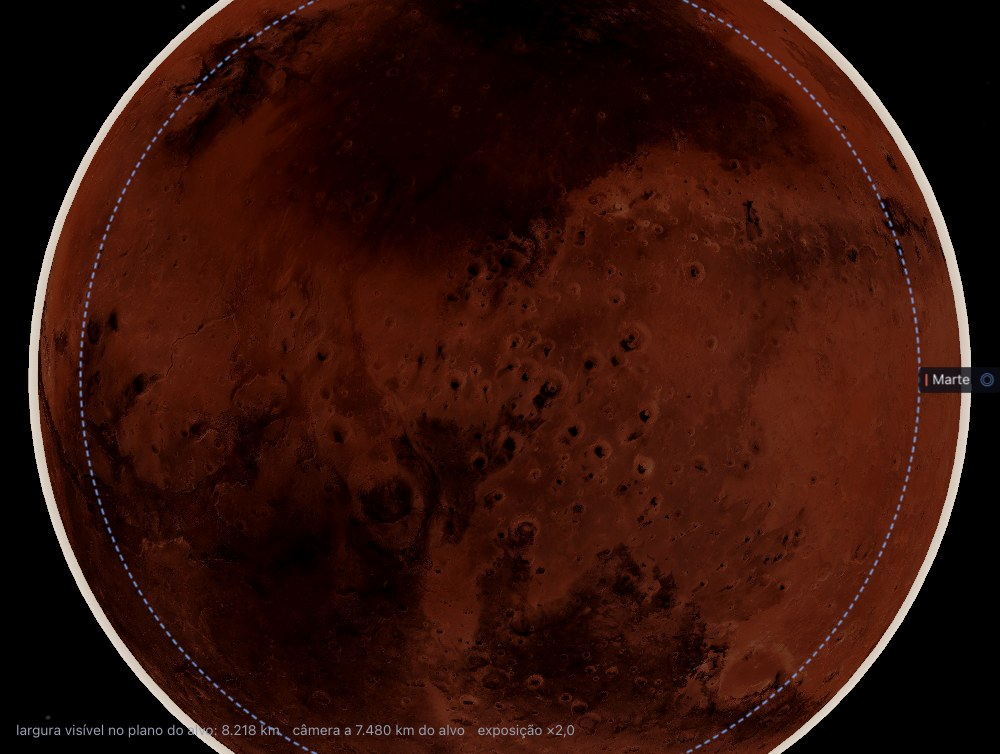
\includegraphics[width=\textwidth]{v3_marte_em_orbita_baixa.jpg}
    \caption{Marte a três raios, textura 8K}
  \end{subfigure}\hfill
  \begin{subfigure}[b]{0.49\textwidth}
    \centering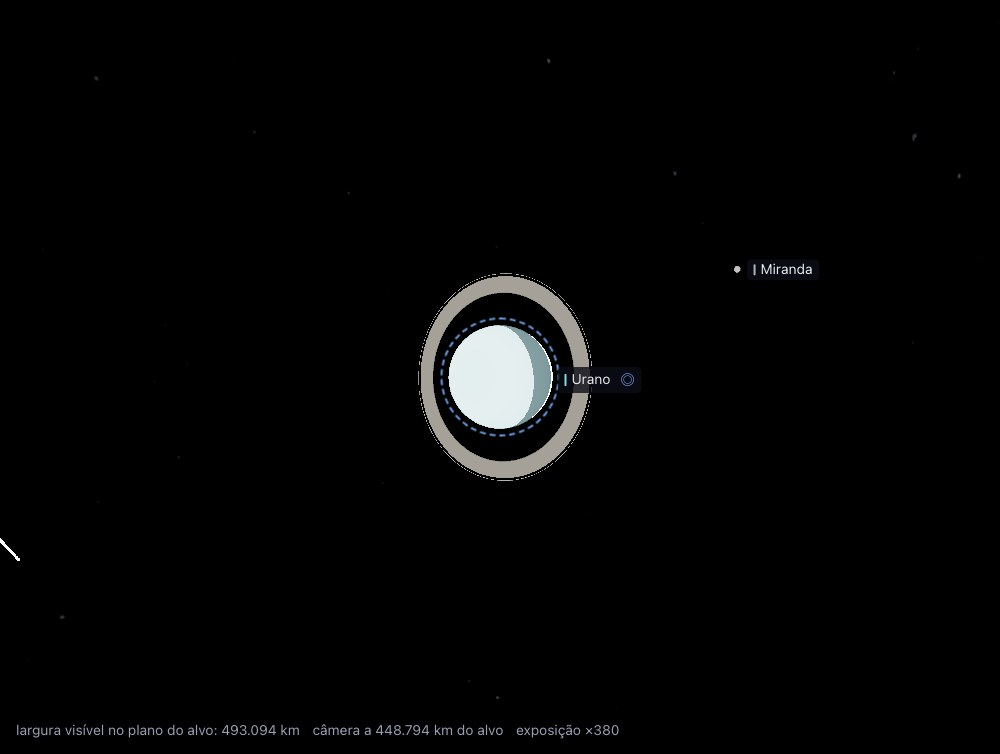
\includegraphics[width=\textwidth]{v3_urano_deitado.jpg}
    \caption{Urano, com eixo inclinado a $98^\circ$}
  \end{subfigure}
  \legend{Cenas de referência usadas pelos testes visuais automatizados. A barra inferior de cada cena traz a largura visível, a distância da câmera e o fator de exposição, escritos pelo próprio programa. Fonte: capturas do programa.}
\end{figure}

\paragraph{Arquitetura em camadas}

O código é dividido em camadas com regras de dependência verificadas automaticamente (\autoref{fig:camadas}). A regra central é que o núcleo físico não enxerga nada além de si mesmo: não sabe que existe uma tela, não lê o relógio do sistema, não sorteia números e não acessa a rede. Isso garante que a física possa ser testada sem navegador e que seja determinística. Sete regras, escritas num arquivo de configuração da ferramenta \emph{dependency-cruiser}, travam a compilação se alguém importar uma camada proibida. Uma regra de \emph{lint} proíbe ainda, dentro do núcleo, as quatro funções globais que quebrariam essas garantias em silêncio: \codigo{Math.random}, \codigo{Date.now}, \codigo{performance} e \codigo{fetch}.

\begin{figure}[htb]
  \centering
  \caption{Camadas da versão 3D e o sentido das dependências}
  \label{fig:camadas}
  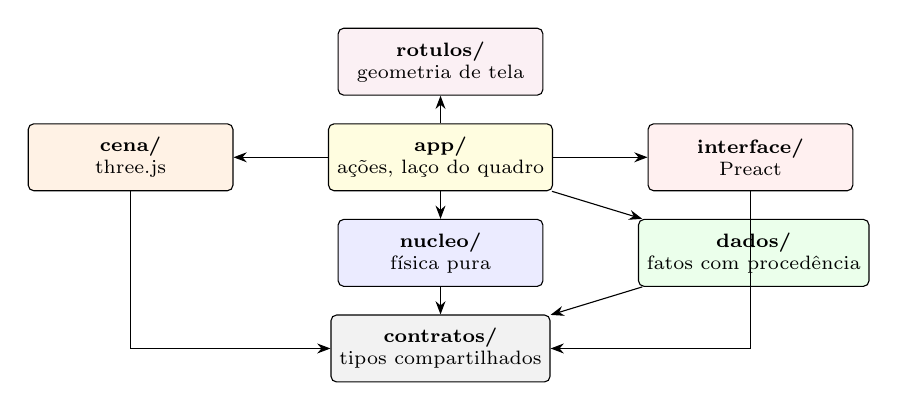
\begin{tikzpicture}[
      node distance=0.35cm and 0.6cm,
      cam/.style={draw,rounded corners=2pt,font=\scriptsize,align=center,minimum width=2.6cm,minimum height=0.85cm,inner sep=3pt},
      >=Stealth]
    \node[cam,fill=blue!8] (nucleo) {\textbf{nucleo/}\\física pura};
    \node[cam,fill=gray!10,below=of nucleo] (contratos) {\textbf{contratos/}\\tipos compartilhados};
    \node[cam,fill=green!8,right=1.2cm of nucleo] (dados) {\textbf{dados/}\\fatos com procedência};
    \node[cam,fill=yellow!12,above=of nucleo] (app) {\textbf{app/}\\ações, laço do quadro};
    \node[cam,fill=orange!10,left=1.2cm of app] (cena) {\textbf{cena/}\\three.js};
    \node[cam,fill=red!6,right=1.2cm of app] (interface) {\textbf{interface/}\\Preact};
    \node[cam,fill=purple!6,above=of app] (rotulos) {\textbf{rotulos/}\\geometria de tela};
    \draw[->] (app) -- (nucleo);
    \draw[->] (app) -- (dados);
    \draw[->] (app) -- (cena);
    \draw[->] (app) -- (interface);
    \draw[->] (app) -- (rotulos);
    \draw[->] (dados) -- (contratos);
    \draw[->] (nucleo) -- (contratos);
    \draw[->] (cena) |- (contratos);
    \draw[->] (interface) |- (contratos);
  \end{tikzpicture}
  \legend{Uma seta de A para B significa ``A pode importar B''. O núcleo e os dados não importam nenhuma camada de desenho; a cena não importa a aplicação, e por isso não consegue abrir uma janela nem disparar uma ação. Fonte: elaborada pelos autores a partir de \arquivo{ARQUITETURA.md}.}
\end{figure}

\paragraph{A origem flutuante}\label{sec:origem-flutuante}

Como discutido na \autoref{sec:float}, a placa gráfica trabalha em float32, e a subtração entre a posição da câmera e a de um corpo, ambas grandes, destrói a precisão. A solução adotada é a \emph{origem flutuante}: a câmera fica sempre na origem da cena, e a posição de cada corpo \emph{relativa à câmera} é calculada em float64, na CPU, antes de ir para a placa. A coluna de translação da matriz de vista é zero por construção. A alternativa ingênua, enviar as posições absolutas em float32, quantizaria a posição em cerca de 270\,km a 30\,UA e 13\,km a 1,5\,UA, e Fobos, com cerca de 11\,km de raio, ficaria do tamanho do quantum de posição do próprio planeta.

\paragraph{Fatias de profundidade}

Entre a superfície de um planeta vista de perto (cerca de 1\,km) e a órbita de Netuno ($4{,}5\times10^9$\,km) há nove ordens de grandeza. Um \emph{z-buffer} de 24 bits, que guarda a profundidade de cada pixel para decidir o que fica na frente, não distingue nada nessa faixa. O programa desenha a cena em \emph{fatias de profundidade}: a mais distante primeiro, depois limpa o z-buffer e desenha a mais próxima por cima, cada fatia com razão entre o plano distante e o próximo de no máximo $10^5$. A técnica não depende de recursos específicos do renderizador e funciona igualmente nos dois backends.

\paragraph{Luz, superfície e céu}

A iluminação tem uma única fonte, pontual, no Sol. A borda entre dia e noite, o \emph{terminador}, recebe uma penumbra da largura angular do disco solar visto do planeta,
\begin{equation}
  s = \frac{R_\odot}{d},\qquad
  \text{luz} = \operatorname{smoothstep}\bigl(-s,\,s,\,\hat{\vetor{n}}\cdot\hat{\vetor{l}}\bigr),
\end{equation}
em que $d$ é a distância real ao Sol, $\hat{\vetor{n}}$ a normal da superfície e $\hat{\vetor{l}}$ a direção do Sol. Sem ela o terminador vira uma linha dura que denuncia a computação gráfica. O lado noturno recebe um piso de 14\,\% da luz do meio-dia, um ajuste visual avisado na Ajuda: sem ele, Marte visto com o Sol atrás era um disco preto, e o programa existe para mostrar como os planetas são.

A orientação de cada corpo segue as constantes de rotação da IAU \cite{archinal2018}: polo norte em ascensão reta e declinação $(\alpha_0,\delta_0)$ e meridiano principal $W = W_0 + \dot W d$. Como a simulação roda na eclíptica, a matriz completa é $R_x(-\varepsilon_0)\,R_z(\alpha_0 + 90^\circ)\,R_x(90^\circ - \delta_0)\,R_z(W)$. As texturas de superfície vêm do Solar System Scope e, para cinco luas, dos mosaicos de imageamento real Voyager, Galileo e Cassini do USGS. O céu de fundo é o \emph{Yale Bright Star Catalogue} \cite{hoffleit1991}: 8\,404 estrelas na posição correta, com brilho dado pela magnitude, $L\propto 10^{-0{,}4(V-6{,}5)}$, e cor de corpo negro dada pela temperatura de cada uma.

\begin{licao}[: a esfera girada noventa graus]
O gerador de esferas do three.js constrói os polos sobre o eixo $y$, enquanto todo o resto do programa trata $z$ como polo. Durante várias fases, a textura de cada planeta esteve desenhada com o polo sobre o equador do corpo. Nenhum teste acusava: o teste de orientação media a \emph{matriz}, que sempre esteve certa, e as imagens de referência tinham sido gravadas já com o defeito, de modo que travavam o erro em vez de denunciá-lo. O defeito foi achado por uma pergunta que nenhum teste fazia, onde a textura cai na geometria, e passou a ter um teste com resposta conhecida: como a Lua tem rotação sincronizada, da Terra vê-se sempre a face com os grandes mares escuros. A área escura medida na imagem só sai certa se matriz, geometria, meridiano e mapa estiverem certos ao mesmo tempo.
\end{licao}

\paragraph{As luas}\label{sec:luas}

A versão 3D acrescenta treze luas: a Lua, Fobos, Deimos, as quatro galileanas, Encélado, Titã, Titânia, Oberon, Miranda e Tritão. Elas \emph{não} entram no integrador. Io dá uma volta em 1,77 dia; com passo de meio dia seriam três passos e meio por órbita, regime em que nenhum integrador de passo fixo funciona. Reduzir o passo global para atender a Io custaria o desempenho de todo o resto e alteraria a camada dinâmica validada contra o JPL.

As luas são propagadas analiticamente pela \autoref{sec:kepler}, a partir dos elementos médios publicados pelo JPL, com taxas seculares de precessão do nodo e do periastro:
\begin{equation}
  M(t) = M_0 + \dot M\,t,\qquad
  \Omega(t) = \Omega_0 + \dot\Omega\,t,\qquad
  \omega(t) = \omega_0 + \dot\omega\,t.
\end{equation}
Elas não puxam nada e não alteram o estado dos nove corpos. O preço é um erro limitado, medido numa janela de vinte anos que os dados de ajuste nunca viram (\autoref{sec:res-luas}). Ao gerar esses dados, apareceram três problemas que a página do JPL não menciona:

\begin{itemize}
  \item a coluna de período não é o período sideral de todas as luas. Em Io ela difere 0,36\,\% do período medido, o que em um ano desloca a lua 270 graus. O programa mede o período casando a fase entre duas janelas de vetores do Horizons separadas por dezesseis anos;
  \item cada lua usa um plano de referência: a eclíptica (só a Lua), o plano de Laplace (a maioria) ou o equador do planeta (as luas de Urano). Misturar os planos põe a lua no lugar errado sem nenhum erro visível;
  \item o polo de Urano: com o polo publicado pela IAU, Titânia, Oberon e Miranda saem retrógradas e erram 600 mil quilômetros. O gerador testa as duas orientações e grava a que reproduz as posições, com o erro de cada uma ao lado. O mesmo procedimento decidiu um fator $\cos i$ na relação entre as taxas, que só importa em Tritão, retrógrada: sem ele, o erro foi de 378 mil quilômetros, a lua do outro lado de Netuno.
\end{itemize}

\paragraph{O laboratório de Fourier complexo}

O laboratório da versão 3D implementa a série complexa (\autoref{alg:fourier}): a órbita osculadora do corpo selecionado é projetada no próprio plano, amostrada no tempo, decomposta uma única vez e desenhada como cadeia de epiciclos ordenada por raio decrescente. O termo $n=0$ é desenhado como um deslocamento fixo, e não como mais um círculo, porque desenhá-lo girando mostraria um movimento que não existe. A tela rotula a cadeia como ``construção histórica, não é a física do modelo'', para que ninguém saia achando que a simulação calcula epiciclos.

\begin{algorithm}[htb]
  \caption{Coeficientes de Fourier e cadeia de epiciclos}\label{alg:fourier}
  \KwIn{elementos $a$, $e$; número de amostras $A$; harmônicos $N$ com $2N < A$; instante $t\in[0,1)$}
  \KwOut{coeficientes $c_{-N..N}$ e os elos da cadeia no instante $t$}
  \For{$k\leftarrow 0$ \KwTo $A-1$}{
    $M \leftarrow 2\pi k/A$;\quad $E \leftarrow$ \textsc{ResolverKepler}$(M, e)$\;
    $z_k \leftarrow a(\cos E - e) + \ii\, a\sqrt{1-e^2}\sin E$\Com*[r]{amostra no tempo}
  }
  \For{$n\leftarrow -N$ \KwTo $N$}{
    $c_n \leftarrow \frac1A\sum_k z_k\,e^{-2\pi\ii nk/A}$\Com*[r]{\autoref{eq:dft}}
  }
  $p \leftarrow c_0$\Com*[r]{excêntrico: não gira}
  \ForEach{$n \neq 0$, em ordem decrescente de $|c_n|$}{
    $q \leftarrow p + c_n\,e^{2\pi\ii nt}$\;
    registrar elo (centro $p$, raio $|c_n|$, ponta $q$);\quad $p\leftarrow q$\;
  }
  \Return $c$, elos; a ponta $p$ é a posição reconstruída\;
\end{algorithm}

\paragraph{O modo de criação}

No \emph{sandbox}, a pessoa aponta um lugar da cena, escolhe um tipo de corpo (asteroide, cometa, planeta rochoso ou gasoso, estrela) e ajusta a velocidade num controle marcado de ``órbita redonda'' a ``escapa''. Antes de soltar, o programa mostra a órbita que o corpo teria. Duas guardas recusam, por escrito e com alternativa, criações que produziriam resultado numérico sem sentido: uma exige pelo menos 40 passos de integração por órbita, calculados no \emph{periélio} previsto e não na distância do clique, porque um corpo largado longe com velocidade quase radial passa raspando pelo Sol; a outra impede que o corpo nasça dentro da vizinhança gravitacional de outro. Quando a primeira recusa, o programa oferece um passo menor, de 0,125 dia, e o anuncia na tela enquanto ele estiver ligado. Todo sistema modificado exibe um distintivo permanente, ``não é mais a efeméride do JPL'', com o botão de voltar ao original.

\paragraph{Interface e acessibilidade}

A interface foi reorganizada \emph{por pergunta} e não por tipo de controle. A barra de cima responde a \emph{quando} (pausar, velocidade, data) e a \emph{o que estou fazendo} (explorar, criar, voar). O painel lateral responde a \emph{de onde vejo} e \emph{qual corpo}. Sobre a cena não há nenhum controle clicável. Todo o programa é operável por teclado, cada controle tem rótulo para leitores de tela, há uma opção que descreve a cena em forma de tabela, os contrastes de cor são medidos, e o modo de criação funciona sem arrastar, como pede o critério 2.5.7 das WCAG 2.2 \cite{wcag22}.

\subsection{Processo de desenvolvimento}\label{cap:processo}

Este capítulo descreve como o programa foi construído: o método de trabalho, os testes que sustentam as afirmações do texto e alguns erros encontrados pelo caminho. As instruções para instalar e executar o programa estão no fim do capítulo e, com mais detalhe, no \autoref{ap:execucao}.

\subsubsection{Princípio: toda afirmação tem um teste}

Desde a versão 2D, o documento de arquitetura estabelece que o que está escrito nele foi medido ou testado. Quando o programa afirma algo sobre si mesmo, na interface, na documentação ou num comentário de código, deve existir um teste automatizado que falhe se a afirmação deixar de valer.

A regra nasceu de três defeitos:

\begin{itemize}
  \item a documentação da versão 2D dizia que a física não dependia da camada de desenho, mas um módulo de interface importava um atalho da raiz do projeto. Hoje um teste lê a árvore sintática de cada arquivo e falha se a separação for quebrada;
  \item o ``modo maquete'' da versão 3D teve, durante uma fase inteira, o botão, o aviso falado e a etiqueta ``distâncias comprimidas'' na tela, e não comprimia nada;
  \item uma auditoria encontrou o contrato de funcionalidades citando catorze arquivos de teste que nunca existiram, em dezessete dos quarenta e três itens.
\end{itemize}

\subsubsection{O contrato de funcionalidades}\label{sec:contrato}

Antes de escrever o código da versão 3D, foi escrito um \emph{contrato}: a lista das 43 funcionalidades que a versão 2D entregava e que a 3D precisava entregar, agrupadas em tempo, câmera, cena, seleção, aprendizado e sistema. Sem ele, o risco era terminar com a física correta e os gráficos prontos, mas com parte do conteúdo educativo faltando, o que seria um retrocesso em relação ao programa que já funcionava.

Cada linha do contrato tem uma coluna \emph{prova}, com o teste automatizado que a verifica ou, em poucos casos, um roteiro manual de uma frase, e uma coluna \emph{estado}: pendente, feito, mudado (entrega o mesmo valor por outro meio, com justificativa) ou defeito. Nenhuma fase começava com uma linha vermelha na anterior. Ao final, 31 funcionalidades foram entregues como especificadas e 12 por outro meio, cada uma com uma nota. Um teste lê o contrato e exige que todo arquivo de prova citado exista e que a contagem do resumo bata com as linhas da tabela.

\subsubsection{Fases}

O desenvolvimento da versão 3D foi dividido em fases, cada uma com um critério de saída verificável:

\begin{description}
  \item[F0 -- Fundação.] Estrutura de pastas, regras de camada, servidor local, persistência de preferências.
  \item[F1 -- Física.] Porte do núcleo de Python para TypeScript, com os mesmos testes de conservação e reversibilidade.
  \item[F2 -- Interface acessível.] Controles por teclado e mouse, rótulos, avisos.
  \item[F3 -- Precisão do desenho.] Câmera, origem flutuante, fatias de profundidade, seleção em espaço de tela.
  \item[F4 -- Cena elaborada.] Texturas, iluminação, anéis, estrelas, rótulos.
  \item[F5 -- Conteúdo.] Fichas, ajuda, atividades, laboratório de Fourier.
  \item[F6 -- Luas.] Geração dos elementos, propagação e medida do erro.
  \item[F7 -- Sandbox.] Criação de corpos, guardas e desfazer.
  \item[F8 -- Entrega.] Empacotamento, cenas de referência, execução por duplo clique.
  \item[F9--F14 -- Refinamento.] Aproximação dos corpos, reorganização da interface, texturas 8K, desempenho e uma varredura sistemática de defeitos visuais.
\end{description}

Na última rodada, a busca de defeitos visuais foi feita em sete dimensões em paralelo, e cada achado foi depois atacado por um segundo revisor, encarregado de tentar refutá-lo lendo o código e os testes. Dos 40 achados, 35 resistiram à refutação.
% CONFERIR: o texto anterior dizia que os 35 "foram corrigidos". O tracker ACHADOS-VISUAIS.md marca só 7 como consertados.
% Atualizar esta frase quando o estado real for confirmado.

\subsubsection{Os testes}

O comando \codigo{npm test} roda cinco etapas em ordem, e qualquer falha interrompe as seguintes (\autoref{tab:portao}).

\begin{table}[htb]
  \centering
  \caption{O que cada etapa dos testes verifica}
  \label{tab:portao}
  \begin{tabularx}{\textwidth}{lX}
    \toprule
    Etapa & O que trava \\
    \midrule
    tipos & TypeScript em modo estrito, inclusive acesso a índice possivelmente inexistente \\
    lint & funções globais proibidas no núcleo; leitura de layout no caminho executado a cada quadro \\
    arquitetura & as sete regras de dependência entre camadas \\
    unidade & o núcleo físico em ambiente sem navegador (se a física tocar a página, quebra aqui); conservação, reversibilidade, validação contra o JPL, Kepler, Fourier, luas, sandbox; as guardas de texto \\
    ponta a ponta & o programa construído, num navegador sem janela: funcionamento sem internet, acessibilidade, teclado, conteúdo, contraste de rótulos medido no pixel, precisão de profundidade nos dois backends, laboratório, maquete, sandbox e doze cenas de referência \\
    \bottomrule
  \end{tabularx}
  \legend{A versão 3D tem 61 arquivos de teste, cerca de 10\,500 linhas e pouco mais de 500 casos. Fonte: elaborada pelos autores a partir de \arquivo{README.md}.}
\end{table}

Dois testes verificam texto, o que as ferramentas comuns não fazem. O \codigo{honestidade.test.ts} liga cada simplificação listada no bloco ``o que a tela simplifica'' a um fato do código, nos dois sentidos: listar uma simplificação que o código não faz reprova, e fazer uma que não está listada também. O \codigo{contrato.test.ts} faz o mesmo com o contrato de funcionalidades.

\begin{licao}[: um teste que mede o próprio teste]
Quatro testes passavam sem medir nada. Uma leitura de canvas feita fora do quadro devolvia um buffer vazio, e um buffer vazio é estável entre dois quadros, então o teste de tremulação passava com zero. Uma asserção algébrica era verdadeira para qualquer entrada. Um corpo de teste ``se movia'' com a gravidade desligada. Um teste de texto passou com o parágrafo apagado, porque as palavras apareciam em outro lugar da página. Desde então, toda medição vem com uma guarda que afirma que ela mede alguma coisa. Para conferir, basta sabotar o código e ver o teste ficar vermelho; se continuar verde, ele não mede o que diz.
\end{licao}

\subsubsection{Erros registrados}

O documento de arquitetura mantém uma tabela com os erros encontrados e a correção de cada um. A \autoref{tab:armadilhas} seleciona alguns, de classes diferentes.

\begin{table}[htb]
  \centering
  \caption{Alguns erros registrados durante o desenvolvimento}
  \label{tab:armadilhas}
  \small
  \begin{tabularx}{\textwidth}{>{\raggedright\arraybackslash}p{3.6cm}X}
    \toprule
    Erro & O que acontecia e o que se fez \\
    \midrule
    Ajustar e medir na mesma janela de dados &
    Mínimos quadrados forçam resíduo sem tendência \emph{dentro} da janela ajustada; medir ali mede o ajuste, não o modelo. As luas são ajustadas em 2000--2016 e conferidas em 2020--2040. \\
    Buscar corpo por índice numa lista que cresce &
    Depois de criar um corpo no sandbox, o índice de uma lua passou a apontar para o asteroide recém-criado, e a lua saía com o nome dele. Toda busca passou a ser por chave. \\
    $\mu = GM_i + GM_j$ numa guarda &
    Asteroides e cometas têm massa zero no programa; com a soma, dois deles poderiam nascer sobrepostos. A guarda passou a usar a $GM$ do vizinho. \\
    Abrir o programa por \codigo{file://} &
    O navegador bloqueia a leitura dos arquivos de dados por segurança. O programa sempre sobe um servidor local, que escuta só em \codigo{127.0.0.1}. \\
    Trava de servidor que sobrevive ao processo &
    Se o processo morria sem limpar a trava, o programa nunca mais abria e nada na tela dizia por quê. Agora a abertura verifica se o processo da trava ainda existe. \\
    Polo da IAU para Marte transcrito pela metade &
    A IAU publica o polo de Marte como constante mais um termo periódico de $1{,}59^\circ$, e só a constante fora copiada. Uma conferência cruzada entre o polo e a obliquidade de cada planeta achou o erro, e o de Netuno junto. \\
    \bottomrule
  \end{tabularx}
  \legend{Fonte: elaborada pelos autores a partir de \arquivo{ARQUITETURA.md} e \arquivo{CONTRATO.md}.}
\end{table}

\subsubsection{Ferramentas e uso de assistente de IA}

O desenvolvimento usou Python com NumPy \cite{harris2020} e Pygame nas duas primeiras versões, e TypeScript, Vite, three.js, Preact, Vitest e Playwright na terceira. Parte da programação, da revisão de código e da investigação de defeitos foi feita com o apoio do assistente Claude, da Anthropic \cite{anthropic2026}. Os resultados numéricos do \autoref{cap:resultados} podem ser reproduzidos pelos roteiros do \autoref{ap:experimentos}.
% CONFERIR: a frase anterior ("nenhuma afirmação entrou sem teste ou medição") não vale para os textos
% da interface. Ex.: a dica "Mercúrio está oito vezes mais perto do Sol que Júpiter" é falsa (são ~13 vezes).

\subsubsection{Como executar}

O programa é entregue como uma pasta. Na versão 3D, a pasta já traz o programa construído e os dados, e não exige instalação na máquina de quem recebe além do Node.js (ou, na falta dele, do Python, que serve como alternativa para o servidor local):

\begin{itemize}
  \item Windows: duplo clique em \arquivo{run.bat};
  \item macOS: duplo clique em \arquivo{run.command};
  \item Linux: \codigo{./run.sh}.
\end{itemize}

O lançador sobe um servidor local e abre o navegador. Fechar a aba encerra o programa. A versão 2D abre da mesma forma, com Python 3.9 ou superior, e prepara o ambiente sozinha na primeira execução. O \autoref{ap:execucao} traz o passo a passo, os comandos para desenvolvedores e a solução dos problemas mais comuns.

\section{Resultados}\label{cap:resultados}
% orçamento: 2.200 palavras

Este capítulo reúne os resultados quantitativos. Os números das \autoref{sec:res-validacao} e \ref{sec:res-integradores} foram obtidos por uma segunda implementação do núcleo físico, em Python e NumPy, escrita para este relatório a partir do mesmo arquivo de condições iniciais. Ela reproduz, até a última casa decimal publicada, a tabela de validação da documentação do programa. Como usa o mesmo algoritmo e o mesmo passo, confirma o porte para TypeScript, não a física; a física é validada pela comparação com o JPL. Os roteiros estão no \autoref{ap:experimentos}.

\subsection{Validação contra a efeméride do JPL}\label{sec:res-validacao}

Partindo de 1º de janeiro de 2026, o sistema de nove corpos foi integrado para a frente e para trás e comparado com as posições do JPL Horizons nas mesmas datas. O critério de aceitação, fixado \emph{antes} de olhar os resultados, foi erro inferior a 1\,\% da distância ao Sol para todos os corpos no intervalo de $-100$ a $+100$ anos. A comparação foi feita em cinco datas ($-100$, $-10$, $+1$, $+10$ e $+100$ anos), não em varredura contínua. A \autoref{tab:validacao} e a \autoref{fig:validacao} mostram o resultado.

\begin{table}[htb]
  \centering
  \caption{Erro de posição contra o JPL Horizons, em quilômetros}
  \label{tab:validacao}
  \small
  \setlength{\tabcolsep}{4pt}
  \begin{tabular}{lrrrrrrrrr}
    \toprule
    Intervalo & Sol & Mercúrio & Vênus & Terra & Marte & Júpiter & Saturno & Urano & Netuno \\
    \midrule
    $-100$ anos & 153 & 247\,115 & 5\,612 & 4\,782 & 3\,420 & 195 & 173 & 238 & 709 \\
    $-10$ anos  & 4   & 15\,637  & 556    & 489    & 297    & 35  & 8   & 3   & 7 \\
    $+1$ ano    & 0,2 & 3\,048   & 61     & 49     & 35     & 0,4 & 0,1 & 0,0 & 0,1 \\
    $+10$ anos  & 1   & 14\,365  & 534    & 487    & 368    & 41  & 5   & 3   & 7 \\
    $+100$ anos & 112 & 302\,436 & 5\,725 & 4\,763 & 4\,180 & 164 & 142 & 210 & 636 \\
    \bottomrule
  \end{tabular}
  \legend{Integrador de Yoshida de quarta ordem, passo de 0,5 dia, posições relativas ao baricentro do Sistema Solar. Fonte: elaborada pelos autores.}
\end{table}

\begin{figure}[htb]
  \centering
  \caption{Erro relativo à distância ao Sol}
  \label{fig:validacao}
  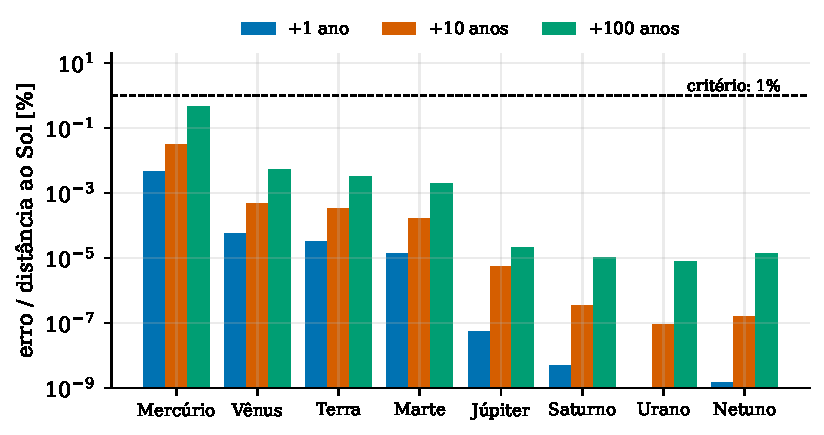
\includegraphics[width=0.95\textwidth]{validacao.pdf}
  \legend{Escala logarítmica. A linha tracejada é o critério de 1\,\%. Fonte: elaborada pelos autores.}
\end{figure}

Todos os corpos passam com folga. O pior caso é Mercúrio: 0,004\,\% da distância ao Sol em um ano, 0,03\,\% em dez e 0,45\,\% em cem. Mercúrio é o caso difícil por duas razões. É o planeta mais rápido, com apenas 176 passos de integração por órbita, e por isso o erro de truncamento do passo pesa mais nele. E é o mais afetado pela relatividade geral, que o modelo não inclui (\autoref{sec:nao-inclui}). Em cem anos, a conservação ficou em $2\times10^{-9}$ para a energia relativa e $1{,}4\times10^{-14}$ para o momento angular.

\subsection{Escolha do integrador}\label{sec:res-integradores}

\subsubsection{Custo e precisão}

A \autoref{fig:trabalho-precisao} compara três integradores pelo critério que importa num programa interativo: quanta precisão se obtém por unidade de custo. O custo é contado em avaliações da força (o \autoref{alg:forca}), que dominam o tempo de execução. A precisão é o erro de Mercúrio após dez anos.

\begin{figure}[htb]
  \centering
  \caption{Precisão em função do custo para três integradores}
  \label{fig:trabalho-precisao}
  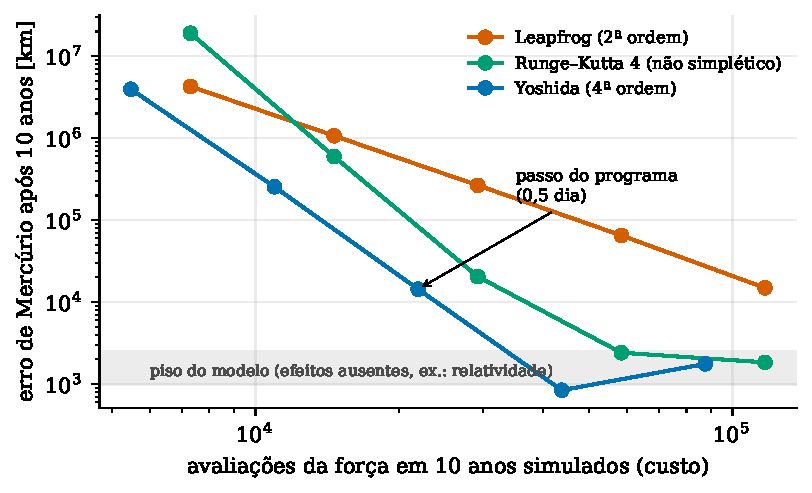
\includegraphics[width=0.9\textwidth]{trabalho_precisao.pdf}
  \legend{Cada ponto é um tamanho de passo. Leapfrog: de 0,5 a 1/32 dia; Yoshida e RK4: de 2 a 0,125 dia. A faixa cinza marca o patamar abaixo do qual o erro não cai, por menor que seja o passo. Fonte: elaborada pelos autores.}
\end{figure}

Do gráfico saem três leituras:

\begin{enumerate}
  \item As inclinações das curvas confirmam as ordens teóricas: reduzir o passo à metade divide o erro do leapfrog por cerca de 4 ($\Delta t^2$) e o do Yoshida por cerca de 16 ($\Delta t^4$), enquanto o passo é grande o bastante para que o truncamento domine.
  \item No passo escolhido, 0,5 dia, o Yoshida gasta 21\,912 avaliações e erra $1{,}4\times10^4$\,km. O leapfrog precisa de mais de 116\,000 avaliações, mais de cinco vezes o custo, para chegar ao mesmo erro.
  \item Abaixo de cerca de $10^3$\,km o erro deixa de cair. Esse patamar não vem do integrador, mas do \emph{modelo}: do que a integração não inclui. Sua ordem de grandeza coincide com a estimativa do efeito relativístico sobre Mercúrio em dez anos feita na \autoref{sec:nao-inclui}. Diminuir o passo além desse ponto só gasta tempo.
\end{enumerate}

\subsubsection{Conservação de energia a longo prazo}

A \autoref{fig:energia} integra o sistema por mil anos com passo deliberadamente grande, de 2 dias, para tornar visível o comportamento qualitativo. O RK4, que não é simplético, apresenta deriva sistemática: ao fim, a energia relativa mudou $4\times10^{-4}$, e a tendência continua. Os dois métodos simpléticos oscilam numa faixa fixa, de $10^{-5}$ para o leapfrog e $3\times10^{-7}$ para o Yoshida, sem tendência. Essa propriedade pesou mais na escolha que a precisão de um passo isolado: um programa que pode ficar rodando por séculos simulados não pode ter órbitas que encolhem ou se expandem aos poucos.

\begin{figure}[htb]
  \centering
  \caption{Erro relativo de energia em mil anos, com passo de 2 dias}
  \label{fig:energia}
  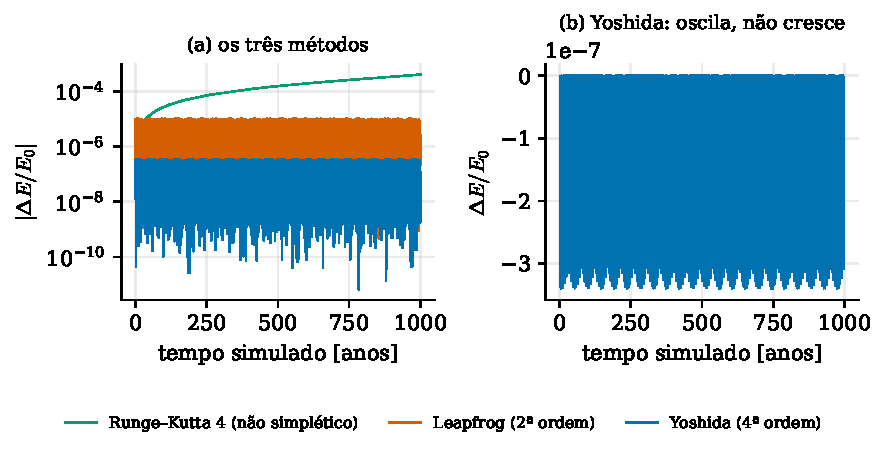
\includegraphics[width=\textwidth]{energia.pdf}
  \legend{(a) Valor absoluto do erro, em escala logarítmica: o RK4 cresce, os simpléticos não. (b) O erro do Yoshida em escala linear: uma oscilação rápida dentro de uma faixa fixa. Fonte: elaborada pelos autores.}
\end{figure}

\begin{noprograma}
Em ``Mostrar dados técnicos'', o programa exibe ao vivo o desvio de energia e de momento angular desde o início da simulação. Deixando o tempo correr por séculos, vê-se o número oscilar sem crescer, o que mostra na prática o significado da palavra simplético.
\end{noprograma}

\subsection{Séries de Fourier das órbitas}\label{sec:res-fourier}

\subsubsection{Convergência}

A \autoref{tab:fourier} e a \autoref{fig:convergencia} mostram, para a elipse osculadora de cada planeta em 1/1/2026, o desvio médio entre a série truncada em $|n|\leq N$ e a órbita. O número de harmônicos necessário cresce com a excentricidade: Vênus, quase circular, chega ao piso de arredondamento ($10^{-12}$\,UA, cerca de 15\,cm) com 6 harmônicos; Mercúrio precisa de 18.

\begin{table}[htb]
  \centering
  \caption{Desvio médio da série truncada em relação à órbita de Kepler}
  \label{tab:fourier}
  \small
  \begin{tabular}{lcrrrc}
    \toprule
    Planeta & $e$ & $|n|\leq1$ (km) & $|n|\leq2$ (km) & $|n|\leq3$ (km) & $N$ até $10^{-12}$\,UA \\
    \midrule
    Mercúrio & 0,2056 & 5\,800\,825  & 887\,349   & 160\,766 & 18 \\
    Vênus    & 0,0068 & 366\,870    & 1\,866     & 11       & 6 \\
    Terra    & 0,0167 & 1\,246\,726 & 15\,587    & 231      & 7 \\
    Marte    & 0,0935 & 10\,597\,766 & 741\,792  & 61\,528  & 12 \\
    Júpiter  & 0,0483 & 18\,756\,268 & 678\,692  & 29\,105  & 10 \\
    Saturno  & 0,0554 & 39\,450\,189 & 1\,636\,812 & 80\,485 & 11 \\
    Urano    & 0,0468 & 67\,447\,711 & 2\,367\,664 & 98\,502 & 10 \\
    Netuno   & 0,0111 & 25\,028\,289 & 208\,577  & 2\,060   & 7 \\
    \bottomrule
  \end{tabular}
  \legend{Elementos osculadores heliocêntricos em 1/1/2026, 720 amostras no tempo. Com $|n|\leq1$ a série tem três termos ($c_{-1}$, $c_0$, $c_1$); falta o epiciclo $c_2\approx\frac12 ae$, que domina o desvio. Fonte: elaborada pelos autores.}
\end{table}

\begin{figure}[htb]
  \centering
  \caption{Convergência da série de Fourier}
  \label{fig:convergencia}
  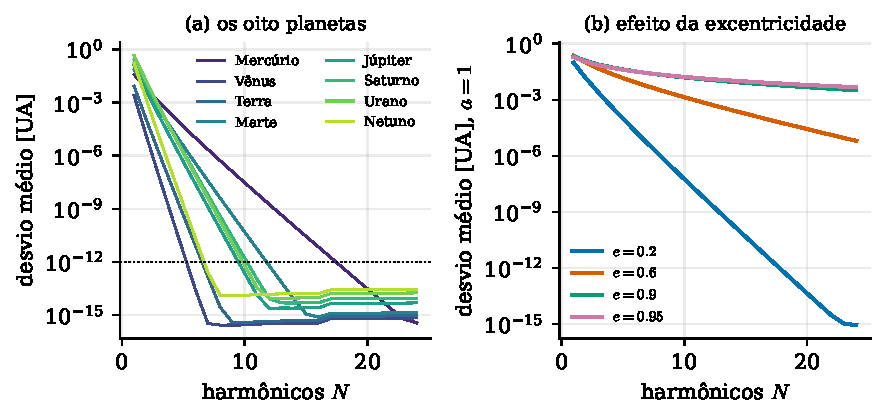
\includegraphics[width=\textwidth]{convergencia.pdf}
  \legend{(a) Os oito planetas; a linha pontilhada é o piso de $10^{-12}$\,UA. (b) Órbitas hipotéticas com $a = 1$\,UA: quanto mais alongada, mais devagar a série converge. Fonte: elaborada pelos autores.}
\end{figure}

Em termos absolutos os desvios com poucos termos são grandes: milhões de quilômetros para os planetas externos com $|n|\leq1$. Em termos relativos, porém, com $|n|\leq1$ o desvio de Júpiter já é de 2,4\,\% do semieixo, e com $|n|\leq2$ todos os planetas, exceto Mercúrio, ficam abaixo de 0,4\,\% (Júpiter, 0,09\,\%). É o que \citeonline{farias2016} observou nos gráficos: dois ou três termos já são uma excelente aproximação, com a exceção de Mercúrio.

\subsubsection{Conferência da forma fechada}

Os coeficientes calculados numericamente pela \autoref{eq:dft} foram comparados com a forma fechada da \autoref{eq:cn-bessel}. Para Mercúrio, com $|n|\leq 24$, a maior diferença foi de $2\times10^{-16}$\,UA, o arredondamento da aritmética de dupla precisão. Para órbitas hipotéticas com $a = 1$\,UA, a diferença foi de $4\times10^{-16}$ em $e = 0{,}6$, $1{,}2\times10^{-14}$ em $e = 0{,}9$ e $1{,}4\times10^{-8}$ em $e=0{,}95$. Neste último caso o aliasing descrito na \autoref{sec:dft} já aparece: o espectro decai devagar demais para 720 amostras. A relação $c_0 = -\frac32 ae$ (\autoref{eq:c0}) se verificou com erro relativo de $10^{-15}$ para os oito planetas.

\subsection{Copérnico revisitado}\label{sec:copernico-revisitado}

O \autoref{sec:pequeno-e} mostrou que, até primeira ordem na excentricidade, a série de Fourier no tempo de uma órbita kepleriana tem três termos: um deslocamento fixo $c_0 = -\frac32 ae$, um deferente $c_1\approx a$ e um epiciclo $c_2\approx\frac12 ae$ que gira com o dobro da frequência (\autoref{eq:copernico-fourier}).

Considere agora o modelo do \emph{Commentariolus} (\autoref{tab:copernico-raios}). Na descrição usual do mecanismo \cite{gallavotti1999,sugon2008}, o centro do primeiro epiciclo percorre o deferente, centrado no centro da órbita da Terra (o Sol médio, deslocado do Sol), enquanto o raio do epiciclo gira em sentido contrário com o mesmo período, de modo que, \emph{visto de fora}, ele mantém orientação fixa. O segundo epiciclo, montado na ponta do primeiro, gira duas vezes por período. Escrevendo cada movimento como número complexo, com a anomalia média $M$ medida a partir do periélio,
\begin{equation}
  z_\text{Copérnico}(M) = -r_1 + R\,e^{\ii M} + r_2\,e^{2\ii M}.
  \label{eq:copernico-modelo} % PENDENTE-E5: efeito do Sol médio em c0 (Tarefa 10)
\end{equation}
É a \autoref{eq:copernico-fourier} com $R \leftrightarrow a$, $r_1 \leftrightarrow \frac32 ae$ e $r_2 \leftrightarrow \frac12 ae$. Em particular, o modelo de Copérnico tem $r_1/r_2 = 3$ para \emph{todos} os planetas, e essa é exatamente a razão $\frac32 : \frac12$ que a série de Fourier impõe. A \autoref{tab:copernico-fourier} e a \autoref{fig:copernico} comparam os números.

\begin{table}[htb]
  \centering
  \caption{Raios de Copérnico comparados com os coeficientes de Fourier da órbita moderna}
  \label{tab:copernico-fourier}
  \small
  \setlength{\tabcolsep}{4.5pt}
  \begin{tabular}{l cc cc cc cc}
    \toprule
    & \multicolumn{2}{c}{Deferente} & \multicolumn{2}{c}{Excêntrico} & \multicolumn{2}{c}{Epiciclo duplo} & \multicolumn{2}{c}{Excentricidade} \\
    \cmidrule(lr){2-3}\cmidrule(lr){4-5}\cmidrule(lr){6-7}\cmidrule(lr){8-9}
    Planeta & $R$ & $a$ & $r_1$ & $|c_0|$ & $r_2$ & $|c_2|$ & $\frac{r_1}{1{,}5R}$ & $e$ \\
    \midrule
    Mercúrio & 0,376 & 0,387 & 0,067 & 0,119 & 0,023 & 0,039 & 0,119 & 0,206 \\
    Vênus    & 0,720 & 0,723 & 0,030 & 0,007 & 0,010 & 0,002 & 0,028 & 0,007 \\
    Marte    & 1,520 & 1,524 & 0,223 & 0,214 & 0,074 & 0,071 & 0,098 & 0,093 \\
    Júpiter  & 5,217 & 5,202 & 0,404 & 0,377 & 0,135 & 0,125 & 0,052 & 0,048 \\
    Saturno  & 9,207 & 9,546 & 0,787 & 0,793 & 0,263 & 0,264 & 0,057 & 0,055 \\
    \bottomrule
  \end{tabular}
  \legend{Raios em unidades astronômicas, convertidos das partes de Copérnico dividindo por 25. Os coeficientes $|c_0|$ e $|c_2|$ são da órbita osculadora em 1/1/2026. Fonte: elaborada pelos autores, com os raios de Copérnico de \citeonline{farias2016}.}
\end{table}

\begin{figure}[htb]
  \centering
  \caption{Os epiciclos de Copérnico e os coeficientes de Fourier}
  \label{fig:copernico}
  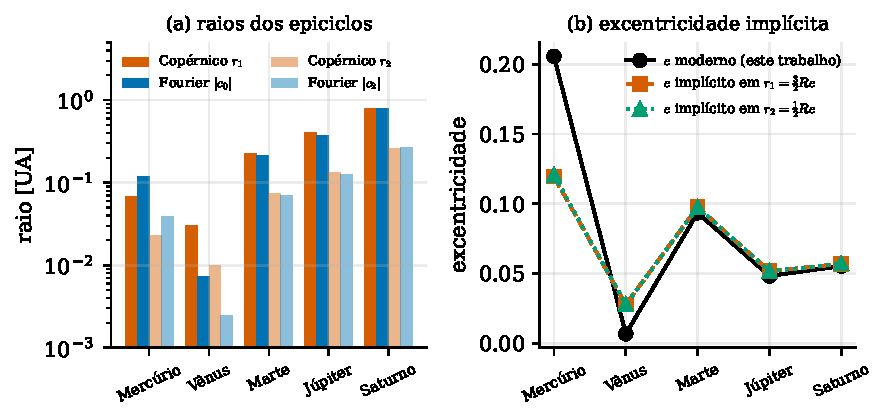
\includegraphics[width=\textwidth]{copernico.pdf}
  \legend{(a) Raios em escala logarítmica. (b) A excentricidade implícita em cada epiciclo de Copérnico, comparada com a moderna; as duas estimativas coincidem porque $r_1/r_2 = 3$. Fonte: elaborada pelos autores.}
\end{figure}

Para Marte, Júpiter e Saturno a concordância é boa. Os deferentes reproduzem os semieixos com erro de 0,2\,\% a 3,6\,\%, e os dois epiciclos reproduzem $|c_0|$ e $|c_2|$ com erro de 0,4\,\% a 8\,\%. A excentricidade implícita nos raios de Copérnico, $r_1/(1{,}5R)$, fica a menos de 0,005 da moderna nos três casos. Com a mesma métrica usada na \autoref{sec:res-fourier}, o modelo de Copérnico com os números dele erra a posição de Marte em no máximo 0,017\,UA, ou 1,1\,\% do semieixo; o de Júpiter em 0,9\,\%. Em Saturno o erro chega a 3,6\,\%, quase todo vindo do deferente, e não dos epiciclos.

Para Mercúrio e Vênus a concordância é pior, e por razões diferentes. Em Mercúrio a excentricidade é grande o bastante para que os termos de segunda ordem, desprezados na \autoref{eq:copernico-fourier}, cheguem a 10--15\,\% dos de primeira; além disso, o modelo de Mercúrio é historicamente o mais complicado da astronomia pré-kepleriana. Em Vênus a órbita é quase circular, e a excentricidade implícita (0,028) é quatro vezes a real; uma hipótese plausível, que não investigamos, é que os dados de Copérnico para Vênus carreguem a marca da excentricidade da própria órbita da Terra (0,017), da qual um planeta interior é sempre observado.

\begin{paraaprofundar}[: a relação com o TCC]
\citeonline{farias2016} comparou os raios de Copérnico com os raios da série de Fourier das órbitas reais e concluiu que eles têm a mesma ordem de grandeza, especialmente o primeiro epiciclo. Nas simulações daquele trabalho, o primeiro epiciclo foi modelado girando com frequência $-\omega$ e o segundo com $2\omega$, e uma modificação para as frequências $\omega$, $2\omega$ e $3\omega$ melhorou o ajuste. A leitura adotada aqui atribui ao primeiro epiciclo frequência \emph{zero} no referencial fixo, o que transforma o primeiro epiciclo no excêntrico $c_0$. Com essa atribuição, a comparação passa a ser termo a termo e a concordância passa de ordem de grandeza para poucos por cento. Com a mesma métrica, o modelo com frequências $(1, -1, 2)$ erra a posição de Marte em até 0,44\,UA, contra 0,017\,UA da leitura com frequência zero. O resultado não seria possível sem a organização dos dados históricos feita naquele trabalho. A conclusão de \citeonline{farias2016} de que um modelo ``heliostático'', com o Sol fora do centro do deferente, seria mais preciso é, nessa leitura, exatamente o que Copérnico fez: o excêntrico $r_1$ é o deslocamento entre o Sol e o centro efetivo do movimento.
\end{paraaprofundar}

Em primeira ordem na excentricidade, portanto, os raios do modelo de Copérnico para Marte, Júpiter e Saturno reproduzem os coeficientes da série de Fourier da órbita kepleriana, e a razão entre os dois epiciclos é a da série. Não comparamos esse resultado com outros modelos da mesma ordem, como o de Ptolomeu com equante. Sem essa comparação, os números mostram que os raios de Copérnico estavam bem estimados, mas não que o modelo dele seja o único a reproduzir a série.

\subsection{Solução da equação de Kepler}

A \autoref{fig:kepler-iteracoes} mede o número de iterações de Newton necessário para resolver a \autoref{eq:kepler} com tolerância de $10^{-13}$, no pior valor de $M$, para cada excentricidade. Com o chute $E_0 = M$, a convergência é rápida até $e\approx 0{,}98$, mas a partir daí há valores de $M$, perto do periélio, em que o método oscila e não converge. Com o chute de Danby, nunca são necessárias mais de 12 iterações, mesmo em $e = 0{,}999$. Os planetas, com $e < 0{,}21$, nunca precisam de mais de 5. O teste mostra também que o limite de 0,8 citado num comentário do código para a falha do chute $E_0=M$ é conservador; o limite medido é perto de 0,99.

\begin{figure}[htb]
  \centering
  \caption{Iterações de Newton para resolver a equação de Kepler}
  \label{fig:kepler-iteracoes}
  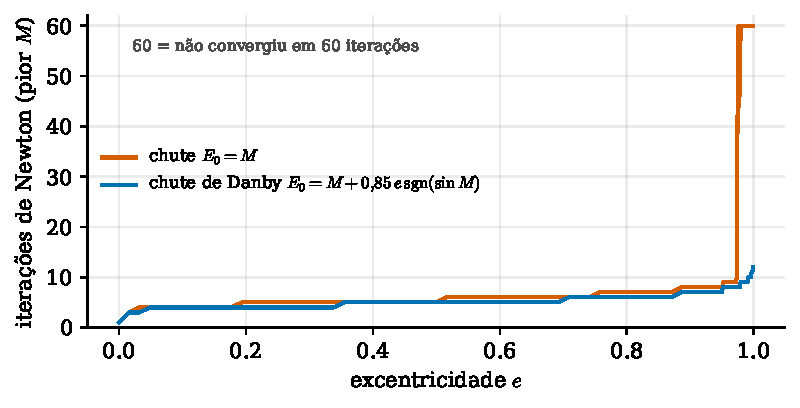
\includegraphics[width=0.85\textwidth]{kepler_iteracoes.pdf}
  \legend{Pior caso sobre $M\in(0,2\pi)$, com amostragem refinada perto de $M = 0$. Fonte: elaborada pelos autores.}
\end{figure}

\subsection{Erro das luas}\label{sec:res-luas}

A \autoref{tab:luas} mostra o erro de posição das treze luas propagadas analiticamente, medido contra o JPL Horizons entre 2020 e 2040, a cada 13 dias. Os parâmetros foram ajustados em dados de 2000 a 2016, de modo que essa janela mede o erro do \emph{modelo} e não o do ajuste. O erro não cresce de forma sistemática: a razão entre o pior erro da segunda e o da primeira metade da janela fica entre 0,97 e 1,07 para seis das treze luas e não passa de 1,7 em nenhuma. Ele vem de termos periódicos, como as ressonâncias entre as galileanas, que um modelo de dois corpos com precessão não contém.

\begin{table}[htb]
  \centering
  \caption{Erro das luas contra o JPL Horizons, 2020--2040}
  \label{tab:luas}
  \small
  \begin{tabular}{llrrrr}
    \toprule
    Lua & Planeta & $a$ (km) & Erro máximo (km) & Erro RMS (km) & Máximo / $a$ \\
    \midrule
    Lua      & Terra   & 384\,400   & 15\,293 & 7\,655  & 4,0\,\% \\
    Fobos    & Marte   & 9\,375     & 822     & 375     & 8,8\,\% \\
    Deimos   & Marte   & 23\,457    & 456     & 279     & 1,9\,\% \\
    Io       & Júpiter & 421\,800   & 7\,699  & 3\,943  & 1,8\,\% \\
    Europa   & Júpiter & 671\,100   & 25\,702 & 13\,725 & 3,8\,\% \\
    Ganimedes& Júpiter & 1\,070\,400 & 4\,295 & 2\,265  & 0,4\,\% \\
    Calisto  & Júpiter & 1\,882\,700 & 3\,587 & 2\,546  & 0,2\,\% \\
    Encélado & Saturno & 238\,400   & 5\,710  & 2\,679  & 2,4\,\% \\
    Titã     & Saturno & 1\,221\,900 & 37\,329 & 21\,211 & 3,1\,\% \\
    Titânia  & Urano   & 436\,298   & 2\,088  & 977     & 0,5\,\% \\
    Oberon   & Urano   & 583\,511   & 2\,476  & 1\,372  & 0,4\,\% \\
    Miranda  & Urano   & 129\,846   & 9\,423  & 5\,789  & 7,3\,\% \\
    Tritão   & Netuno  & 354\,800   & 52\,636 & 29\,194 & 14,8\,\% \\
    \bottomrule
  \end{tabular}
  \legend{Fonte: arquivo \arquivo{derivaDasLuas.json}, gerado por \arquivo{ferramentas/conferir\_luas.mjs}.}
\end{table}

\subsection{Fenômenos que emergem da simulação}

Nada no código manda o Sol se mover nem Marte recuar no céu. Os dois movimentos resultam da integração, o que os torna bons exemplos para a sala de aula.

O primeiro é o movimento retrógrado de Marte, já mostrado na \autoref{fig:marte-retrogrado}: o programa prevê a retrogradação de 2027 entre 10 de janeiro e 1º de abril. O segundo é o movimento do Sol em torno do centro de massa do sistema (\autoref{fig:sol-baricentro}). Em cinquenta anos, o centro do Sol percorre um emaranhado de laços que chega a 1,8 raio solar do baricentro: o centro de massa do Sistema Solar fica, boa parte do tempo, \emph{fora} do Sol. O padrão é dominado por Júpiter, com período de 12 anos, modulado por Saturno. É esse movimento que, medido em outras estrelas pelo efeito Doppler, revela a existência de planetas extrassolares.

\begin{figure}[htb]
  \centering
  \caption{O centro do Sol em torno do centro de massa do sistema, 2026--2076}
  \label{fig:sol-baricentro}
  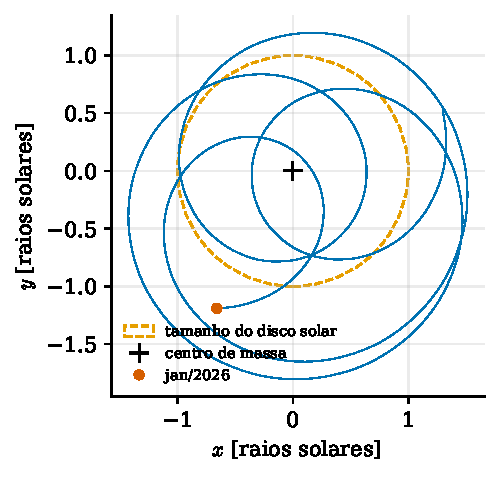
\includegraphics[width=0.55\textwidth]{sol_baricentro.pdf}
  \legend{Projeção no plano da eclíptica. O círculo tracejado tem o raio do Sol. Fonte: elaborada pelos autores com o integrador do programa.}
\end{figure}

\section{Discussão, limitações e uso em sala de aula}\label{sec:discussao}
% orçamento: 700 palavras

\subsection{O simulador como ferramenta de ensino}\label{cap:ensino}

O programa não tem um roteiro de aula embutido, e isso é intencional. Ele oferece camadas: a cena, as fichas, os dados técnicos, o laboratório de Fourier, o modo de criação. Quem conduz decide quais abrir. Este capítulo sugere usos por nível de formação, sempre a partir de recursos que já existem na tela. As sugestões não foram avaliadas em sala de aula, e essa avaliação é um dos trabalhos futuros (\autoref{cap:limitacoes}).

\subsubsection{Recursos didáticos já presentes no programa}

\begin{itemize}
  \item \textbf{Tutorial de primeira abertura}, em quatro passos, que pode ser dispensado.
  \item \textbf{Seis dicas} em forma de pergunta e resposta: por que Mercúrio parece mais rápido, por que os planetas são desenhados maiores, por que os quatro primeiros ficam amontoados, se a órbita muda de forma, se o Sol se mexe e de onde vem a data.
  \item \textbf{Quatro atividades guiadas}, cada uma com a resposta escrita junto: quem dá a volta primeiro, Terra e Marte, o Sol fica parado?, e por que Netuno demora tanto.
  \item \textbf{Fichas} de cada corpo, com dados físicos externos (NASA) separados das medidas calculadas no instante atual (distância, velocidade, elementos osculadores) e com as fontes.
  \item \textbf{Os três blocos da Ajuda}: o que o programa calcula, o que a tela simplifica e o que o modelo não inclui.
  \item \textbf{Dados técnicos}: integrador, passo, desvio de energia e de momento angular, passos por segundo.
  \item \textbf{Laboratório de Fourier} e \textbf{modo de criação}.
\end{itemize}

\subsubsection{Ensino médio}

No ensino médio o programa funciona como um planetário em que o tempo pode ser acelerado. Sugestões:

\begin{description}
  \item[Escalas do Sistema Solar.] Abrir na visão geral e perguntar por que os planetas internos ficam amontoados. Ligar ``Corpos no tamanho real'' e ver os planetas sumirem. Discutir por que todo livro didático desenha o Sistema Solar fora de escala, e o que se perde com isso.
  \item[Segunda e terceira leis de Kepler, sem fórmula.] A atividade ``Quem dá a volta primeiro?'' mostra que planetas mais distantes são mais lentos. Acompanhando Marte com os rastros ligados, a velocidade na ficha muda ao longo da órbita: é maior perto do Sol.
  \item[Movimento retrógrado.] Avançar até o fim de 2026, ligar as estrelas e acompanhar, entre janeiro e abril de 2027, a direção da Terra para Marte contra o fundo de estrelas (\autoref{fig:marte-retrogrado}). Ligar com a história do \autoref{cap:historia}: o que Ptolomeu precisou inventar para explicar isso, e por que Copérnico não precisou.
  \item[Ciência como modelo.] Ler em grupo o bloco ``o que o modelo não inclui'' e discutir o que cada omissão muda nos resultados.
\end{description}

\subsubsection{Graduação}

Em cursos de física, matemática, engenharia e computação, o programa permite ligar a teoria aos números:

\begin{description}
  \item[Mecânica clássica.] Verificar as leis de conservação com os dados técnicos. Comparar elementos osculadores em datas diferentes e discutir por que mudam (perturbações). Usar o modo de criação para lançar um corpo com velocidades diferentes no mesmo ponto e verificar a relação \emph{vis-viva} (\autoref{eq:visviva}): a velocidade que separa ``órbita redonda'' de ``escapa'' é $\sqrt{2}$ vezes a circular.
  \item[Cálculo e séries.] No laboratório de Fourier, variar o número de harmônicos e ver o desvio cair; comparar planetas de excentricidades diferentes. Pedir que os estudantes demonstrem $c_0 = -\frac32 ae$ (\autoref{eq:c0}) e confiram na tela.
  \item[Métodos numéricos.] Reproduzir a \autoref{fig:trabalho-precisao} com os roteiros do \autoref{ap:experimentos}, trocar o integrador, implementar o método de Euler e ver a órbita espiralar.
  \item[Computação gráfica.] Discutir a origem flutuante e as fatias de profundidade como soluções para limites concretos do hardware.
  \item[Engenharia de software.] Ler o contrato de funcionalidades e as lições de projeto. Escolher uma licença declarada e localizar o teste que a amarra ao código.
\end{description}

\subsubsection{Pós-graduação}

No nível de pós-graduação, o programa é ponto de partida para extensões:

\begin{itemize}
  \item acrescentar a correção pós-newtoniana de primeira ordem e medir se o patamar de erro de Mercúrio desce (\autoref{sec:res-integradores});
  \item comparar o Yoshida com integradores especializados para o problema planetário, como os métodos de \emph{splitting} de Wisdom--Holman;
  \item estudar a análise de erro regressiva dos integradores simpléticos medindo o hamiltoniano modificado;
  \item estender a análise do \autoref{sec:copernico-revisitado} à segunda ordem em $e$, ou ao modelo de Ptolomeu com equante;
  \item avaliar a ferramenta em sala de aula, com desenho experimental.
\end{itemize}

\subsubsection{O papel de quem conduz}

Em todos os níveis o programa rende mais como fonte de perguntas do que de respostas: a tela mostra números suficientes para conferir quase toda afirmação ali mesmo, e a Ajuda diz o que ele simplifica. Um exercício possível é pedir que os estudantes procurem uma simplificação que a Ajuda \emph{não} menciona. Se acharem uma, é um defeito do programa.

\subsection{Limitações e trabalhos futuros}\label{cap:limitacoes}

\subsubsection{Limitações do modelo físico}

\begin{itemize}
  \item Relatividade geral: não incluída. A estimativa do efeito sobre Mercúrio é da ordem de mil quilômetros em dez anos (\autoref{sec:nao-inclui}). No passo de 0,5 dia, o erro medido para Mercúrio em dez anos é de cerca de 14\,000\,km (\autoref{tab:validacao}) e vem sobretudo do truncamento do integrador, de modo que o efeito relativístico só apareceria com passo menor. Como o termo não foi implementado, essa estimativa não foi testada. A correção pós-newtoniana de primeira ordem pode entrar como termo extra na \autoref{eq:nbody}, se o professor supervisor julgar que ela serve ao uso didático.
  \item Plutão, Ceres, Vesta e os demais asteroides não entram. A Lua entra somada à Terra, no baricentro do par.
  \item As treze luas são propagadas por Kepler com precessão secular e não interagem com nada. O erro, medido e publicado, chega a 15\,\% do semieixo em Tritão.
  \item Achatamento, marés e pressão de radiação estão fora do modelo.
\end{itemize}

\subsubsection{Limitações da representação}

\begin{itemize}
  \item Na visão geral, os planetas são desenhados maiores que o real. O fator de ampliação aparece na tela e cai para 1 quando a câmera chega perto.
  \item O lado noturno dos planetas recebe 14\,\% da luz do dia, e a coroa solar e o halo atmosférico são acréscimos visuais. Os três estão avisados na Ajuda do programa.
  \item A cadeia de epiciclos do laboratório é uma construção matemática sobre a órbita osculadora, não a física do modelo. A tela diz isso.
  \item Cinco luas têm mapas de imageamento real. As outras oito são desenhadas com a cor média, porque não existe mosaico global delas.
\end{itemize}

\subsubsection{Limitações de verificação}

\begin{itemize}
  \item Os testes rodam num navegador sem janela. O programa construído ainda não foi aberto por duplo clique, a partir da pasta de entrega, em outros navegadores além do Chromium.
  \item As cenas de referência visuais detectam regressões estruturais, como um corpo faltando ou a ordem de desenho errada, mas não regressões finas de cor.
  \item As sugestões didáticas do \autoref{cap:ensino} não foram testadas com estudantes.
  % CONFERIR: o tracker ACHADOS-VISUAIS.md marca só 7 dos 35 achados como consertados.
  % Se for o caso, dizer aqui quantos continuam abertos.
\end{itemize}

\subsubsection{Trabalhos futuros}

\begin{enumerate}
  \item Avaliar o uso do simulador em sala de aula, nos três níveis, com instrumento de avaliação de aprendizagem.
  \item Acrescentar, como opção, a correção relativística e Plutão, e medir o efeito sobre a validação.
  \item Levar a análise do \autoref{sec:copernico-revisitado} à segunda ordem na excentricidade e ao modelo de Ptolomeu com equante, e investigar a hipótese levantada para Vênus.
  \item Comprimir as texturas no formato KTX2/Basis para reduzir o tamanho da entrega, hoje de cerca de 160\,MB por causa dos mapas de 8K.
  \item Traduzir a interface para outros idiomas, a começar pelo inglês.
\end{enumerate}

\section{Considerações finais}\label{cap:conclusao}
% orçamento: 350 palavras

Partimos de uma pergunta de um trabalho de conclusão de curso: uma soma de círculos girando consegue descrever a órbita de um planeta, e os círculos de Copérnico têm a ver com essa soma? Para responder construímos um simulador que integra a gravitação mútua do Sol e dos oito planetas a partir de dados do JPL, com um integrador simplético de quarta ordem. Nas cinco datas testadas, entre $-100$ e $+100$ anos, ele reproduz a efeméride de referência com erro abaixo de 0,5\,\% da distância ao Sol, sendo Mercúrio o pior caso, e a energia oscila sem tendência por mil anos.

Sobre essas órbitas, a série de Fourier complexa parametrizada no tempo tem, até primeira ordem na excentricidade, a estrutura da construção do \emph{Commentariolus}: um deslocamento fixo de $\frac32 ae$, um deferente de raio $a$ e um epiciclo de raio $\frac12 ae$ girando duas vezes por período. Os coeficientes têm forma fechada em funções de Bessel, conferida numericamente até o arredondamento da máquina. Os números de Copérnico para Marte, Júpiter e Saturno concordam com esses valores em poucos por cento, e a razão de três para um entre os seus dois epiciclos é a que a série impõe.

Para saber se essa concordância é própria de Copérnico, usamos como controle o equante de Ptolomeu. Com parâmetros modernos, o equante e a série erram a posição de Marte em 0,007\,UA e o modelo de Copérnico em 0,013\,UA, os três em ordem $e^2$. O mecanismo de Copérnico tem o mesmo conteúdo de primeira ordem que o equante, e a série de Fourier explica por que os dois funcionam. Com os números históricos, nenhum dos dois erra sistematicamente menos em longitude. Pôr a origem no Sol médio, com as linhas das apsides modernas, piora Marte, Júpiter e Saturno e não explica a excentricidade de Vênus.

Em termos de física, o trabalho liga as duas descrições do céu: Kepler e Newton explicam por que os epiciclos funcionavam, e a série de Fourier mostra como uma descrição se escreve na outra.


% ------------------------------------------------ elementos pós-textuais
\section*{Agradecimentos}

Ao Prof.\ Alexandre, pela supervisão e pela liberdade de deixar o projeto crescer além do escopo inicial.

À Maria Licia de Lima Farias e ao Prof.\ Dr.\ Paulo Eduardo de Brito, cujo trabalho de conclusão de curso \emph{Copérnico estava certo? Uma análise de epiciclos e séries de Fourier} \cite{farias2016} deu a ideia que originou este projeto. A pergunta que aquele trabalho fez, se uma soma de círculos girando consegue descrever a órbita de um planeta, é a pergunta de que este relatório parte. Os dados históricos dos epiciclos de Copérnico que usamos no \autoref{sec:copernico-revisitado} foram organizados por ele.

Ao Jet Propulsion Laboratory (JPL/NASA), pelo serviço Horizons e pelas efemérides DE440/DE441; ao USGS Astrogeology Science Center e ao Solar System Scope, pelos mapas de superfície; e aos mantenedores do \emph{Yale Bright Star Catalogue}.
Parte da programação, da revisão de código e da organização deste texto contou com o apoio do assistente de inteligência artificial Claude, da Anthropic, usado como ferramenta de desenvolvimento. As decisões de projeto, a verificação dos resultados e a responsabilidade pelo conteúdo são dos autores.




\bibliography{referencias}

\appendix
\section{Derivações complementares}\label{ap:derivacoes}

\subsection{Conservação do vetor de Laplace--Runge--Lenz}

Queremos mostrar que $\ve = \dot{\vr}\times\vh/\mu - \vr/r$ é constante sob $\ddot{\vr} = -\mu\vr/r^3$. Como $\vh$ é constante,
\[
  \frac{\dd}{\dd t}(\dot{\vr}\times\vh) = \ddot{\vr}\times\vh = -\frac{\mu}{r^3}\,\vr\times(\vr\times\dot{\vr}).
\]
Pela identidade $\vetor{a}\times(\vetor{b}\times\vetor{c}) = \vetor{b}(\vetor{a}\cdot\vetor{c}) - \vetor{c}(\vetor{a}\cdot\vetor{b})$,
\[
  \vr\times(\vr\times\dot{\vr}) = \vr\,(\vr\cdot\dot{\vr}) - \dot{\vr}\,r^2 = \vr\,r\dot r - \dot{\vr}\,r^2,
\]
em que se usou $\vr\cdot\dot{\vr} = \frac12\frac{\dd}{\dd t}(r^2) = r\dot r$. Logo
\[
  \frac{\dd}{\dd t}(\dot{\vr}\times\vh) = \mu\left(\frac{\dot{\vr}}{r} - \frac{\vr\,\dot r}{r^2}\right) = \mu\,\frac{\dd}{\dd t}\left(\frac{\vr}{r}\right).
\]
Dividindo por $\mu$ e passando tudo para o lado esquerdo, $\dot{\ve} = \vetor{0}$. \qed

\subsection{Coeficientes de Fourier da órbita kepleriana}

Seja $z(M) = a(\cos E - e) + \ii b\sin E$, com $M = E - e\sin E$ e $b = a\sqrt{1-e^2}$. Para $n\neq0$,
\[
  c_n = \frac{1}{2\pi}\int_0^{2\pi} z\,e^{-\ii nM}\,\dd M.
\]

\medskip\noindent\textbf{Integração por partes.} Como $z$ é periódica, os termos de fronteira se cancelam e
\[
  c_n = \frac{1}{2\pi\ii n}\int_0^{2\pi}\frac{\dd z}{\dd M}\,e^{-\ii nM}\,\dd M
      = \frac{1}{2\pi\ii n}\int_0^{2\pi}\frac{\dd z}{\dd E}\,e^{-\ii n(E - e\sin E)}\,\dd E,
\]
em que a segunda igualdade troca a variável de integração usando $\frac{\dd z}{\dd M}\dd M = \frac{\dd z}{\dd E}\dd E$. A vantagem da troca é que o integrando passa a depender de $E$ explicitamente.

\medskip\noindent\textbf{Derivada em exponenciais.}
\[
  \frac{\dd z}{\dd E} = -a\sin E + \ii b\cos E = \frac{\ii}{2}\bigl[(a+b)\,e^{\ii E} + (b-a)\,e^{-\ii E}\bigr].
\]

\medskip\noindent\textbf{Integrais de Bessel.} A representação integral $J_k(x) = \frac{1}{2\pi}\int_0^{2\pi}\cos(k\tau - x\sin\tau)\,\dd\tau$ e a simetria do seno, que anula a parte imaginária, dão
\[
  \int_0^{2\pi} e^{\pm\ii E}\,e^{-\ii n(E - e\sin E)}\,\dd E = 2\pi\,J_{n\mp1}(ne).
\]

\medskip\noindent\textbf{Montagem.}
\[
  c_n = \frac{1}{2\pi\ii n}\cdot\frac{\ii}{2}\cdot 2\pi\bigl[(a+b)J_{n-1}(ne) + (b-a)J_{n+1}(ne)\bigr]
      = \frac{1}{2n}\Bigl[a\bigl(J_{n-1}-J_{n+1}\bigr) + b\bigl(J_{n-1}+J_{n+1}\bigr)\Bigr].
\]
As relações de recorrência $J_{n-1}(x) - J_{n+1}(x) = 2J_n'(x)$ e $J_{n-1}(x)+J_{n+1}(x) = \frac{2n}{x}J_n(x)$, com $x = ne$, levam a
\[
  c_n = \frac{a}{n}\,J_n'(ne) + \frac{b}{ne}\,J_n(ne). \qquad\qed
\]

\medskip\noindent\textbf{Pequena excentricidade.} Com $J_1(x) = \frac x2 - \frac{x^3}{16} + \dots$, $J_1'(x) = \frac12 - \frac{3x^2}{16} + \dots$, $J_2(x) = \frac{x^2}{8} + \dots$ e $J_2'(x) = \frac{x}{4} + \dots$, e $b = a(1 - \frac{e^2}{2} + \dots)$:
\begin{align*}
  c_1 &= a\Bigl(\tfrac12 - \tfrac{3e^2}{16}\Bigr) + a\Bigl(1-\tfrac{e^2}{2}\Bigr)\Bigl(\tfrac12 - \tfrac{e^2}{16}\Bigr) + O(e^4) = a\Bigl(1 - \tfrac{e^2}{2}\Bigr) + O(e^4),\\
  c_{-1} &= a\Bigl(\tfrac12 - \tfrac{3e^2}{16}\Bigr) - a\Bigl(1-\tfrac{e^2}{2}\Bigr)\Bigl(\tfrac12 - \tfrac{e^2}{16}\Bigr) + O(e^4) = \tfrac18 ae^2 + O(e^4),\\
  c_2 &= \tfrac{a}{2}\cdot\tfrac{2e}{4} + \tfrac{b}{2e}\cdot\tfrac{(2e)^2}{8} + O(e^3) = \tfrac14 ae + \tfrac14 ae + O(e^3) = \tfrac12 ae + O(e^3).
\end{align*}
Para $c_{-1}$ usou-se $J_{-1}(-x) = J_1(x)$; o caso geral $n<0$ segue da mesma fórmula. Esses valores foram conferidos numericamente: para os oito planetas, a razão entre $|c_{-1}|$ e $\frac18 ae^2$ fica entre 1,000 e 1,015, e entre $|c_2|$ e $\frac12 ae$, entre 0,968 e 1,000.

\subsection{Os pesos de Yoshida}

O passo de leapfrog $S_2(h)$ é simétrico, $S_2(h)S_2(-h) = I$, e por isso o seu erro local contém só potências ímpares de $h$: $S_2(h) = \exp\bigl(h\,\mathcal{H} + h^3\,\mathcal{E}_3 + h^5\,\mathcal{E}_5 + \dots\bigr)$, em que $\mathcal{H}$ é o fluxo exato e $\mathcal{E}_k$ são operadores de erro. Compondo três passos com pesos $w_1, w_0, w_1$ e usando a fórmula de Baker--Campbell--Hausdorff, o expoente da composição simétrica é
\[
  (2w_1 + w_0)\,h\,\mathcal{H} + (2w_1^3 + w_0^3)\,h^3\,\mathcal{E}_3 + O(h^5),
\]
porque os comutadores de ordem par se cancelam pela simetria. Exigir que o primeiro coeficiente seja 1 e o segundo seja 0 dá o sistema
\[
  2w_1 + w_0 = 1,\qquad 2w_1^3 + w_0^3 = 0,
\]
cuja solução real é $w_0 = -2^{1/3}w_1$ e $w_1 = 1/(2-2^{1/3})$ \cite{yoshida1990}.

\section{Como reproduzir}\label{ap:reproducao}
% orçamento: curto

\subsection{Como instalar e executar}\label{ap:execucao}

\subsection{Versão 3D (recomendada)}

\subsubsection{Para usar}

A pasta \arquivo{Sim3D\_2.0} já traz o programa construído (\arquivo{dist/}), as texturas, o catálogo de estrelas e os dados. Na máquina de quem recebe, nada é instalado nem construído: só um servidor local sobe.

\begin{enumerate}
  \item Instale o Node.js 20.19 ou mais novo (\url{https://nodejs.org}). Se a máquina não tiver Node.js, o lançador tenta usar o Python 3, com o servidor equivalente de \arquivo{ferramentas/servidor.py}.
  \item Abra o lançador do seu sistema:
  \begin{itemize}
    \item \textbf{Windows}: duplo clique em \arquivo{run.bat}, ou \codigo{./run.ps1} no PowerShell;
    \item \textbf{macOS}: duplo clique em \arquivo{run.command}. Se o sistema bloquear na primeira vez, clique com o botão direito e escolha \emph{Abrir};
    \item \textbf{Linux}: \codigo{./run.sh} no terminal.
  \end{itemize}
  \item O navegador abre sozinho no endereço local. Para encerrar, basta fechar a aba.
\end{enumerate}

O programa funciona sem internet. O servidor escuta apenas em \codigo{127.0.0.1}, de modo que nem outra máquina da mesma rede o enxerga. Por padrão o desenho usa WebGPU; para forçar WebGL2, acrescente \codigo{?render=webgl2} ao endereço.

\subsubsection{Para desenvolver}

\begin{lstlisting}[language=bash,numbers=none]
npm install
npm run dev      # servidor de desenvolvimento em http://localhost:5173
npm test         # tipos, lint, arquitetura, unidade e ponta a ponta
npm run build    # gera dist/
\end{lstlisting}

\subsubsection{Problemas comuns}

\begin{description}
  \item[Abrir o \arquivo{index.html} direto não funciona.] O navegador bloqueia a leitura dos dados a partir de \codigo{file://}. Use sempre o lançador.
  \item[No macOS, aberto pelo Finder, ``nada acontece''.] O Finder não lê a configuração do terminal, e um Node.js instalado por nvm ou volta pode não ser encontrado. O \arquivo{run.sh} procura nos lugares usuais; se ainda falhar, rode \codigo{./run.sh} pelo Terminal para ver a mensagem.
  \item[A tela fica preta.] Atualize o navegador ou force o backend WebGL2 com \codigo{?render=webgl2}.
\end{description}

\subsection{Versão 2D}

Requer Python 3.9 ou mais novo. Os lançadores \arquivo{run.bat}, \arquivo{run.command} e \arquivo{run.sh}, na pasta \arquivo{Sim\_NewVer\_1.0}, criam um ambiente virtual, instalam NumPy e Pygame na primeira execução e abrem a janela. Os testes rodam com \codigo{./testes.sh}. Para regenerar as condições iniciais em outra época (requer internet):

\begin{lstlisting}[language=bash,numbers=none]
.venv/bin/python ferramentas/gerar_efemeride.py --epoca 2030-01-01 --validacao
\end{lstlisting}

\subsection{Versão original}

\begin{lstlisting}[language=bash,numbers=none]
python3 -m venv .venv
.venv/bin/python -m pip install -r requirements.txt
.venv/bin/python main.py
\end{lstlisting}

O programa pergunta o planeta e o número de termos e abre o gráfico. Há também um caderno Jupyter em \arquivo{ipynb/simulacao\_orbitas.ipynb}.

\subsection{Compilar este relatório}

No Overleaf, envie a pasta \arquivo{artigo/} compactada, escolha o compilador \emph{pdfLaTeX} e o arquivo principal \arquivo{main.tex}. Localmente: \codigo{pdflatex main}, \codigo{bibtex main} e mais duas vezes \codigo{pdflatex main}. É preciso ter instalados os pacotes \emph{abntex2} e \emph{babel-portuges}, presentes nas distribuições TeX Live e MiKTeX completas.

\subsection{Condições iniciais e constantes}\label{ap:dados}

As tabelas abaixo reproduzem o arquivo \arquivo{efemeride\_2026-01-01.json}, idêntico nas versões 2D e 3D. Os vetores de estado vêm do JPL Horizons (efeméride DE441), no instante 2026-01-01 0h TDB (JD 2461041,5), relativos ao baricentro do Sistema Solar, no referencial da eclíptica e equinócio de J2000. Os parâmetros gravitacionais vêm do cabeçalho da efeméride DE440 \cite{park2021}. Os planetas são os baricentros dos seus sistemas, e a ``Terra'' é o baricentro Terra--Lua.

\begin{table}[htb]
  \centering
  \caption{Parâmetros gravitacionais e raios}
  \label{tab:gm}
  \small
  \begin{tabular}{lcr}
    \toprule
    Corpo & $GM$ ($\mathrm{UA^3/dia^2}$) & Raio médio (km) \\
    \midrule
    Sol & $2{,}959122083\times10^{-4}$ & 695700,0 \\
Mercúrio & $4{,}912500195\times10^{-11}$ & 2439,4 \\
Vênus & $7{,}243452333\times10^{-10}$ & 6051,8 \\
Terra & $8{,}997011393\times10^{-10}$ & 6371,0 \\
Marte & $9{,}549548830\times10^{-11}$ & 3389,9 \\
Júpiter & $2{,}825345825\times10^{-7}$ & 69911,0 \\
Saturno & $8{,}459705993\times10^{-8}$ & 58232,0 \\
Urano & $1{,}292026565\times10^{-8}$ & 25362,0 \\
Netuno & $1{,}524357348\times10^{-8}$ & 24624,0 \\
    \bottomrule
  \end{tabular}
  \legend{O raio é o do corpo central (ex.: o da Terra, não o do baricentro Terra--Lua) e só é usado para o desenho. Fonte: JPL, via \arquivo{ferramentas/gerar\_efemeride.py}.}
\end{table}

\begin{table}[htb]
  \centering
  \caption{Posições iniciais (UA)}
  \label{tab:pos}
  \small
  \begin{tabular}{lrrr}
    \toprule
    Corpo & $x$ & $y$ & $z$ \\
    \midrule
    Sol & $-0{,}0030673162$ & $-0{,}0055333291$ & $+0{,}0001316842$ \\
Mercúrio & $-0{,}2182686205$ & $-0{,}4147409448$ & $-0{,}0135715854$ \\
Vênus & $+0{,}0858099334$ & $-0{,}7272957114$ & $-0{,}0149123724$ \\
Terra & $-0{,}1773370747$ & $+0{,}9622523453$ & $+0{,}0000748181$ \\
Marte & $+0{,}3375123607$ & $-1{,}3925353450$ & $-0{,}0372855426$ \\
Júpiter & $-1{,}6970703464$ & $+4{,}9233493856$ & $+0{,}0175579241$ \\
Saturno & $+9{,}5042760491$ & $+0{,}2522051287$ & $-0{,}3828038443$ \\
Urano & $+9{,}8772506590$ & $+16{,}7944820807$ & $-0{,}0655881149$ \\
Netuno & $+29{,}8690527247$ & $+0{,}5134061342$ & $-0{,}6989354910$ \\
    \bottomrule
  \end{tabular}
  \legend{Fonte: JPL Horizons.}
\end{table}

\begin{table}[htb]
  \centering
  \caption{Velocidades iniciais (UA/dia)}
  \label{tab:vel}
  \small
  \begin{tabular}{lrrr}
    \toprule
    Corpo & $v_x$ & $v_y$ & $v_z$ \\
    \midrule
    Sol & $7{,}17607143\times10^{-6}$ & $1{,}77813412\times10^{-7}$ & $-1{,}35885762\times10^{-7}$ \\
Mercúrio & $1{,}92390284\times10^{-2}$ & $-1{,}17374485\times10^{-2}$ & $-2{,}72329181\times10^{-3}$ \\
Vênus & $1{,}99457363\times10^{-2}$ & $2{,}40054371\times10^{-3}$ & $-1{,}11760768\times10^{-3}$ \\
Terra & $-1{,}72044191\times10^{-2}$ & $-3{,}11347577\times10^{-3}$ & $1{,}40487014\times10^{-7}$ \\
Marte & $1{,}41265880\times10^{-2}$ & $4{,}54038100\times10^{-3}$ & $-2{,}51221253\times10^{-4}$ \\
Júpiter & $-7{,}22343983\times10^{-3}$ & $-2{,}10136205\times10^{-3}$ & $1{,}70365041\times10^{-4}$ \\
Saturno & $-4{,}55908478\times10^{-4}$ & $5{,}56484997\times10^{-3}$ & $-7{,}86251448\times10^{-5}$ \\
Urano & $-3{,}41922498\times10^{-3}$ & $1{,}81055543\times10^{-3}$ & $5{,}10181776\times10^{-5}$ \\
Netuno & $-7{,}46211577\times10^{-5}$ & $3{,}15728516\times10^{-3}$ & $-6{,}32992143\times10^{-5}$ \\
    \bottomrule
  \end{tabular}
  \legend{Fonte: JPL Horizons.}
\end{table}

As demais constantes usadas são a unidade astronômica, $1\UA = 149\,597\,870{,}7\km$ (definição da IAU, 2012), e a obliquidade da eclíptica em J2000, $\varepsilon_0 = 23{,}4392911^\circ$.

\subsection{Reprodução dos experimentos}\label{ap:experimentos}

Todas as tabelas e figuras do \autoref{cap:resultados} que não são capturas de tela foram geradas pelos roteiros em Python da pasta \arquivo{artigo/experimentos/}. Eles reimplementam, em menos de duzentas linhas, o núcleo físico do simulador: a força da \autoref{eq:nbody}, os integradores leapfrog, Yoshida e RK4, os elementos osculadores, a equação de Kepler e a série de Fourier. Leem as mesmas condições iniciais do programa.

A \autoref{tab:validacao} gerada por esses roteiros coincide, até a última casa publicada, com a tabela de validação que a documentação da versão 2D atribui ao próprio programa. Como o algoritmo e o passo são os mesmos, isso confirma o porte para outra linguagem; a validação da física é a comparação com o JPL.

\begin{table}[htb]
  \centering
  \caption{Roteiros de reprodução}
  \label{tab:roteiros}
  \small
  \begin{tabularx}{\textwidth}{lX}
    \toprule
    Arquivo & O que produz \\
    \midrule
    \arquivo{nbody.py} & força, integradores, energia e momento angular \\
    \arquivo{fourier\_lib.py} & elementos osculadores, equação de Kepler, DFT e forma fechada de Bessel \\
    \arquivo{e1\_validacao.py} & \autoref{tab:validacao} e \autoref{fig:validacao} \\
    \arquivo{e2\_integradores.py} & dados das \autoref{fig:trabalho-precisao} e \ref{fig:energia} \\
    \arquivo{e4\_copernico.py} & \autoref{tab:copernico-fourier} \\
    \arquivo{figuras.py} & figuras dos \autoref{cap:matematica} e \ref{cap:resultados} \\
    \arquivo{figuras2.py} & \autoref{fig:angulo-tempo} \\
    \arquivo{figuras3.py} & \autoref{fig:marte-retrogrado} e \autoref{fig:sol-baricentro} \\
    \arquivo{fig\_elementos.py} & \autoref{fig:elementos} \\
    \bottomrule
  \end{tabularx}
  \legend{Requer Python 3 com NumPy, SciPy e Matplotlib. Instruções em \arquivo{experimentos/LEIAME.md}. Fonte: elaborada pelos autores.}
\end{table}

\lstinputlisting[language=Python,firstline=1,lastline=60,
  caption={Núcleo da reimplementação de referência (\arquivo{experimentos/nbody.py})},label=cod:nbody-py]{experimentos/nbody.py}



\end{document}
